\documentclass[a4paper,12pt,oneside,openany]{book}	
\usepackage{layout}
\setlength{\textwidth}{15.0 cm}
\setlength{\textheight}{25.0 cm}

\usepackage{dirtree}
\usepackage[english]{babel}
\usepackage{pagina}	% pagina-padrao
\usepackage{indentfirst}		% for indent
\usepackage[utf8]{inputenc}
\usepackage{graphics,epsfig}
\usepackage{graphics}
\graphicspath{{./figuras/}}
\usepackage{pstricks,pst-node,pst-tree}
\usepackage{alltt}
\usepackage{float}
\usepackage{longtable}
\usepackage{tikz}
\usepackage{fancyhdr}
%\usepackage{makeidx}
%\makeindex
\usepackage[figuresright]{rotating} % for saydways tables and figures
\usepackage{enumerate}			% for configuration of enumerate environment
\usepackage{amsmath}
\usepackage{amssymb}
\usepackage{portland,multirow}

\setcounter{secnumdepth}{3}	% numeracao ate subsubsecao
\setcounter{tocdepth}{2}	% indice ate subsubsecao

\usepackage{longtable}
\usepackage{hyperref}


\usepackage{listings}

\newcommand{\SubItem}[1]{
    {\setlength\itemindent{15pt} \item[-] #1}
}

\usepackage{listings}
\usepackage{xcolor}

% Color definitions
\definecolor{codegreen}{rgb}{0,0.6,0}
\definecolor{codegray}{rgb}{0.5,0.5,0.5}
\definecolor{codepurple}{rgb}{0.58,0,0.82}
\definecolor{backcolour}{rgb}{0.95,0.95,0.92}
\definecolor{vscodeLightBackground}{rgb}{1, 1, 1} % Assuming a white background
\definecolor{vscodeLightForeground}{rgb}{0.15, 0.15, 0.15} % Dark text for light background
\definecolor{vscodeLightGray}{rgb}{0.5, 0.5, 0.5} % Light gray for non-intrusive elements
\definecolor{vscodeLightBlue}{rgb}{0.12, 0.56, 1} % Blue for keywords
\definecolor{vscodeLightRed}{rgb}{0.8, 0, 0} % Red for strings
\definecolor{vscodeLightGreen}{rgb}{0, 0.6, 0} % Green for comments
\definecolor{vscodeLightMagenta}{rgb}{0.78, 0.36, 0.76} % Magenta for special comments
% Assuming numb, punct, and delim colors are intended for JSON
\definecolor{numb}{rgb}{0.5, 0.5, 0.5} % grey for numbers
\definecolor{punct}{rgb}{0, 0, 0} % black for punctuation
\definecolor{delim}{rgb}{0.08, 0.38, 0.74} % blueish for delimiters

\lstdefinestyle{mystyle}{
    backgroundcolor=\color{backcolour},   
    commentstyle=\color{codegreen},
    keywordstyle=\color{magenta},
    numberstyle=\tiny\color{codegray},
    stringstyle=\color{codepurple},
    basicstyle=\tiny\ttfamily, % Ensuring that the basic style uses monospace font
    breakatwhitespace=false,         
    breaklines=true,                 
    captionpos=b,                    
    keepspaces=true,                 
    numbers=left,                    
    numbersep=5pt,                  
    showspaces=false,                
    showstringspaces=false,
    showtabs=false,                  
    tabsize=2,
    frame=single, % Adds a frame around the code
    framexleftmargin=8pt, % Adjust padding on the left of the frame
    framexrightmargin=8pt, % Adjust padding on the right of the frame
    framextopmargin=5pt, % Adjust padding at the top of the frame
    framexbottommargin=5pt, % Adjust padding at the bottom of the frame
    xleftmargin=10pt, % Adjust left margin of the listing
    xrightmargin=10pt % Adjust right margin of the listing
}

\lstdefinelanguage{javascript}{
  keywords={typeof, new, true, false, catch, function, return, null, catch, switch, var, if, in, while, do, else, case, break},
  keywordstyle=\color{blue}\bfseries,
  ndkeywords={class, export, boolean, throw, implements, import, this},
  ndkeywordstyle=\color{darkgray}\bfseries,
  identifierstyle=\color{black},
  sensitive=false,
  comment=[l]{//},
  morecomment=[s]{/*}{*/},
  commentstyle=\color{purple}\ttfamily,
  stringstyle=\color{red}\ttfamily,
  morestring=[b]',
  morestring=[b]",
  basicstyle=\tiny\ttfamily, % Adjusted font size
}

\lstdefinestyle{js}{
    basicstyle=\tiny\ttfamily, % Adjusted font size
    language=JavaScript,
}


% Correcting the language definition for JSON
\lstdefinelanguage{json}{
    basicstyle=\tiny\ttfamily\color{vscodeLightForeground}, % Adjusted font size with color preservation
    numbers=left,
    numberstyle=\scriptsize\color{vscodeLightGray},
    stepnumber=1,
    numbersep=8pt,
    showstringspaces=false,
    breaklines=true,
    frame=lines,
    backgroundcolor=\color{vscodeLightBackground},
    literate=
     *{0}{{{\color{numb}0}}}{1}
      {1}{{{\color{numb}1}}}{1}
      {2}{{{\color{numb}2}}}{1}
      {3}{{{\color{numb}3}}}{1}
      {4}{{{\color{numb}4}}}{1}
      {5}{{{\color{numb}5}}}{1}
      {6}{{{\color{numb}6}}}{1}
      {7}{{{\color{numb}7}}}{1}
      {8}{{{\color{numb}8}}}{1}
      {9}{{{\color{numb}9}}}{1}
      {:}{{{\color{punct}{:}}}}{1}
      {,}{{{\color{punct}{,}}}}{1}
      {\{}{{{\color{delim}{\{}}}}{1}
      {\}}{{{\color{delim}{\}}}}}{1}
      {[}{{{\color{delim}{[}}}}{1}
      {]}{{{\color{delim}{]}}}}{1},
}
\lstset{style=mystyle} % Applying the defined style globally

% PHP language definition for listings
\lstdefinelanguage{PHP}{
  morekeywords={__halt_compiler, abstract, and, array, as, break, callable, case, catch, class, clone, const, continue, declare, default, die, do, echo, else, elseif, empty, enddeclare, endfor, endforeach, endif, endswitch, endwhile, eval, exit, extends, final, finally, for, foreach, function, global, goto, if, implements, include, include_once, instanceof, insteadof, interface, isset, list, namespace, new, or, print, private, protected, public, require, require_once, return, static, switch, throw, trait, try, unset, use, var, while, xor, yield},
  morecomment=[l]{//},
  morecomment=[s]{/*}{*/},
  morecomment=[s]{/**}{*/}, % For PHPDoc
  morestring=[b]',
  morestring=[b]",
  keywordstyle=\color{vscodeLightBlue}\bfseries,
  commentstyle=\color{vscodeLightGreen}\ttfamily,
  stringstyle=\color{vscodeLightRed}\ttfamily,
  basicstyle=\tiny\ttfamily,
  breaklines=true,
  captionpos=b,
  keepspaces=true,
  numbers=left,
  numbersep=5pt,
  showspaces=false,
  showstringspaces=false,
  showtabs=false,
  tabsize=2,
  frame=single,
  framexleftmargin=8pt,
  framexrightmargin=8pt,
  framextopmargin=5pt,
  framexbottommargin=5pt,
  xleftmargin=10pt,
  xrightmargin=10pt
}

\lstset{language=PHP, style=mystyle} % Apply the PHP style

\usepackage{url,etoolbox}
\appto\UrlSpecials{%
  \do\F{\penalty0 \mathchar`\F }%
  \do\L{\penalty0 \mathchar`\L }%
  \do\N{\penalty0 \mathchar`\N }%
}






\begin{document}

\frontmatter
\thispagestyle{empty}


\includegraphics[scale=0.7]{Poli.eps}

\begin{center}
\large{REDESIGNING THE LHCB COLLABORATION MANAGEMENT SYSTEM: FROM A FRAMEWORK-BASED MONOLITH TO A DDD AND HEXAGONAL ARCHITECTURE-INSPIRED MODULAR MONOLITH}\\
   \vspace{2cm}
\large{Gabriel José Souza e Silva}\\
\end{center}
   \vspace{3cm}
\hspace{6cm}
\hfill \parbox{8.0cm}{
\begin{otherlanguage}{portuguese}
Projeto de Graduação apresentado ao Curso de Engenharia de Controle e Automação da Escola Politécnica, Universidade Federal do Rio de Janeiro, como parte dos requisitos necessários à obtenção do título de Engenheiro.\\
\end{otherlanguage}}
   \vspace{2cm}
\hfill \parbox{8.0cm}{Orientador: Flávio Luis de Mello} \\
   \vspace{1cm}
\begin{center}
Rio de Janeiro

Junho de 2024
\end{center}




\pagebreak


\begin{center}
\large{REDESIGNING THE LHCB COLLABORATION MANAGEMENT SYSTEM: FROM A FRAMEWORK-BASED MONOLITH TO A DDD AND HEXAGONAL ARCHITECTURE-INSPIRED MODULAR MONOLITH}\\
   \vspace{1cm}
\large{Gabriel José Souza e Silva}\\
\end{center}
   \vspace{2cm}
\begin{otherlanguage}{portuguese}
PROJETO DE GRADUAÇÃO SUBMETIDO AO CORPO DOCENTE DO CURSO DE ENGENHARIA DE CONTROLE E AUTOMAÇÃO DA ESCOLA POLITÉCNI-CA DA UNIVERSIDADE FEDERAL DO RIO DE JANEIRO COMO PARTE DOS REQUISITOS NECESSÁRIOS PARA A OBTENÇÃO DO GRAU DE ENGENHEIRO DE CONTROLE E AUTOMAÇÃO\end{otherlanguage}
   
   \vspace{1cm}
Autor:
      \vspace{0.5cm}
      \begin{flushright}
         \parbox{10cm}{
            \hrulefill

            \vspace{-.375cm}
            \centering{Gabriel José Souza e Silva}

            \vspace{0.1cm}
         }
      \end{flushright}
      
      
Orientador:
      \vspace{0.5cm}
      \begin{flushright}
         \parbox{10cm}{
            \hrulefill

            \vspace{-.375cm}
            \centering{Prof. Flávio Luis de Mello, D.Sc.}

            \vspace{0.1cm}
         }
      \end{flushright}
      
Examinador:
      \vspace{0.5cm}
      \begin{flushright}
         \parbox{10cm}{
            \hrulefill

            \vspace{-.375cm}
            \centering{Prof. Leandro Salazar de Paula, D. Sc.}

            \vspace{0.1cm}
         }
      \end{flushright}
      
Examinador:
      \vspace{0.5cm}
      \begin{flushright}
         \parbox{10cm}{
            \hrulefill

            \vspace{-.375cm}
            \centering{Prof. Marcos Vicente de Brito Moreira, D.Sc.}

            \vspace{0.1cm}
         }
      \end{flushright}
      
                        
      \vfill
      
      
\begin{center}
Rio de Janeiro

Junho de 2024
\end{center}


\pagebreak            

% Declaracao
\begin{center}
Declaração de Autoria e de Direitos
\end{center}

\vspace{0.5cm}

Eu, \emph{Gabriel José Souza e Silva} CPF \emph{062.777.747-35}, autor da monografia \emph{REDESIGNING THE LHCB COLLABORATION MANAGEMENT SYSTEM: FROM A FRAMEWORK-BASED MONOLITH TO A DDD AND HEXAGONAL ARCHITECTURE INSPIRED MODULAR MONOLITH}, subscrevo para os devidos fins, as seguintes informações:\\
1. O autor declara que o trabalho apresentado na disciplina de Projeto de Graduação da Escola Politécnica da UFRJ é de sua autoria, sendo original em forma e conteúdo.\\
2. Excetuam-se do item 1. eventuais transcrições de texto, figuras, tabelas, conceitos e idéias, que identifiquem claramente a fonte original, explicitando as autorizações obtidas dos respectivos proprietários, quando necessárias.\\
3. O autor permite que a UFRJ, por um prazo indeterminado, efetue em qualquer mídia de divulgação, a publicação do trabalho acadêmico em sua totalidade, ou em parte. Essa autorização não envolve ônus de qualquer natureza à UFRJ, ou aos seus representantes.\\
4. O autor pode, excepcionalmente, encaminhar à Comissão de Projeto de Graduação, a não divulgação do material, por um prazo máximo de 01 (um) ano, improrrogável, a contar da data de defesa, desde que o pedido seja justificado, e solicitado antecipadamente, por escrito, à Congregação da Escola Politécnica.\\
5. O autor declara, ainda, ter a capacidade jurídica para a prática do presente ato, assim como ter conhecimento do teor da presente Declaração, estando ciente das sanções e punições legais, no que tange a cópia parcial, ou total, de obra intelectual, o que se configura como violação do direito autoral previsto no Código Penal Brasileiro no art.184 e art.299, bem como na Lei 9.610.\\
6. O autor é o único responsável pelo conteúdo apresentado nos trabalhos acadêmicos publicados, não cabendo à UFRJ, aos seus representantes,  ou ao(s) orientador(es), qualquer responsabilização/ indenização nesse sentido.\\
7. Por ser verdade, firmo a presente declaração.\\

      \vspace{0.5cm}
      \begin{flushright}
         \parbox{10cm}{
            \hrulefill

            \vspace{-.375cm}
            \centering{Gabriel José Souza e Silva}

            \vspace{0.1cm}
         }
      \end{flushright}
      
\pagebreak

% Copyright
      \vspace{0.5cm}

UNIVERSIDADE FEDERAL DO RIO DE JANEIRO \\
Escola Politécnica - Departamento de Eletrônica e de Computação \\
Centro de Tecnologia, bloco H, sala H-217, Cidade Universitária \\ 
Rio de Janeiro - RJ      CEP 21949-900\\
\vspace{0.5cm}
\paragraph{}Este exemplar é de propriedade da Universidade Federal do Rio de Janeiro, que poderá incluí-lo em base de dados, armazenar em computador, microfilmar ou adotar qualquer forma de arquivamento.
\paragraph{}É permitida a menção, reprodução parcial ou integral e a transmissão entre bibliotecas deste trabalho, sem modificação de seu texto, em qualquer meio que esteja ou venha a ser fixado, para pesquisa acadêmica, comentários e citações, desde que sem finalidade comercial e que seja feita a referência bibliográfica completa.
\paragraph{}Os conceitos expressos neste trabalho são de responsabilidade do(s) autor(es).


\pagebreak

% Agradecimento
\begin{center}
\textbf{AGRADECIMENTO}
\end{center}
      \vspace{0.5cm}

\paragraph{} Os resultados apresentados neste trabalho jamais seriam alcançados sem minha família, amigos e professores. A estes, devo um eterno agradecimento. Principalmente, agradeço à minha mãe, Marize, e ao meu pai, Márcio, por todo o suporte e incentivo ao longo de toda a vida. Ambos, através de muito esforço, sempre me proporcionaram todos os insumos necessários para seguir com minha formação, além de serem minha fonte eterna de inspiração. Agradeço também à minha avó Ciléia pelo exemplo de trabalho e dedicação e por todo o carinho a mim dado. Agradeço também à minha namorada, Carol, por nunca ter me deixado desistir, estando presente mesmo quando estive a 9200 km de distância.

\begin{otherlanguage}{portuguese}
\paragraph{} Agradeço aos professores que me ensinaram não só conhecimentos técnicos, mas também a importância do pensamento científico e da educação. Em especial, agrade-ço aos meus professores do CEFET UnED Nova Friburgo por terem construído o pilar sustentador da minha formação.
\end{otherlanguage}


\paragraph{} Obrigado também aos meus amigos de infância, Arthur, Tomás, Lúcio e Bruno, com os quais compartilhei a maior parte da vida. Obrigado também aos amigos da UFRJ que, através de muito trabalho em equipe, tornaram a jornada na Universidade mais leve.

\paragraph{} Agradeço também àqueles que foram minha família na Suíça: Mário, Gabriel, Michelly, Gustavo, Marcelo, Leandro e Babi pela companhia em momentos que tanto precisei e pelos ensinamentos compartilhados. Agradeço também à Carmen, Joel e Glória por manterem o projeto Glance vivo, produzindo sistemas fundamentais para o funcionamento dos experimentos no CERN e transformando completamente a vida de todos aqueles que por ele passam.

\paragraph{} Devo também reconhecer a contribuição da sociedade brasileira que financiou minha educação média, técnica e superior, possibilitando não só o desenvolvimento pessoal como também da sociedade como um todo, reduzindo a desigualdade no país.

\paragraph{} 

\pagebreak


% Resumo
\begin{center}
\textbf{RESUMO}
\end{center}
      \vspace{0.5cm}

\begin{otherlanguage}{portuguese}
\paragraph{}O experimento Large Hadron Collider beauty (LHCb) no CERN especializa-se em investigar as sutis diferenças entre matéria e antimatéria. A gestão eficaz dos esforços colaborativos entre membros e instituições é crítica para o sucesso do experimento geo-distribuído. Este trabalho detalha a refatoração da Aplicação \textit{Web} de \textit{Membership} do LHCb de uma arquitetura monolítica baseada em \textit{framework} para uma arquitetura de Monolito Modular. Enfatizando o princípio de Segregação de Responsabilidades, o projeto busca melhorar a modularidade, encapsulamento e estratificação, estabelecendo limites claros entre \textit{frontend} e \textit{backend}, que se comunicam por meio de um contrato de API imutável. Além disso, o processo de refatoração inclui revalidação e coleta de novos requisitos de software para alinhar o \textit{Membership} mais estreitamente com os fluxos de trabalho realizados no dia-a-dia da colaboração. O projeto introduz uma aplicação inspirada em \textit{Domain Driven Design}, utilizando a Arquitetura Hexagonal para a implementação concreta. Adicionalmente, foi realizado o desenvolvimento de uma biblioteca de busca para consulta de entidades no banco de dados resolvendo limitações da implementação anterior e melhorando a integração de dados com sistemas externos. A necessidade deste projeto surge das deficiências arquitetônicas do sistema existente, especialmente sua falta de flexibilidade para acomodar novos requisitos e integrar melhorias. Este trabalho delineia os objetivos, escopo, metodologia e justificativa do projeto, fornecendo uma base para uma análise aprofundada da arquitetura de software e sua implantação. Também apresenta evidências empíricas das melhorias de produtividade alcançadas pela equipe após a adoção do novo stack tecnológico.\end{otherlanguage}
\paragraph{}
\noindent Palavras-Chave: Software architecture, Domain Driven Design, REST API, Search Tooling, Modular Monolith, CERN, LHCb.

\pagebreak


% Abstract
\begin{center}
\textbf{ABSTRACT}
\end{center}
      \vspace{0.5cm}

\paragraph{}The Large Hadron Collider beauty (LHCb) experiment at CERN specializes in investigating the slight differences between matter and antimatter. Effective management of the collaborative efforts among members and institutions is critical for the geo-distributed experiment's success. This work details the refactoring of the LHCb Membership Web Application from a framework-based monolithic to a Modular Monolith architecture. Emphasizing the principle of Separation of Concerns, the project seeks to improve modularity, encapsulation, and layering, establishing distinct boundaries between frontend and backend communicating through a strict API contract. Furthermore, the refactoring process includes revalidation and collection of software requirements to align the Membership System more closely with actual collaboration workflows. It introduces a Domain-Driven Design inspired application, utilizing the Hexagonal Architecture for the concrete implementation. Additionally, the development of a search library for querying database entities addresses previous limitations and enhances integration with external systems. The need for this project arises from the existing system's architectural deficiencies, especially its lack of flexibility to accommodate new requirements and integrate enhancements. This document delineates the project's objectives, scope, methodology, and rationale, providing a foundation for an in-depth analysis of the software architecture and its deployment. It also presents empirical evidence of the productivity improvements achieved by the team following the adoption of the new technology stack.

\paragraph{}
\noindent Key-words: Software architecture, Domain Driven Design, REST API, Search Tooling, Modular Monolith, CERN, LHCb.

\pagebreak


% Siglas
\begin{center}
\textbf{ACRONYMS}
\end{center}
      \vspace{0.5cm}

\noindent CERN - The European Organization for Nuclear Research

\noindent API - Application Programming Interface

\noindent ATLAS - A Toroidal LHC ApparatuS

\noindent CMS - Compact Muon Solenoid

\noindent ALICE - A Large Ion Collider Experiment

\noindent SQL - Structured Query Language

\noindent FENCE - Frontend Engine for Glance

\noindent JSON - JavaScript Object Notation

\noindent LPS - Laboratório de Processamento de Sinais

\noindent RFC - Request for comments

\noindent COPPE - Instituto Alberto Luiz Coimbra de Pós-Graduação e Pesquisa de Engenharia

\noindent Poli - Escola Politécnica Da UFRJ

\noindent CRUD - Create, Read, Update, Delete

\noindent LBEMS - LHCb Equipment Management System

\noindent LHC - Large Hadron Collider

\noindent CGI - Common Gateway Interface

\noindent OOP - Object-Oriented Programming

\noindent ORM - Object-Relational Mapping

\noindent MVC - Model-View-Controller

\noindent SSH - Secure Shell

\noindent PUC - Pontifícia Universidade Católica de São Paulo

\noindent JQL - Jira Query Language

\noindent GQL - Glance Query Language

\noindent UI - User Interface

\noindent CB - Collaboration Board

\noindent EB - Editorial Board

\noindent HR - Human Resources

\noindent EB - Editorial Board

\noindent TL - Team Leader

\noindent DDD -  Domain-Driven Design

\noindent GDPR - General Data Protection Regulation

\noindent EU - European Union

\noindent EEA - European Economic Area

\noindent CORS - Cross-Origin Resource Sharing

\noindent FRAPI - The FENCE REST API

\noindent SPA - Single-Page Application

\noindent GRAPPA - GRoups for APPlications Authorization

\noindent SSO - Single Sign-On

\noindent SAML - Security Assertion Markup Language

\noindent OAS - OpenAPI Specification

\noindent DTO - Data Transfer Object

\noindent CI/CD - Continuous Integration/Continuous Deployment

\noindent CLI - Command Line Interface

\noindent CBPF - Centro Brasileiro de Pesquisas Físicas

\noindent SFC - Single-File Component

\noindent BC - Bounded Context

\noindent ECGD - Early Career, Gender \& Diversity Office

\noindent CFD - Cumulative Flow Diagram

\noindent SDK - Software Development Kit



\pagebreak









% Table of Contents
% ---------------------------------------------------------------
     \tableofcontents
% ---------------------------------------------------------------
% Lista de figuras
% ---------------------------------------------------------------
%\cleardoublepage
%\addcontentsline{toc}{chapter}{Lista de Figuras}
\listoffigures
% ---------------------------------------------------------------
% Lista de Tabelas
% ---------------------------------------------------------------
%\cleardoublepage
%\addcontentsline{toc}{chapter}{Lista de Tabelas}
\listoftables

\mainmatter
\cleardoublepage
% ---------------------------------------------------------------
% Chapter 1 - Introdução
% ---------------------------------------------------------------
\chapter{Introduction}
\label{cap1}
\section{Theme} \paragraph{} This work presents the refactoring of the LHCb (Large Hadron Collider beauty) Membership Web Application, used by one of the four primary experiments at CERN (The European Organization for Nuclear Research) to manage its collaboration members and institutions. The project focused on transitioning the system from a tightly integrated monolithic structure, containing three different but loosely connected applications, to a Modular Monolith Web Application. The redesign emphasized the ``separation of concerns" principle, a programming approach that divides an application into distinct units with minimal overlap in functionality, achieved through modularization, encapsulation, and arrangement in software layers \cite{SAP_ABAP_Doc}. This principle guided the creation of clear boundaries between frontend and backend modules, which now interact through a strict API (Application Programming Interface) contract.


\section{Scope}

\paragraph{}  CERN, is a major international center for scientific research in particle physics. It operates the largest particle physics laboratory in the world, where physicists and engineers investigate the fundamental components and forces of the universe. The facility is known for conducting four large experiments: ATLAS (A Toroidal LHC ApparatuS), CMS (Compact Muon Solenoid), ALICE (A Large Ion Collider Experiment), and LHCb, each designed to study different aspects of particle physics. Universities and research centers participate in the experiments at CERN by contributing to various aspects including the design, construction, and operation of experimental equipment, as well as the analysis of data. Researchers, professors, and students from institutions globally are involved in these experiments, offering their expertise and conducting research projects aligned with CERN's objective. 

\paragraph{}  One significant contribution from UFRJ is Glance, a data retrieval tool developed during the UFRJ-CERN collaboration for the ATLAS experiment in 2003. Glance functions as a web application and serves as an intermediary layer between the end-user and the database. This design enables users to insert and retrieve information from the database without requiring SQL (Structured Query Language) knowledge, simplifying data access and manipulation. This technology, by 2013, evolved into the FENCE (Frontend Engine for Glance) Framework, which is an object-oriented PHP library that powers web applications configured through JSON (JavaScript Object Notation) configuration files, allowing some basic input validation and interface customization. The Membership System Version 1, created with FENCE, is designed to manage participants and their affiliations in the LHCb collaboration. This system handles tasks such as member employment management, institute cooperation agreements, data access control, special role assignments (appointments), and automated authorship list generation. The Membership System became an integral component of collaboration management. However, an increase in new requirements highlighted the limitations of FENCE's configuration-file-based architecture. Similar challenges were noted in other FENCE-based systems within the ALICE and ATLAS collaborations, prompting a collective initiative to seek an alternative solution by the begging of 2020.

\paragraph{}The author was based in Geneva from January 2020 to March 2022 under the guidance of Professor José Seixas from LPS COPPE/Poli/UFRJ (Laboratório de Processamento de Sinais) and CERN staff Gloria Corti and Joel Closier. The project timeline started with authorship development at the beginning of 2020, followed by the search tool, and finally the membership refactor from mid-2020 to late 2022.

\section{Justification}

\paragraph{} In scenarios where the existing codebase proves too restrictive or antiquated to effectively adapt to current requirements or integrate new features, the option to rewrite the software is often contemplated, as discussed in ``Refactoring: Improving the Design of Existing Code" by Martin Fowler \cite{fowler2019refactoring}. This approach enables addressing the limitations of the past and harnessing creativity in software development. Instances where rewriting may be necessary include situations where adding new features is impossible without a complete overhaul, onboarding new developers becomes overly complex, the existing platform is no longer supported, or there's a need to support a significantly increased user base. Rewriting allows for the adoption of modern interfaces, technologies, and can offer a more efficient system model based on a deeper understanding of the product's domain. However, it is important to recognize that rewrites can be time-consuming, risk introducing new bugs, and require maintaining both the old and new systems simultaneously \cite{kim2014refactoring}. Additionally, FENCE had been extensively used and expanded during its first 6 years, providing critical tools such as The GlanceSearchInterface enabling users to perform, replicate, and share data searches, presenting results in a customizable tabular format with options for CSV and PDF exports with the SuperSearch class expanding this functionality, allowing for complex searches with multiple parameters, organized logically in a graphical interface for intuitive user interaction and precise search criteria formation.

\paragraph{} Using any framework in application development has intrinsic limitations and challenges. One of the main issues is that frameworks, while customizable, often impose design limitations and restrictions. This means that developers need to adapt their projects to fit within the constraints of the framework, which might not always align with the business requirements. FENCE apps were structured in monolithic GitLab repositories containing all systems, which in LHCb were 3: The Membership, The LHCb equipment Management System (LBEMS) and the LHCb Cables. Meaning that releases had to consider changes in all of them, even if the goal is to deploy changes only in one. The lack of documentation, associated with the high turnover rate in the Glance Team, made changes in the framework itself more risky as unknown side effects could arise in any of the 20 FENCE powered apps. Consequently, a backlog of issues accumulated over the years and the newly onboarded developers had an increasingly difficult to modify the framework code.

\paragraph{} Another issue encountered with FENCE was the entanglement of its model-view-controller inspired layers, often consolidated within a single file. This integration led to challenges in testing applications, as changes became unpredictable and software maintainability was compromised. Due to the high coupling between different classes, such as HTTPS request controllers, database manager classes, and frontend callbacks, input validation was dispersed across these components. Consequently, this could lead to inconsistent outcomes, such as false positives, where valid data is incorrectly rejected by the database, or false negatives, where invalid data passes initial layers but is caught by the database. Moreover, the absence of a clear and centralized location for business logic validation often resulted in exceptions being thrown by the database, producing errors that were not meaningful to users or developers. A typical example is the occurrence of a unique constraint violation error when trying to insert a duplicate entry into a database table. Such an error message, while accurate, does not provide context or guidance for resolving the issue.
 

\paragraph{} Furthermore, a notable drawback of FENCE was its reliance on server-side generation of frontend interfaces. Generating interfaces on the server side can lead to disadvantages, such as increased response times due to the need for server-side processing before content delivery. This approach can also limit dynamic interaction on the client side, as each user interaction might require server communication, leading to less responsive and interactive user experiences. The fact that LHCb is a geo-distributed scientific collaboration meant that a considerable percentage of the user base accesses the systems from different countries and being a self-hosted system, it becomes necessary to provide ways to reduce latency.

\paragraph{} Finally, there was an increasing need within the LHCb Membership system to develop workflows that more accurately mirrored real-life processes, moving beyond simple CRUD operations. This shift was accompanied by a growing demand for more sophisticated user interfaces. However, these evolving requirements began to highlight the limitations of the existing architecture, as many of the new user requests were not feasible within its current framework. This situation amplified the need to explore alternative solutions that could offer the same fundamental functionalities as FENCE, but with greater flexibility to accommodate these more complex requirements.






%tests

%onboarding and lack of documentation

%incresasing framework backlog

%ddd


%\paragraph{}Apresentar o porquê do tema ser interessante de ser estudado. Cuidado, não é a motivação particular. Devem ser apresentadas razões para que %lguém deva se interessar no assunto, e não quais foram suas razões particulares que motivaram você a estudá-lo (tamanho do texto: livre).


\section{Objectives}

This project aims at rewriting the LHCb Membership System in a more modern software architecture and technology stack focusing on flexibility and community support. The key objectives were
\begin{itemize}
    \item Revalidate existing software requirements and collect new ones;
    \item Implement a search solution to replace FENCE's Super Search;
    \item Define and consolidate a new software architecture;
    \item Implement a proof of concept to validate the proposed changes;
    \item Implement the LHCb Membership Version 2.
\end{itemize}

%\paragraph{}Informar qual é o objetivo geral do trabalho, isto é, aquilo que deve ser atendido e que corresponde ao indicador inequívoco do sucesso do seu trabalho. Pode acontecer que venha a existir um conjunto de objetivos específicos, que complementam o objetivo geral (tamanho do texto: livre, mas cuidado para não fazer uma literatura romanceada, afinal esta seção trata dos objetivos).


\section{Methodology}

\paragraph{} This process started with the study of the existing RFC (request for comments) documents created by the team with the goal to better understand the new architectural proposal. After that, a literature review was carried out to map the current industry standards for frontend development and to define some aspects of the backend which were not covered by the RFCs nor implemented in Frapi: a new module created by another Glance Developer to help application to set up REST APIs (Representational State Transfer Application Programming Interfaces) to the new applications' backend. One of these aspects was data retrieval and persistence, which could be powered by and ORM tool or raw SQL queries, among other aspects. 

\paragraph{} Next, a requirement gathering process started to determine the necessary components for the chosen project to be the new architecture's proof of concept in LHCb: the Authorship System. This process included customer interviews with the LHCb Editorial Board Chairperson, reviewing relevant documents like the LHCb Constitution and internal records, and analyzing comments in the issue tracker application. Additionally, a review of the existing authorship system's production version was conducted to understand the implemented algorithm. This approach aimed to gather a clear and complete picture of the necessary features and functionalities for the new system.

\paragraph{} Once the new Authorship system was deployed in production, the Membership Refactor started. At this moment, other system had already been migrated to the new stack, so the new architecture was more consolidated. Another requirements gathering round occurred, revealing the necessity of new tools. The first was a search tool similar to what already existed in FENCE and the other a workflow tracking tool, to monitor the state of internal processes. The Membership Version 2 development was carried out in parallel to the production version instead of an incremental development. Beta users were constantly invited to test new features and give feedback of how the V2 compared to the FENCE-based version, and these comments / requests guided the development.

\section{Description}

\paragraph{} This work is organized in three parts. Chapter two extends the context, explaining how the international collaboration between CERN and UFRJ is structured, as well as the challenges that arise from it. Then, FENCE's most notorious drawbacks are explored to enrich the justification for a new software architecture solution. This chapter is focused on the software business rules presenting the search tool problem, and then the Membership system requirements and goals for the refactor.
\paragraph{} Chapter three discusses the implementation. Here the tools used to accomplish the goals set in the chapter before are described as well as the strategy followed to reach those goals. Finally, in the conclusion, the results from architectural changes will be presented using metrics to compute the productivity gain from the changes deployed. It will also present suggestions for future developments. 


% ---------------------------------------------------------------
% Chapter 2 - Informações Adicionais
% ---------------------------------------------------------------
\chapter{Related work}
\label{cap2}
\section{CERN}

\paragraph{}The European Organization for Nuclear Research, known as CERN, is a premier particle physics laboratory located near Geneva, straddling the border between Switzerland and France. It operates the world's largest particle collider, the Large Hadron Collider (LHC), which consists of a 27-kilometer ring of superconducting magnets. The LHC is designed to collide protons at energies up to 14 teraelectronvolts (TeV)\cite{LHC_Description}. There are four large experiments at CERN: ATLAS, CMS, ALICE, and LHCb. The ATLAS experiment is designed to explore a broad range of physics phenomena, including the fundamental nature of matter, the forces that shape our universe, and the search for extra dimensions and particles that could make up dark matter \cite{ATLAS_Description}. The CMS experiment, similar in its broad objectives to ATLAS, aims to investigate the Standard Model of particle physics, including the detailed study of the Higgs boson and searching for clues beyond the Standard Model \cite{CMS_Description}. ALICE is specialized for studying the physics of strongly interacting matter at extreme energy densities, where a form of matter called quark-gluon plasma forms, which is believed to have existed shortly after the Big Bang \cite{ALICE_Description}. Lastly, the LHCb experiment focuses on understanding the differences between matter and antimatter by studying a type of particle known as the beauty quark, or b quark, and exploring what happened after the Big Bang that allowed matter to dominate over antimatter \cite{LHCb_Description}.

\section{Glance \& Fence}

\paragraph{}As already mentioned Glance is a system designed for database retrieval and manipulation, implemented using a set of components written in C++. Each component within Glance is dedicated to a specific feature, functioning as a separate program but sharing a common architectural framework. The system facilitates interaction between the user and various databases, enabling data retrieval and updates without requiring in-depth knowledge of SQL or database modeling. Glance's architecture allows it to communicate with web servers through the Common Gateway Interface (CGI), using the GNU CgiCC library to manage this interaction. It connects to databases via connectors that interface with specific database technologies, thereby streamlining the data handling process \cite{maidantchikGlanceProject}. For historical reasons, Glance (team) became the unofficial name of the international collaboration between UFRJ, through LPS, and CERN. The team of developers is majorly composed by UFRJ students who join a scientific initiation program on LPS, then eventually are invited for a two-year internship program at CERN. The average time a member spends in the Glance team is around four years. % do I need to prove?

\paragraph{} As described by Bruno Lange on \cite{fence-2015}, FENCE is a PHP framework structured using Object-Oriented Programming (OOP) principles. Its primary purpose is to facilitate the development of web systems through JSON configuration files. The framework is designed to allow classes of each system to extend abstract classes of FENCE. This setup is intended to enable the reuse of generic methods while also allowing the development of specific methods tailored to individual requirements. The framework encourages the implementation of the Model-View-Controller (MVC) pattern by providing various base classes that support data models, visualization classes, and controllers for functionalities. A critical feature of FENCE is its use of the DBOf class, which constructs the desired data models with their respective validations based on the provided configuration file.

\paragraph{} As already explored by Mário Simão on \cite{Simao2023Architectural} FENCE presented some key drawbacks that motivated the search for alternative solutions. Firstly, the design of FENCE resulted in high maintenance costs, reducing the time available for new application development. The installation process posed significant challenges, specially due to the necessity to fill many configuration files which were not documented. The process to gather these files usually included accessing the QA or production servers and navigating through the folders to find examples of such files. In this context, access to remote servers could also be another issue. Because of FENCE's layers coupling, when developing an interface component, for example, the database connector that would retrieve data to populate this interface should also be up and running, this implies in a development setup always connected to CERN's intranetwork accessible only through SSH (Secure Shell) tunnels. Running a ping test from Rio de Janeiro to CERN's server in Geneva

\begin{lstlisting}[language=bash]
$ ping lxplus.cern.ch
PING lxplus.cern.ch (188.185.24.20): 56 data bytes
64 bytes from 188.185.24.20: icmp_seq=0 ttl=42 time=179.759 ms
64 bytes from 188.185.24.20: icmp_seq=1 ttl=42 time=180.587 ms
64 bytes from 188.185.24.20: icmp_seq=2 ttl=42 time=179.565 ms
64 bytes from 188.185.24.20: icmp_seq=3 ttl=42 time=182.643 ms
\end{lstlisting}

\noindent
The average response time is 180ms, which would very often lead to unstable connections to the internal resources. This aspect is even more critical considering the development setup of the team, which was based on virtual machines hosted at CERN and accessed through Visual Studio Code using the Remote Development extension which, according to users on \cite{vscodeRemoteRelease}, may present frequent disconnections when the internet connection is not great.

\paragraph{} In addition to being difficult to learn for new developers, FENCE had other issues. One of the main problems was that it lacked documentation and had hidden dependencies. Another issue was that FENCE tried to solve common industry problems such as logging, ORM (object-relational mapping), and database connections in its own way. This approach made it harder to maintain FENCE in the long run compared to open-source alternatives that had dedicated support and documentation.
The micro-ORM FacTree within FENCE, for example, did not have any in-memory cache to optimize queries, resulting in many duplicated instances in memory and crashes when fetching large amounts of data such as for the Authorship. It also was not able to recursively instantiate classes with self-referencing foreign key in their tables.

\paragraph{}Finally, the lack of automated testing in both FENCE and its dependent systems led to unaddressed architectural flaws, poor design choices, and the accumulation of technical debt and issue backlog topping with 20 open issues on the issue tracker incluing tickets more than 1 year old. The high coupling with external resources further compounded the challenge of setting up a test environment.

\section{Super Search}

\paragraph{} As discussed by Souza Silva \cite{SouzaSilva2023Glance} the FENCE Super Search framework comprises a set of classes for crafting advanced search interfaces, segregated into two web views. The initial view, termed the Search Workspace \cite{fence-2015}, empowers users to build structured search criteria using logical operators. Users construct their queries by connecting nodes horizontally with \textbf{AND} operators and vertically with \textbf{OR} operators. This setup, however, reveals a significant limitation. \autoref{fence-ss-1} and \autoref{fence-ss-2} illustrate an attempt to \textbf{identify cables starting at point A and ending at point C, along with those starting at point B and ending at point D}. The process involves dragging and dropping nodes to form a query, with results subsequently presented in a tabular layout. To elucidate, consider the following statements in the context of a desired search:
\begin{equation}
\begin{split}
s_1: cable\_start = point A,
s_2: cable\_end = point C, \
\end{split}
\end{equation}
\begin{equation}
\begin{split}
s_3: cable\_start = point B,
s_4: cable\_end = point D \
\end{split}
\end{equation}
Ideally, the query to fetch the correct dataset would be:
\begin{equation}
query_1 = (s_1 \land s_2) \lor (s_3 \land s_4)
\end{equation}
\noindent
However, due to system limitations restricting connections to horizontal \textbf{AND}s and vertical \textbf{OR}s, this query becomes unachievable, highlighting a notable rigidity in the FENCE system's design.

\paragraph{}In practice, users often resort to an alternate query format, as depicted in \autoref{fence-ss-1}:
\begin{equation}
query_2 = (s_1 \lor s_3) \land (s_2 \lor s_4)
\end{equation}
\noindent
A closer analysis of $query_2$ reveals its inadequacy, as it includes undesired results, such as cases where both $s_1$ and $s_4$ are true. The differences between both queries is made explicit by the truth table. This led to the development of the new proposed search implementation aimed at overcoming these and other limitations inherent to the original system. 
\begin{center}
\begin{tabular}{|c|c|c|c||c|c|}
\hline
\( s_1 \) & \( s_2 \) & \( s_3 \) & \( s_4 \) & \( \text{query}_1 \) & \( \text{query}_2 \) \\
\hline
0 & 0 & 0 & 0 & 0 & 0 \\
0 & 0 & 0 & 1 & 0 & 0 \\
0 & 0 & 1 & 0 & 0 & 0 \\
0 & 0 & 1 & 1 & 1 & 1 \\
0 & 1 & 0 & 0 & 0 & 0 \\
0 & 1 & 0 & 1 & 1 & 1 \\
0 & 1 & 1 & 0 & 0 & 1 \\
0 & 1 & 1 & 1 & 1 & 1 \\
1 & 0 & 0 & 0 & 0 & 0 \\
1 & 0 & 0 & 1 & 0 & 1 \\
1 & 0 & 1 & 0 & 0 & 1 \\
1 & 0 & 1 & 1 & 1 & 1 \\
1 & 1 & 0 & 0 & 1 & 1 \\
1 & 1 & 0 & 1 & 1 & 1 \\
1 & 1 & 1 & 0 & 1 & 1 \\
1 & 1 & 1 & 1 & 1 & 1 \\
\hline
\end{tabular}
\end{center}


\paragraph{}The same issue can arise in the Membership context when searching, for example, for all members with primary affiliation is UFRJ and profession is Engineer plus all members with primary affiliation is PUC (Pontifícia Universidade Católica de São Paulo) and profession is PhD Student:
\begin{equation}
\begin{split}
s_1: affiliation = UFRJ,
s_2: profession = Engineer, \
\end{split}
\end{equation}
\begin{equation}
\begin{split}
s_3: affiliation = PUC,
s_4: profession = PhD Student \
\end{split}
\end{equation}

\paragraph{} Moreover, the presentation view's capabilities and styling are constrained by the parameters set in the JSON configuration file. While generally adequate, this setup struggles with \textbf{dynamic content} and complex behaviors. Additionally, the pagination system exhibits flaws, notably when dealing with large result sets, where operations like downloading, filtering, and sorting only consider the current page of results (and not the entire result set which may contain multiple pages). To bypass these limitations, users would often request the entire set of results to be displayed in one page, which often leads to unresponsive interfaces and page crashes when the browser run out of memory. 

\paragraph{} In the search results page, users could edit the layout by rearranging and hiding columns, applying additional client-side filters (lookup), and changing the pagination parameters (number of results per page). This layout could be saved, which is especially useful for searches performed daily. However, the save search feature relied on the browser's local storage, meaning that this information is lost when the cache expires. Finally, the lack of an API to expose search results to other systems was a decisive factor for the approval of the development of a new search solution. Despite these challenges, the FENCE Super Search became the most used data visualization tool in various systems across LHCb, ATLAS, and ALICE, serving thousands of users. This necessitates a careful transition to a new solution that retains existing functionalities while addressing these shortcomings. 


\begin{figure}[H]
    \centering
    \begin{minipage}[t]{.4\textwidth}
        \centering
        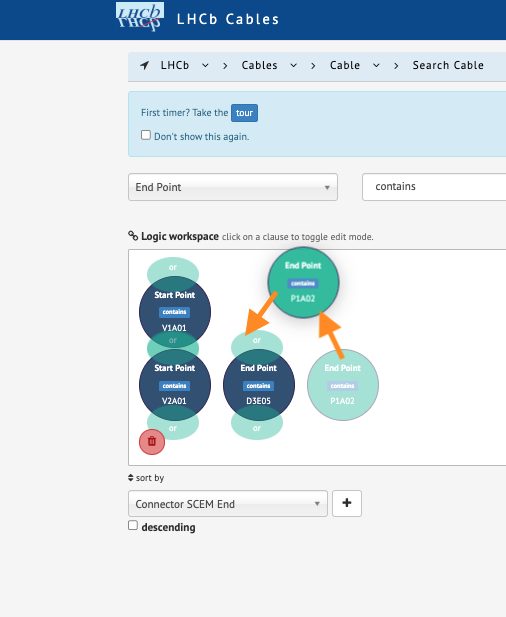
\includegraphics[width=\linewidth]{figuras/fence_search_1_sm.png}
        \caption{Query workspace.}
        \label{fence-ss-1}
    \end{minipage}
    \hfill
    \begin{minipage}[t]{.4\textwidth}
        \centering
        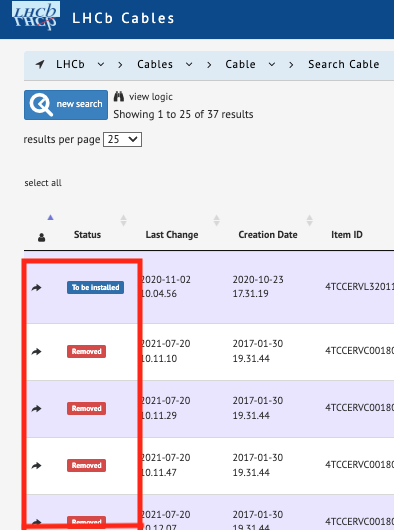
\includegraphics[width=\linewidth]{figuras/fence_search_2_sm.png}
        \caption{Fence search results.}
        \label{fence-ss-2}
    \end{minipage}
\end{figure}

\paragraph{} To provide a replacement for the SuperSearch, the main inspiration was Jira's Query Language \cite{jirajql}. Jira is a software tool developed by Atlassian that allows bug tracking, issue tracking, and agile project management. Jira Software supports different agile project management methodologies for software development, providing tools to estimate, report, and measure velocity with workflows designed to fit your frameworks. Since many years, it has been the officially supported issue tracker software at CERN. \cite{jirajql}

\paragraph{} As described by Dan Radigan \cite{jirajql}, Jira Query Language (JQL) is a flexible tool developed by Atlassian for searching issues in Jira. The key features of JQL (Jira Query Language) include advanced search capabilities, allowing users to perform complex searches using a structured query language; customizable queries, where users can create queries based on specific fields, operators, and values; and a syntax similar to SQL, making it intuitive for those with database query experience. The components of JQL consist of fields, which are the data points in Jira such as priority, status, and assignee; operators, which define the relationship between fields and values, with examples including ``=", ``!=", ``$\ge$", and ``$\le$"; and values, which are the actual data or criteria being queried. 

\paragraph{} Souza e Silva \cite{SouzaSilva2023Glance} describes similar definitions for the structured query language used on the new Super Search which was called Glance Search Library. On \cite{SouzaSilva2023Glance}, the Glance Query Language (GQL) is described as a pivotal aspect of the new architecture, being used on the server-side to convert query strings into SQL filters, forming a $WHERE$ clause by mapping query string elements (Eg.: table names, table columns, boolean operators) into SQL elements through a JSON configuration file. This design differs from FENCE's Super Search by limiting the JSON file's scope to mapping query string elements to database columns and caching settings, thus making the frontend interfaces independent of this file. 

\paragraph{} Using the same example from \cite{SouzaSilva2023Glance} to find \textit{all cables that start in point A and end in point C plus all cables that start in point B and end in point D} this would be written in GQL as 

\begin{multline*}
queryString_1: \text{(start\_point = PointA \textbf{AND} end\_point = PointC)} \\
\text{\textbf{OR} (start\_point = PointB \textbf{AND} end\_point = PointD)}
\end{multline*}

\noindent
And the GQL equivalent of the query that could be composed through FENCE's SuperSearch is \begin{multline*}
queryString_2: \text{(start\_point = PointA \textbf{OR} start\_point = PointB)} \\
\text{\textbf{AND} (end\_point = PointC \textbf{OR} end\_point = PointD)}
\end{multline*}

\noindent
With the GQL elements categorized in the table \ref{table:search-elements}.

\begin{longtable}{|p{0.25\textwidth}|p{0.5\textwidth}|p{0.25\textwidth}|}
\caption{Search elements}\label{table:search-elements} \\
\hline
\textbf{Element} & \textbf{Category} & \textbf{Identifier} \\ \hline
\endfirsthead

\multicolumn{3}{c}%
{{\bfseries \tablename\ \thetable{} -- continued from previous page}} \\
\hline
\textbf{Element} & \textbf{Category} & \textbf{Identifier} \\
\hline
\endhead

\hline
\endfoot

Start point & \textbf{Search Field} & $f_1$ \\
End point & \textbf{Search Field} & $f_2$ \\
= & \textbf{Search Operator} & $o_1$ \\
AND & \textbf{Search Conjunction} & AND \\
OR & \textbf{Search Conjunction} & OR \\
Point A, B, C, D & \textbf{Search Value} & $v_1, v_2, v_3, v_4$ \\
( & \textbf{Grouping Mark} & ( \\
) & \textbf{Grouping Mark} & ) \\
\hline
\end{longtable}


A \textbf{Search Statement} in GQL is a combination of a Search Field, Operator, and Value. For instance, from the queries, four statements are derived: $s_1: f_1 \frown o_1 \frown v_1$, $s_2: f_2 \frown o_1 \frown v_3$, $s_3: f_1 \frown o_1 \frown v_2$, and $s_4: f_2 \frown o_1 \frown v_4$ where ``X" $\frown$ ``Y" $\frown$ ``Z" denotates the concatenation of the SearchField ``X", a space character, the SearchOperator ``Y", another space chacters plus the SearchValue ``Z". Rewriting the query strings as a funcion of the statements $queryString_1$: ($s_1$ $\land$ $s_2$) $\lor$ ($s_3$ $\land$ $s_4$) and $queryString_2$: ($s_1$ $\lor$ $s_3$) $\land$ ($s_2$ $\lor$ $s_4$). The design of GQL, decoupled from interface and infrastructure constraints, ensures that both queries are valid, resolving the limitations encountered in the FENCE system where $queryString_1$ could not be created.

\paragraph{} With GQL, it is already possible for users to perform a search by typing the query string in a text input. However, in order to assist users with the query formulation and prevent syntax errors, an interface component to handle advanced boolean searches had to be built. Because users were very familiar with FENCE's SuperSearch as it was in use for many years, the new solution should resemble the query composition mechanism to reduce the learning curve. This means going against most UX research, which tends to favor simpler search interfaces, as discussed on \cite{Nielsen2001SearchVisible}. In this article, titled ``Search: Visible and Simple", the author gives some general guidelines on how to handle search in a web application. The author emphasizes the importance of maintaining a straightforward and accessible search interface in web applications. This approach is grounded in the observation that users generally prefer and perform better with simpler search mechanisms. Complex or advanced search interfaces, while potentially powerful, can often lead to user confusion and frustration, especially for those not skilled in intricate query formulation. The article suggests that a basic search box is usually sufficient for most users’ needs, and its prominent placement, preferably on the homepage, enhances usability. Moreover, the design should focus on optimizing first-time search success, as users' likelihood of finding desired results diminishes with each subsequent search attempt. The author argues that, while advanced search capabilities may have their place, especially in specialized applications, they should not overshadow the simplicity and accessibility of the primary search function. This perspective challenges the idea of replicating the complex mechanisms of FENCE's SuperSearch, proposing instead that a more user-friendly approach, with an emphasis on simplicity and visibility, could lead to a more effective and efficient search experience for the majority of users.

\paragraph{} At the same time, other publications, such as ``How to Design Advanced Search Interface – Step by Step" by Abhijit Rawool \cite{RawoolAdvancedSearch}, acknowledge the necessity of an advanced boolean search interface and give general guidelines for improved usability. Rawool argues that while advanced search might not be essential for all applications, it plays a crucial role in complex systems like enterprise-level applications. He suggests a thoughtful approach to implementing advanced search, emphasizing that it should only be used when simple search fields are insufficient. Rawool recommends starting with a quick search interface and then providing an option for advanced search, echoing the sentiment that basic search meets most users' needs. However, when more detailed searches are required, advanced search interfaces become valuable. He advises careful consideration of the user interface (UI), suggesting that the advanced search form should be hidden initially and only made visible when the user opts for more detailed search criteria. In designing advanced search forms, Rawool highlights the importance of user effort in interpreting these interfaces. Each field in the advanced search should be clearly labeled and intuitive to use, minimizing the cognitive load on users. Furthermore, he advocates for including clear or reset buttons, allowing users to easily start their search over, which is particularly helpful given the larger number of fields in advanced search forms. Additionally, Rawool addresses the potential clutter of numerous search fields. He proposes the ``Add Fields" feature, where users can customize their search by adding additional fields as needed, keeping the interface clean and user-focused. This approach not only declutters the interface but also empowers users to tailor their search experience according to their specific needs.

\paragraph{} These publications played a crucial role in the decision to build a modular search interface based on web components. A web component is essentially a self-contained, reusable module in a web application. It encapsulates HTML, CSS, and JavaScript, allowing developers to create custom, encapsulated HTML tags for use in web pages and apps. This design choice gives developers the flexibility to customize the interface, allowing them to add necessary features and remove those that are not needed for a particular use case. Another important decision was to combine the query composition area with the search results display. This was based on the observation that users often perform searches without applying any filters, just to see a full list of entities (eg.: loading the information of all institutes). By merging these two interfaces, the system can cache this list, giving a snappier feel to the user. The final decision involved adding a quick lookup search (also known as simple search) on the homepage and fixed in the navigation bar. This was influenced by the recommendations from \cite{Nielsen2001SearchVisible} and \cite{RawoolAdvancedSearch}, which emphasize the importance of having an always visible search feature. This is particularly useful for instances where a user wants to search for a specific entity, such as a member searching for their institution. In such cases, the simple search will accept a string as input and return the link for the entity's profile in the system.


\paragraph{} In order to build a component based web interface it is necessary to map the fundamental components and how they will interact with each other.  An Event Storming workshop was used to map such components as described by Michelly Teixeira on \cite{michelly} . This workshop was a collaborative effort to clarify the business logic behind the search functionality and model its components effectively.


\paragraph{} Event Storming helped the team map the search process using sticky notes on a virtual board, leading to the identification of domain events, user actions that triggered these events, and their organization into a timeline. The session began with brainstorming to define relevant events for the user and system, which were then associated with user or system actions that triggered them. The exercise provided insights into the actions, entities, and actors involved in the search process. Subsequent meetings analyzed these insights to define the search interface components, detailing the properties each component should access and manage, resulting in two main views: the Filters View and the Results View. A state management pattern library was chosen to manage communication between components, centralizing the state to handle the search interface more effectively. The final result documented each component's role in generating commands and consuming events. Interface mockups were created to visualize the web components, exploring the possibility of merging search inputs and results into a single view for a more responsive user experience.


\section{The LHCb Membership}
\paragraph{} As already discussed in the introduction, the LHCb is a geo-distributed scientific collaboration that specializes in investigating the slight differences between matter and antimatter by studying a type of particle called the ``beauty quark" \cite{LHCb_Description}. The LHCb Membership is a system used to manage the collaboration participants, automatizing bureaucratic processes and enforcing the rules defined in the LHCb Constitution \cite{LHCbConstitution}. The main users of the LHCb Membership System are the LHCb Management, the Editorial Board (EB), the Membership Committee, the Secretariat and Institute and Country Representatives. As of February 2024 LHCb has 97 universities and research centers associated from 23 countries and 1656 members.

\subsection{Collaboration organization}

\paragraph{} The LHCb Constitution \cite{LHCbConstitution} defines a series of roles in the collaboration. The most relevant roles for the Membership context are described below.

\paragraph{} The LHCb Management serves as the executive body responsible for the operation of the detector, its upgrades, and physics analysis. It represents the LHCb Collaboration to external entities and comprises the Spokesperson, Deputy Spokespersons, Technical Coordinator, and Resources Coordinator. Advised by the Technical Board, Operations Planning Group, and Physics Planning Group, the LHCb Management makes daily decisions and communicates relevant issues to the Collaboration Board (CB).

\paragraph{}Major decisions by the Management are reported to the Plenary Meeting and then to the CB for endorsement. In urgent situations, where decisions cannot wait for a CB meeting, the Chairperson of the CB is consulted, and the decision is reviewed at the subsequent CB meeting. The Management maintains open communication with CERN Management and organizes resources, preparing the LHCb budget for presentation to the CB and the Resources Review Board. Additionally, the Management nominates Project Leaders and the Operations Coordinator, subject to CB approval, and may establish ad hoc Working Groups, recommending Conveners to the CB.

\paragraph{}The Spokesperson, as head of the LHCb Management, officially represents the collaboration and is the primary contact between LHCb, CERN Management, and the LHCC. Elected by the CB, the Spokesperson holds ultimate responsibility for the experiment and has authority over the production and dissemination of physics results, reporting directly to the CB.

\paragraph{}Deputy Spokespersons, nominated by the Spokesperson and ratified by the CB, represent the Spokesperson in their absence and may take on specific responsibilities, with any significant delegations being reported to the CB. They are non-voting, ex officio members of the CB, Operations Planning Group, Technical Board, and Physics Planning Group, and their term ends with the Spokesperson's term.

\paragraph{}The Resources Coordinator, nominated by the Technical Coordinator with the Spokesperson's agreement and ratified by the CB, oversees financial planning. This includes establishing annual budgets and expenditure reports for the CB and LHCb Resources Review Board, monitoring payments, and managing the implementation procedure for late M\&O (maintenance and operation) fund contributions. The Resources Coordinator reports to the Technical Coordinator and the CB and is an ex officio member of both the Technical Board and the CB. These are heavy users of the Membership, as the M\&O fee paid by the universities and research centers is a function of their number of members. 

\paragraph{}The LHCb Editorial Board (EB) oversees the collaboration's publication standards, with members appointed by the Spokesperson and ratified by the Collaboration Board. Terms are two years, with staggered renewals for continuity. The EB manages the review process for publications, ensuring the collaboration's input is incorporated and the proper authors list is used. In case of disputes, decisions are made by the EB Chairperson, Physics Coordinator, and Spokesperson. The EB also maintains a database of official LHCb results and materials.

\paragraph{}The LHCb Authorship rules in \cite{LHCbConstitution} state that collaborators earn the right to sign physics papers by contributing to the experiment, including detector construction, real-time analysis, online projects, computing projects, data taking, calibration, or data processing. Institutes must engage in service tasks as well. Authorship begins six months after joining LHCb and extends for 12 months post-membership. Annually, institutes submit a default author list, influenced by their M\&O budget share. PhD students are not bound by this quota. Retired active members can gain Emeritus status, allowing them to sign papers without M\&O and service obligations, subject to annual confirmation and support from LHCb coordinators or the Spokesperson. Authors can opt out of signing a paper, and exceptions to these rules are handled by the Editorial Board Chairperson, the Spokesperson, and the relevant institute leader, with a possible appeal to the Spokesperson. The Editorial Board reports to the CB on exception requests. The list is created and managed by the Authorship system which is a part of the Membership.

\paragraph{}LHCb membership comprises two types: Institute and Individual. Institute membership concerns CB treatment, while Individual membership involves status and access rights. The Membership Committee, set up by the CB and Management, reviews applications and participation in essential tasks. The Committee is formed after each CB chair election and reports to the CB.

\paragraph{} New institutes express interest to join LHCb through a letter, followed by a meeting with the Spokesperson and CB Chairperson to draft a detailed application, including contributions and service task plans. The Membership Committee reviews the application, and the institute presents its contributions to the CB. Admission requires two-thirds CB vote support. If positive, the institute is included in the M\&O sharing and recognized by the LHC Resource Review Board. Institutes may also become Associated or Technical Associated Members.\paragraph{} Individual membership for members from existing LHCb institutes is managed by their institute leader, who also notifies the LHCb secretariat of departures.  Significant growth in an institute's size is communicated to the CB Chair and Spokesperson, detailing resource and contribution changes for evaluation by the Membership Committee and CB.

\paragraph{} Associated Membership is for institutes contributing to specific projects, hosted by an LHCb institute, and responsible for long-term maintenance. They don't have a CB vote but are represented by their host and are eligible for LHCb authorship.  Technical Associated Membership is for institutes contributing to detector or computing projects, without access to data or LHCb authorship, but they may participate in hardware and software development.

\paragraph{} Individual membership categories vary by status and access rights, with different levels of affiliation and authorship conditions. Full members have full access and primary affiliation, while Technical and Software Associates have restricted access tied to specific projects. Affiliates, such as theorists, have short-term full access, with potential authorship on individual papers. Access rights and full membership are subject to approval and cannot be granted to individuals from Technical Associated Member institutes. M\&O contributions are expected from full member academics and postdocs.

\paragraph{} The LHCb Secretariat plays a key role in the collaboration management. Once a member or institution is accepted in the collaboration, they operationalize their registration procedures.  They also monitor the affiliation statuses and provide support with CERN's bureaucratic processes.

\paragraph{} Therefore, the major roles for the Membership context are summarized in table \ref{table:LHCbRoles}.


\begin{longtable}{|p{0.4\textwidth}|p{0.55\textwidth}|}
\caption{Major roles in LHCb for the Membership}\label{table:LHCbRoles} \\
\hline
\textbf{Role} & \textbf{Responsibilities and Characteristics} \\ \hline
\endfirsthead

\multicolumn{2}{c}%
{{\bfseries \tablename\ \thetable{} -- continued from previous page}} \\
\hline
\textbf{Role} & \textbf{Responsibilities and Characteristics} \\
\hline
\endhead

% Now, list each role with its responsibilities
Spokesperson and Deputy & Represents the collaboration, primary contact between LHCb and CERN Management, ultimate responsibility for the experiment. Elected by the CB. \\
\hline
Technical Coordinator & Part of the LHCb Management, advises on technical aspects of the detector and its upgrades. \\
\hline
Resources Coordinator & Oversees financial planning, monitors payments, and manages the M\&O fund contributions. Reports to the Technical Coordinator and the CB. \\
\hline
Project Leaders & Nominated by the Management, subject to CB approval, lead specific projects within the collaboration. \\
\hline
Editorial Board (EB) & Oversees publication standards, manages review process for publications, and maintains a database of official LHCb results. Members appointed by the Spokesperson and ratified by the CB. \\
\hline
Membership Committee & Reviews applications for Institute and Individual membership, reports to the CB. Formed after each CB chair election. \\
\hline
Institute Members & Involved in CB treatment, participate in M\&O sharing, can be Full, Associated, or Technical Associated Members. \\
\hline
Individual Members & Vary by status and access rights, managed by institute leader, include Full members, Technical and Software Associates, and Affiliates. \\
\hline
LHCb Secretariat & Manages registration procedures, monitors affiliation statuses, provides support with CERN’s bureaucratic processes. \\
\hline
Administrators & Glance developers and project managers \\
\hline
\end{longtable}




\subsection{Business requirements}
\paragraph{} The LHCb Membership System is used to manage the affiliations of \textbf{Member}s and \textbf{Institute}s (universities and research centers) with LHCb. Institutes, upon joining LHCb, open a \textbf{Participation} (which can be official, associated, technical, only for authorship and other types) with a period.  The Membership integrates with CERN's Human Resource (HR) systems and provides information to other applications that need to consume the list of Members. Members are affiliated with Institutes through one or multiple \textbf{Employment}s. The Employment includes information such as the affiliation type (primary or secondary), the \textbf{Profession}, flags to determine whether a member is entitled to authorship and counts for M\&O and the affiliation period. Members can also be assigned to special roles (Spokesperson, Team Leader, Safety Officer and more) which are called \textbf{Appointment}s. An Appointment may have an associated \textbf{Country} (eg.: for Country Representative), Institute (eg.: for Team Leader) or \textbf{Physics Working Group}. For the Authorship, there can be \textbf{Exception}s which are Members added to a specific \textbf{Paper}'s list of authors due to their exceptional contributions or members who requested to be removed from the paper. It is also possible to add \textbf{External Author}s affiliated with LHCb Institutes or \textbf{External Institute}s. \textbf{Funding Institution}s can also be acknowledged on a paper basis due to financial \textbf{Grant}s provided to Members or Institutes.

\paragraph{} The LHCb Membership Version 1 was essentially a CRUD system, providing digital forms for users to fill in the registration details for the entities just listed and search interfaces to retrieve these instances' information. It also sent periodic notifications using job schedulers. During the rewrite, all the CRUD functionality had to be implemented in the new stack, but the team used the opportunity to better understand how the processes in the collaboration worked in real life  and tailor the system to better fit the user needs. The table \ref{table:lhcb_membership_requirements}, lists the Membership System requirements. The requirements marked with an asterisk (*) will be enriched in the Workflow Project, aimed at transitioning real-life approval workflows into the Membership system. This transition involves multiple roles collaboratively reviewing and signing off on a document, ultimately leading to a specific outcome or action being recorded in the Membership database. Requirements marked with ``**" could only be implemented in the new stack, as FENCE's rigid architecture made them unfeasible.


\begin{longtable}{|p{0.05\textwidth}|p{0.45\textwidth}|p{0.4\textwidth}|}
\caption{LHCb Membership System Requirements and Role Access} \label{table:lhcb_membership_requirements}\\
\hline
\textbf{\#} & \textbf{Requirement Title \& Description} & \textbf{Roles Access} \\
\hline
\endfirsthead

\multicolumn{3}{c}%
{{\bfseries \tablename\ \thetable{} -- continued from previous page}} \\
\hline
\textbf{No.} & \textbf{Requirement Title \& Description} & \textbf{Roles Access} \\
\hline
\endhead


\hline
\endlastfoot

1 & Display User Info: Users can view other Member's information. & Basic User, Administrator, Secretariat \\
\hline
2* & User Registration: Administrators can insert new Members with specific rules. & Administrator \\
\hline
3 & Member Edition: Allows editing of Member details. & Administrator \\
\hline
4 & User History Tab: Users can view their profile updates. & Basic User, Administrator, Secretariat \\
\hline
5 & Search User: Users can search for other Members. & Basic User, Administrator, Secretariat \\
\hline
6 & Institute Insertion: Administrators can add new Institutes with specific rules. & Administrator, Secretariat \\
\hline
7 & Institute Edition: Allows updating Institutes' basic info. & Administrator, Secretariat \\
\hline
8 & Institute Details: Viewing of Institutes' basic and Employment info. & Basic User, Administrator, Secretariat, Team Leader \\
\hline
9 & Institute History Tab: Users can see updates to Institutes. & Basic User, Administrator, Secretariat \\
\hline
10 & Search Institute: Enables searching for Institutes. & Basic User, Administrator, Secretariat \\
\hline
11 & Employment End Notification: Notifies specific roles before Employment ends. & Administrator, Secretariat \\
\hline
12* & Add Employment: Administrators and Secretariat can add Employment for users with rules. & Administrator, Secretariat \\
\hline
13* & Update Employment: Administrators and Secretariat update Member's Employments. & Administrator, Secretariat \\
\hline
14 & Employments Tab: Viewing of user's Employment records. & Basic User, Administrator, Secretariat, Team Manager \\
\hline
15** & Display Statistics for Institutes: Visualize Institute statistics. & Basic User, Administrator, Secretariat \\
\hline
16** & Display Statistics for Countries: Country Representatives can view Country statistics. & Administrator, Secretariat, Country Representative \\
\hline
17 & Public Page for Authors List: Access to LHCb authorship list for a given date for unlogged users. & Public \\
\hline
18 & Upcoming Employment Notification: Advance notification about upcoming Employments. & Administrator, Secretariat \\
\hline
19 & Institute Change Notification: Notifies Team Leaders about Institute Participation changes. & Administrator, Secretariat, Team Manager \\
\hline
20 & Notification of Legacy Members: Semi-annual check for possible duplicates of old Members. & Administrator, Secretariat \\
\hline
21 & Summary M\&O Report: Access to summary reports for specific roles. & Administrator, Secretariat, Resource Coordinator, Team Manager \\
\hline
22 & Detailed M\&O Report: Detailed M\&O reports with access for specific roles. & Administrator, Secretariat, Resource Coordinator, Team Manager \\
\hline
23 & Add Warning to Update Appointment End Date: Synchronization or warning for appointment end dates. & Administrator, Secretariat \\
\hline

\end{longtable}

\paragraph{} Differently from the Membership System that already had a working version and a set of requirements reasonably fulfilled, the Authorship system requirements were not clear and the only document available was the LHCb constitution \cite{LHCbConstitution} that lacks in details and do not cover corner cases. To gather the Authorship system requirements, the developers organized a series of customer interviews, which, based on \cite{CustomerInterview}, are a qualitative research method aimed at understanding users' needs, preferences, experiences, and challenges with a software product. This process involves planning the interview objectives, recruiting representative participants, conducting interviews with open-ended questions, analyzing the responses to identify common themes, and using the insights to guide development decisions. The practice ensures a user-centric design, as it provides direct feedback from users or potential users, helping to validate assumptions, identify pain points, and inform feature prioritization. 

\paragraph{} This effort resulted in an internal document describing the rules for a Member to be considered an Author:
\begin{itemize}
    \item The Member should have the ``full member'' membership access status;
    \item The current Employment Profession is neither Master Student nor Bachelor Student;
    \item The Member has an active Employment entitled to authorship OR the last Employment entitled to authorship ended in one year at most before the reference date;
    \begin{itemize}
        \item The second condition is taken into account for Members that fully terminated their LHCb membership and also for Members that switched from an affiliation entitled to authorship to an affiliation not entitled to authorship. This way, the system ensures fairness by applying the 1 year grace period to both active and inactive Members;
    \end{itemize}
    \item The sum of the periods of Employments entitled to authorship is $\geq 6$ months (180 days);
    \begin{itemize}
        \item Every Employment entitled to authorship started before the reference date is counted (even the ones ended more than 1 year ago);
        \item Overlapping primary and secondary Employments are not counted twice;
        \item By default, an Employment is entitled to authorship when the profession is one of the following: Emeritus, PhD Engineer, Post Doc, PhD Student, or Senior.
    \end{itemize}
\end{itemize}

\noindent
 Alongside the more precise authorship rules, the system requirements were gathered and are listed in the table below. An \textbf{Authorship} list can be compiled for a given date of for a given paper. Exceptions are only added to papers' authors lists. 

\begin{longtable}{|p{0.05\linewidth}|p{0.25\linewidth}|p{0.65\linewidth}|}
\caption{Authorship System requirements} \\
\hline
\textbf{\#} & \textbf{Title} & \textbf{User Story \& Notes} \\
\hline
\endfirsthead

\multicolumn{3}{c}%
{{\bfseries Table \thetable\ continued from previous page}} \\
\hline
\textbf{\#} & \textbf{Title} & \textbf{User Story \& Notes} \\
\hline
\endhead

\hline
\endfoot

\hline
\endlastfoot

1 & Display Paper Interface & A user wants to visualize all papers and their information in a table. This includes paper status, identifier, title (supporting latex), number of authors, exceptions, reference date, and admin functions (export, delete, edit). \\
\hline
2 & Search Paper & A user wants to search already created paper by paper title. \\
\hline
3 & Download Paper & A user wants to export the authorship list in various formats: arXiv latex, InSpire xml, simple latex, PDF, and lists grouped by institute. \\
\hline
4 & Remove Paper & An admin wants to remove a non-published paper. \\
\hline
5 & Manage Paper & An admin wants to manage an ``on going" paper, with capabilities to remove/add authors, change paper status to published, and add institutes. \\
\hline
6 & Exceptions Summary & An admin wants to visualize a summary of the authors and institutes added or removed from the authorship list. \\
\hline
7 & External Authors & An admin can add authors from outside the LHCb collaboration, requiring details like initials, author name (in English), latex name, Inspire, ORCiD, and institute affiliations. \\
\hline
8 & External Institutes & If the author is from an external institute, it can be added with details like institute name, city, country, and main affiliation status. \\
\hline
9 & Create Paper & An admin can create a new paper, specifying details like paper title (supporting latex), reference date, a unique custom paper identifier, and an optional CDS link. The default paper identifier format is detailed. \\
\hline
10 & Preview Authorship List & A user wants to preview the list ordered by last name, with the ability to filter by institute and clearly see all external members/institutes added or removed. \\
\hline
11 & Authorship for a given date & A user wants to preview the authorship list for a given date \\
\hline
12 & Download Authorship for date & A user wants to download the authorship list for a given date \\
\hline
13 & Register Funding Agency & An admin or Secretariat wants register a Funding Agency \\
\hline
14 & Register/Manage Grant & An admin or Secretariat wants to register/update/delete a financial Grant provided by a Funding Agency to a Member or Institute \\
\hline
15 & Register/Manage Grant & An admin or Secretariat wants to register/update/delete a financial Grant provided by a Funding Agency to a Member or Institute \\
\hline
16 & Acknowledge Grant & The EB Chair wants to acknowledge a Grant in a Paper's authors list \\

\end{longtable}

\paragraph{} With the requirements gathering process concluded, the author started to develop mock interfaces, which were again validated with the EB. This marks the start of the migration to a new software architecture in the LHCb Glance systems.

\paragraph{} The Authorship was very modified a second time at the beginning of 2023 due to the Russia-Ukraine conflict which, in February 2022, escalated significantly when Russia launched a full-scale invasion of Ukraine, marking a substantial increase in hostilities and leading to widespread international condemnation, additional sanctions against Russia, and a humanitarian crisis. The conflict has had far-reaching implications, including economic disruptions, an energy crisis in Europe, and concerns about broader regional or global security implications. In response to the complex dynamics and personal convictions stemming from the conflict, the EB decided to first allow authors to hide their affiliations on the authorship lists. This decision was made to accommodate authors who wished to dissociate themselves from their institutions, particularly those affiliated with Russian institutes, due to disagreements with their institution's stance or the broader political situation. Subsequently, the EB also permitted authors to completely remove their names from authors lists including Russian institutes if they chose to, reflecting a stance of personal or ethical disagreement. This necessitated modifications to the authorship algorithm to support these requests, ensuring that authors could exercise their choices regarding affiliation visibility and participation in a manner consistent with their principles and the evolving situation. The final directive issued by the Editorial Board (EB) implied in the exclusion of all Russian institutes from the author lists, reinforcing LHCb's stance of condemning the actions undertaken by Russia. 



\subsection{Workflow Project}
\label{subsec:workflow_project_cap_2}
\paragraph{} While exploring the possible architectural patterns for the new refactor projects, the developers came across the Ubiquitous Language and Domain Driven Design (DDD) concepts.  Eric Evans, in his book ``Domain-Driven Design"  \cite{evans2003domain}, defines a software development approach centered around modeling software to faithfully reflect the core concepts and rules of a specific domain. This philosophy, deeply rooted in understanding the domain itself, emphasizes building software that aligns with business needs and adapts to complexity. The fundamental pillar of Evans' DDD rests on ubiquitous language, a shared vocabulary established by developers and domain experts. This common language ensures everyone operates on the same page, reducing communication gaps and fostering collaboration. It's through this language that the domain model emerges, a conceptual representation of the core entities, their relationships, and the domain's inherent rules.  

% Maybe I'll need something to support this user pain thing
\paragraph{} A significant challenge identified with Membership V1 was its constrained functionality within collaboration procedures, particularly evident in the newcomer registration process. This limitation is illustrated in the flowchart referenced in Figure \ref{fig:registration_old}. The flowchart delineates tasks executed by newcomers in yellow and those undertaken by the LHCb Secretariat in orange. A holistic analysis reveals the LHCb Membership's restricted application and its susceptibility to errors, primarily due to the Secretariat's potential need to manually input information from numerous PDF forms into the system. Also, the redundancy of data entry is another critical issue; information solicited through the LHCb registration form PDF, shown in Figure \ref{fig:lhcb_registration_form_pdf}, often duplicates data already present in CERN's HR system. This duplication not only burdens users with repetitive data entry tasks but also heightens the risk of data inconsistencies across different platforms.

\begin{figure}[H]
    \centering
    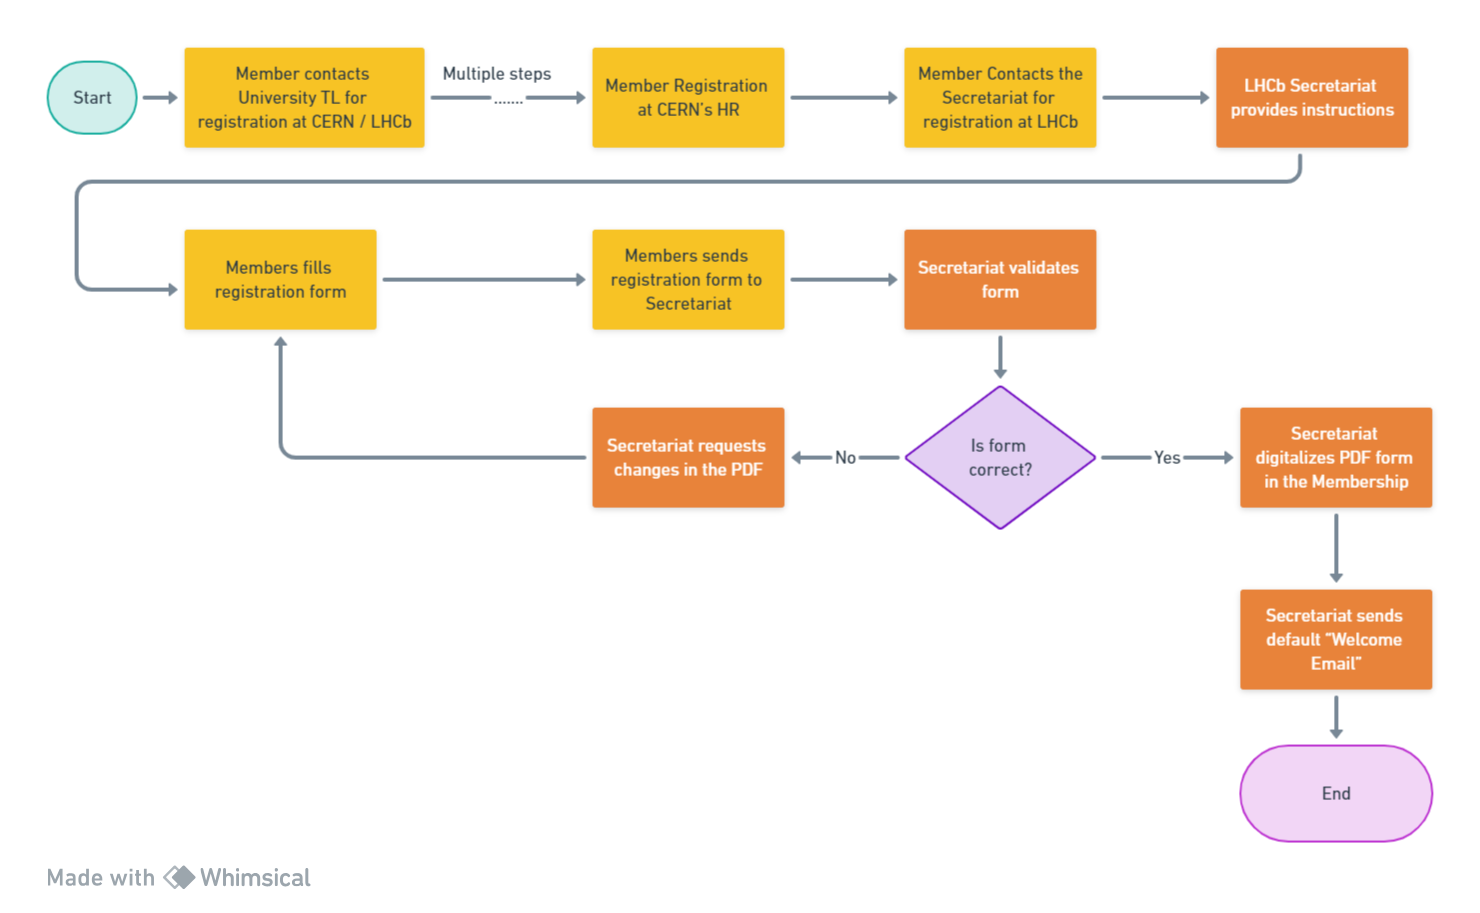
\includegraphics[width=1\linewidth]{figuras/newcomer_wf.png}
    \caption{LHCb newcomer registration procedure.}
    \label{fig:registration_old}
\end{figure}

\begin{figure}[H]
    \centering
    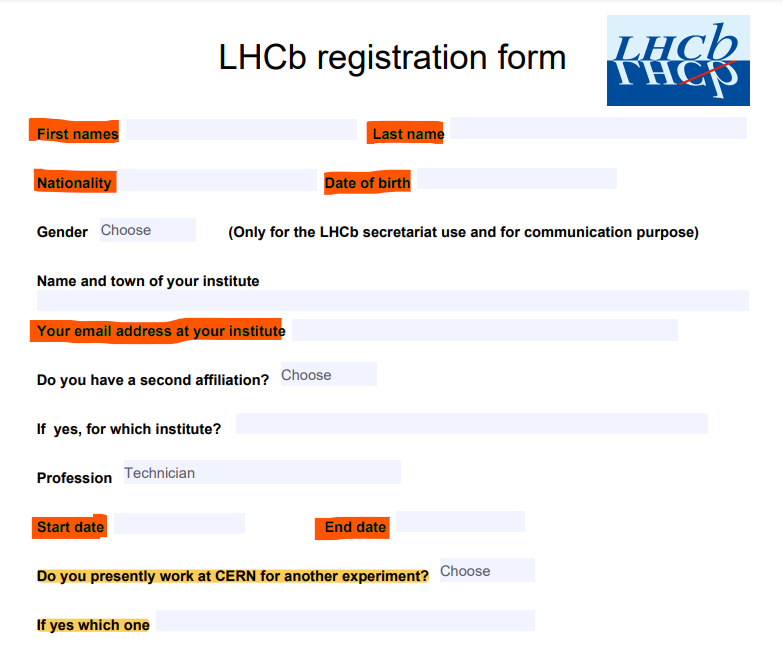
\includegraphics[width=0.6\linewidth]{figuras/lhcb_form.png}
    \caption{LHCb newcomer registration PDF form. All information highlighted in red is already present in CERN's HR database once this form is filled by the newcomer.}
    \label{fig:lhcb_registration_form_pdf}
\end{figure}

\paragraph{} In contrast to traditional CRUD systems like Membership V1, which primarily focus on the basic operations of data persistence and manipulation DDD emphasizes the modeling of the domain's intricacies and its fundamental principles, facilitating the creation of software that is highly congruent with business objectives and capable of evolving alongside them. Specifically, in the context of the workflow depicted in Figure \ref{fig:registration_old}, DDD advocates for more atomic actions. An example would be implementing a feature that allows the Secretariat to directly reject a registration form with a single click, which would then automatically trigger an email notification to the newcomer, prompting them to amend their submission. Additionally, a scheduled task could regularly check CERN's HR systems for new registrations, automatically initiating the LHCb registration process by firing email notifications with the necessary instructions through a static page on the Membership platform. These enhancements, derived from discussions with key users of the Membership system, aim to streamline and enrich the user experience. Further, additional workflows have been identified and mapped to extend the system's functionality, including the modification of Employment profession, the extension of Employment periods, and the creation of new Employment records. 

\paragraph{}These enhancements highlight the transformative capacity of Domain-Driven Design (DDD) in redefining system architecture, ensuring it mirrors the details of real-world business operations and addresses the needs of its users effectively. Furthermore, this approach has motivated the creation of software tools capable of monitoring the lifecycle of entities through approval workflows. The conceptual diagram, referenced in Figure \ref{fig:cap_2_workflow_draft}, provides a view of the proposed workflow tracking mechanism. This model documents all conceivable \textbf{States} (represented by circles) an entity might occupy, alongside \textbf{Transitions} (depicted by arrows) between these States. A Transition is initiated once all requisite \textbf{Conditions} are met. The envisioned Workflow Tracker would monitor \textbf{Events}, marking a Condition as fulfilled upon the occurrence of a corresponding Event. This system is designed to inform an Entity of its current State, potential subsequent States, and the Conditions necessary for progression.

\begin{figure}[H]
    \centering
    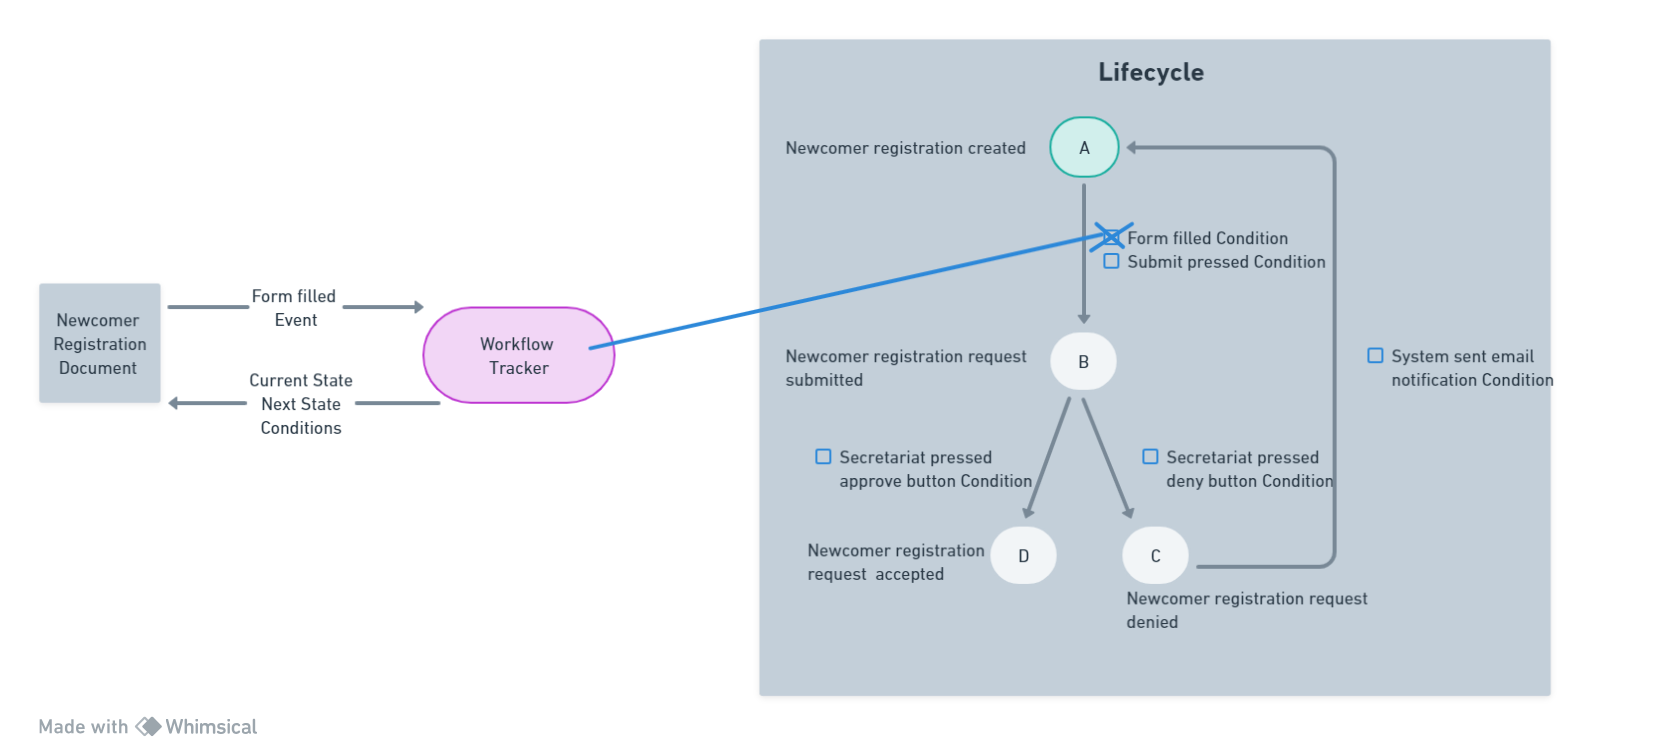
\includegraphics[width=1\linewidth]{figuras/workflow_draft.png}
    \caption{Workflow Tracking Service draft.}
    \label{fig:cap_2_workflow_draft}
\end{figure}

\paragraph{} A more formal version of the draft displayed in Figure \ref{fig:cap_2_workflow_draft} becomes a necessity for the LHCb Analysis Lifecycle Management System (ALCM) \cite{alcm}. This system manages the lifecycle of graphs, such as plots and diagrams, papers, conference notes, and other documents published by the Collaboration. The documents undergo an approval process, involving validation by various Collaboration members based on their appointments. For instance, during parts of the process, the Physics Coordination must approve the document, affirming the content's accuracy. Subsequently, the Editorial Board provides a sign-off, focusing on grammar and formatting. The initial idea was for the ALCM to reuse the same classes created for the Membership Workflow Tracker, but during the planning phase of the project, the developers realized that a more robust solution based on the graph theory would be needed.


\subsection{Discrete-Event Systems}

\paragraph{} A Discrete Event System (DES) can be conceptualized as a mechanism governed by state changes triggered by discrete events. These systems are characterized by a discrete state space and are event-driven. An event refers to any instantaneous occurrence that can lead to a transition in the state of the system. Formally, the set of possible events in a network can be denoted as:
$$
\Sigma=\{p, q\}
$$
where \(p\) represents the arrival of a packet, and \(q\) signifies that the packet queue is full. This scenario encapsulates the dynamism and responsiveness of DES in managing network traffic, where each event (such as the arrival of a new packet or reaching the capacity of a packet queue) precipitates a change in the operational state of the network.

\paragraph{} For a given set \(\Sigma\), its Kleene closure, \(\Sigma^*\), represents the totality of all possible finite-length sequences that can be constructed from the elements of \(\Sigma\), including the empty sequence denoted by \(\epsilon\).

\paragraph{} Example:

\[
\begin{gathered}
\Sigma = \{x, y, z\} \\
\Sigma^* = \{\epsilon, x, y, z, xx, xy, xz, yx, yy, yz, zx, zy, zz, xxx, \ldots\}
\end{gathered}
\]

\paragraph{} This comprehensive collection \(\Sigma^*\) encompasses every conceivable language \(L\) that can be derived from \(\Sigma\), ensuring that \(L\) is either fully contained within or exactly equals \(\Sigma^*\). This includes the specific sets \(\Sigma^*\), \(\Sigma\), and \(\emptyset\). Notably, the empty set \(\emptyset\) is distinct from \(\{\epsilon\}\), which contains a single element, namely the empty sequence \(\epsilon\).

\paragraph{} Consider a sequence \(s = \text{def}\). The segments ``d", ``e", and ``f" of \(s\) correspond to its prefix, subsequence, and suffix, respectively. Therefore, the sequence can be viewed in several relational contexts:
\[
s = s \epsilon, \quad s = \epsilon s, \quad s = \epsilon s \epsilon
\]
In these relations, \(\epsilon\) serves as a universal prefix, suffix, and subsequence for any string, including \(s\).

\noindent 
Example:
\[
s = \text{xyz}
\]
Prefixes of \(s = \{\epsilon, x, xy, xyz\}\). Suffixes of \(s = \{\epsilon, z, yz, xyz\}\).

\paragraph{} In formal language theory, standard set operations such as union, intersection, difference, and complement are applicable to languages since they are sets. For subsets \(L_a\) and \(L_b\) within \(\Sigma^*\), their concatenation is defined as:
\[
L = L_a L_b = \{s = s_a s_b \in \Sigma^* : (s_a \in L_a) \wedge (s_b \in L_b)\}
\]
When considering the prefix closure of a subset \(L\) of \(\Sigma^*\), it is described by:
\[
\bar{L} = \{s \in \Sigma^* : (\exists t \in \Sigma^*)[st \in L]\}
\]
This prefix closure \(\bar{L}\) includes every prefix of every sequence in \(L\). If \(L\) is non-empty, \(\epsilon\) is automatically included in \(\bar{L}\). If \(L\) is empty, then \(\bar{L}\) likewise remains empty. A set \(L\) is prefix-closed if \(L\) and \(\bar{L}\) are identical.

\paragraph{} The Kleene closure of \(L\) further extends this concept:
\[
L^* := \{\epsilon\} \cup L \cup LL \cup LLL \cup \ldots
\]

\noindent
Example:

Consider the alphabet \(\Sigma = \{x, y, z\}\) and two distinct languages \(L_1 = \{\epsilon, x, xyz\}\) and \(L_2 = \{z\}\). Assessing their prefix closures:
\[
\begin{gathered}
\bar{L}_1 = \{\epsilon, x, xy, xyz\} \\
\bar{L}_1 \neq L_1,
\end{gathered}
\]
hence \(L_1\) is not prefix-closed.
\[
\begin{gathered}
\bar{L}_2 = \{\epsilon, z\} \\
\bar{L}_2 \neq L_2,
\end{gathered}
\]
therefore \(L_2\) is not prefix-closed either.

\paragraph{} An automaton is a conceptual model used to represent various types of languages. A deterministic automaton is defined as a sixtuple:
$$
G=\left(X, \Sigma, f, \Gamma, x_0, X_m\right)
$$
where:
\begin{itemize}
  \item \(X\) is the set of states,
  \item \(\Sigma\) is the finite set of events,
  \item \(f: X \times \Sigma \rightarrow X\) is the state transition function, which may be partially defined over its domain,
  \item \(\Gamma: X \rightarrow 2^{\Sigma}\) maps each state to the set of viable (active) events, \(\Gamma(x)\) being the set of active events at state \(x\),
  \item \(x_0 \in X\) is the initial state,
  \item \(X_m \subseteq X\) consists of marked states.
  \item \(L(G)\) is the language generated by the automaton \(G\), consisting of all strings that can be formed by following the transitions starting from the initial state.
\end{itemize}

\paragraph{} A marked state is designated for special significance within the automaton, such as signifying the start of a particular process or the completion of an activity.


\paragraph{} The State Transition Diagram in the context of a deterministic automaton visually represents transitions between states triggered by events as shown in Figure \ref{fig:state_transition_diagram_example}.

\begin{figure} [H]
    \centering
    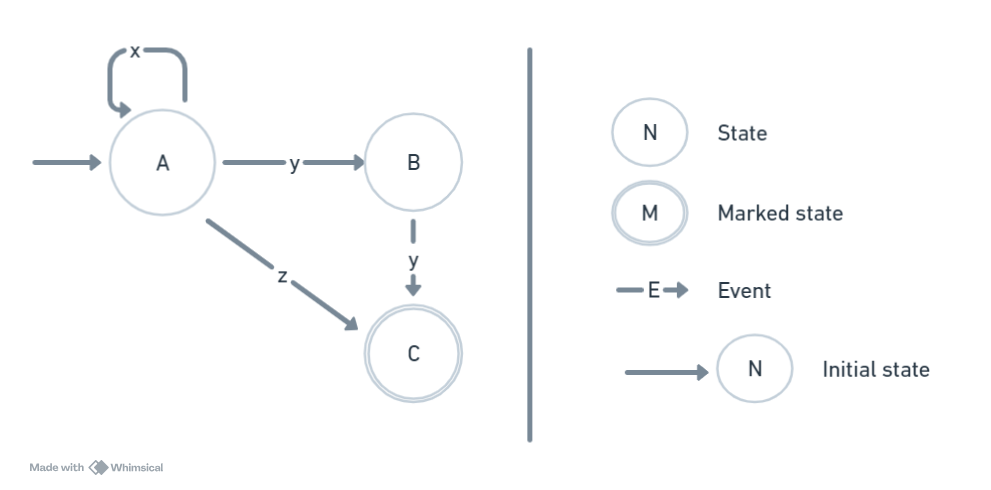
\includegraphics[width=0.7\linewidth]{figuras/automaton.png}
    \caption{State Transition Diagram example.}
    \label{fig:state_transition_diagram_example}
\end{figure}

\noindent
States:
$$
X=\{A, B, C\}
$$

\noindent
Events:
$$
\Sigma=\{x, y, z\}
$$

\noindent
State Function:
For a given state and event, the following function describes the resultant state: \(f(A, x) = A\), \(f(A, z) = C\), \(f(A, y) = B\), \(f(B, y) = C\), \(f(B, x)\) is undefined, \(f(B, z)\) is undefined, \(f(C, x)\) is undefined, \(f(C, y)\) is undefined, and \(f(C, z)\) is undefined.


\noindent
Active Event Function:
This function specifies which events are possible in a particular state:
\[
\Gamma(A) = \{x, y, z\}, \quad \Gamma(B) = \{y\}, \quad \Gamma(C) = \{\}
\]

\noindent
Initial State:
$$
x_0=A
$$

\noindent
Marked States:
$$
X_m=\{C\}
$$

\paragraph{} Figure \ref{fig:state_transition_diagram_example_with_lock} exemplifies the behaviors of locks within state machines, particularly focusing on deadlock and livelock situations. The automaton \(G\) for this figure can be defined as: $G = \left(X, \Sigma, f, \Gamma, x_0, X_m\right)$ where:

\begin{itemize}
  \item \(X = \{A, B, C, D, E, F\}\) is the set of states.
  \item \(\Sigma = \{x, y, v, w, z\}\) is the finite set of events.
  \item \(f: X \times \Sigma \rightarrow X\) is the state transition function, defined by:
  \[
  f(A, x) = A, \quad f(A, y) = B, \quad f(A, v) = F, \quad f(A, w) = D, \quad f(A, z) = C,
  \]
  \[
  f(B, y) = C, \quad f(D, v) = E, \quad f(D, z) = E
  \]
  \item \(\Gamma: X \rightarrow 2^{\Sigma}\) maps each state to the set of viable (active) events, defined as:
  \[
  \Gamma(A) = \{x, y, v, w, z\}, \quad \Gamma(B) = \{y\}, \quad \Gamma(C) = \{\}, \quad \Gamma(D) = \{v, z\},
  \]
  \[
  \Gamma(E) = \{\}, \quad \Gamma(F) = \{\}
  \]
  \item \(x_0 = A\) is the initial state.
  \item \(X_m = \{C\}\) is the set of marked states.
\end{itemize}


\begin{figure}[H]
    \centering
    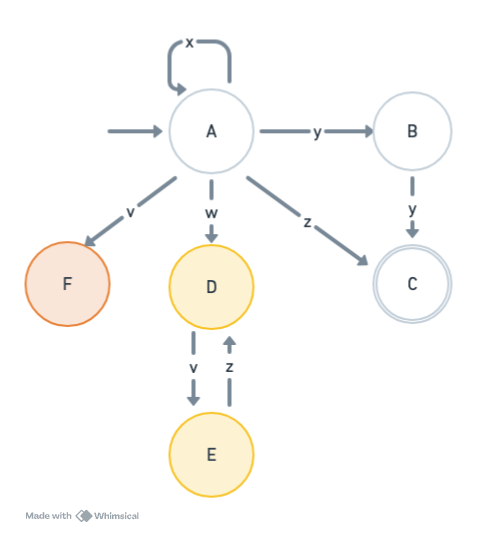
\includegraphics[width=0.5\linewidth]{figuras/automaton_lock.png}
    \caption{State Transition Diagram example with locks.}
    \label{fig:state_transition_diagram_example_with_lock}
\end{figure}

\paragraph{} State F represents a deadlock condition, characterized by the absence of any possible events that could trigger a transition from this state. Once reached, the system remains indefinitely in this state, unable to progress to a marked state. States D and E together demonstrate a livelock scenario. While there are events that transition the system between these two states, no event leads to a marked state.

\paragraph{} A system experiences a blocking when the following condition is met:
$$
\overline{L_m(G)} \subset L(G)
$$
\noindent
Conversely, there is no blocking within the system when:
$$
\overline{L_m(G)}=L(G)
$$



\paragraph{} The generated language \(L(G)\) includes: \(x^n\) (staying in \(A\) via \(x\)), \(x^n y\) and \(x^n y y\) (from \(A\) to \(B\) and then to \(C\)), \(x^n z\) (from \(A\) to \(C\)), \(x^n v\) (from \(A\) to \(F\)), \(x^n w v\) (from \(A\) to \(D\) to \(E\)), \(x^n w v z\) (from \(A\) to \(D\) to \(E\) and back to \(D\)). It can also loop between \(D\) and \(E\). Hence:
\[
L(G) = \left\{ x^n, x^n y, x^n y y, x^n z, x^n v, x^n w, x^n w v, x^n w v z, x^n w v z v, x^n w v z v z ... \mid n \geq 0 \right\}
\]
The marked language \(L_m(G)\) consists of strings that end in the marked state \(C\):
\[
L_m(G) = \left\{ x^n y y, x^n z \mid n \geq 0 \right\}
\]
The prefix-closure \(\overline{L_m(G)}\) includes all prefixes of strings in \(L_m(G)\):
Prefixes of \(x^n y y\): \(\left\{ \epsilon, x, x^2, \ldots, x^n, x^n y, x^n y y \right\}\)
Prefixes of \(x^n z\): \(\left\{ \epsilon, x, x^2, \ldots, x^n, x^n z \right\}\)
Thus:
\[
\overline{L_m(G)} = \left\{ x^m, x^m y, x^m y y, x^m z \mid m \geq 0 \right\}
\]
Checking for locks using the conditions provided:
Lock Condition: \(\overline{L_m(G)} \subset L(G)\)
\[
\overline{L_m(G)} = \left\{ x^m, x^m y, x^m y y, x^m z \mid m \geq 0 \right\}
\]
\[
L(G) = \left\{ x^n, x^n y, x^n y y, x^n z, x^n v, x^n w, x^n w v, x^n w v z, x^n w v z v, x^n w v z v z ... \mid n \geq 0 \right\}
\]
Since \(\overline{L_m(G)}\) does not include strings with \(v\), \(w v\), or \(w v z\), and these strings are part of \(L(G)\), it is evident that:
\[
\overline{L_m(G)} \subset L(G)
\]

\noindent
Given that \(\overline{L_m(G)}\) does not include all strings from \(L(G)\), the condition \(\overline{L_m(G)} = L(G)\) is not met.



% ---------------------------------------------------------------
% Chapter 3 - Conclusões
% ---------------------------------------------------------------
\chapter{Implementation}
\label{cap3}
\section{Data exchange across CERN systems} 

\paragraph{} The Glance systems are pivotal in managing CERN's detectors' projects, aiding in the creation of scientific papers, authorship attribution, and detailing the operational aspects and infrastructure of the detectors. Other CERN systems address different collaboration facets, often overlapping with Glance system data, most often Members and Employments information. This led to other groups seeking data integration with the Glance Team, initially resolved by granting read-only database access. However, this solution was fraught with challenges, especially when database modifications impacted other dependent systems. The situation became even more complex with the introduction of General Data Protection Regulation (GDPR) by the EU. According to the European Commission website \cite{eu_data_protection_explained}, this regulation safeguards the personal information of individuals within the European Union (EU) and the European Economic Area (EEA). It empowers individuals to control their data, requiring organizations to be transparent about its collection, use, and sharing. Additionally, organizations must implement security measures to protect the data. This regulation not only empowers individuals but also protects them from privacy violations and creates a level playing field for businesses operating within the EU and EEA, which includes CERN as the research center is co-hosted by France and Switzerland. GDPR is implemented through the CERN's Operational Circular no. 11 (OC11) \cite{cern_oc_11}: a document designed to ensure the protection and secure handling of personal data within the organization, in line with legal requirements and best practices. It details the principles and obligations of data processing at CERN, emphasizing the need for data security, transparency, and respect for individual rights. The document outlines the roles and responsibilities of various stakeholders, including data controllers and processors, and specifies the procedures for managing data access, consent, rectification, deletion, and portability. It also includes guidelines for data transfer outside the organization, addressing both internal and external compliance. Additionally, it establishes mechanisms for reporting data breaches and handling complaints, ensuring a structured response to potential data protection issues. 

\paragraph{} A key aspect of OC11 is the obligation imposed on Data  Controlling Services (such as the Membership) to establish one or more Records of Processing Operations relating to the Personal Data it
processes. According to \cite{cern_oc_11}, the Record of Processing Operations shall contain at least all of the following information:
\begin{enumerate}
    \item The type(s) of Personal Data being processed;
    \item The purpose of its collection;
    \item The period for which it is retained;
    \item Where applicable, details regarding use of automated decision-making; and
    \item \textbf{Where applicable, details regarding transfers of Personal Data. This may include defining all CERN Services / user groups that would consume the data provided by the Controlling Service.}
\end{enumerate} 

The last provision posed a significant challenge for the conventional practice of data sharing through database views, as it was difficult to ascertain or regulate the specific accounts granted access to these views. Therefore, to facilitate data exchange and mitigate issues of data redundancy and inconsistency and comply with OC11, Glance followed the approach chosen by other software groups to develop a REST API for the systems, allowing proper integration with other services and tools. This approach is also aligned with CERN's authentication/authorization (authz) provider, which had just started to provide OAuth 2.0 authorization endpoints. The adoption of Backend APIs also opened possibilities for developing web applications with distinct backend and frontend components and increased data restriction granularity.

\paragraph{} REST APIs serve as a set of protocols and standards used for designing networked applications. They enable systems to communicate over the internet by utilizing HTTP requests to create, read, update, and delete data, thereby facilitating interaction between client and server. A REST API abstracts the complexity of internal systems, presenting a simple, uniform interface to external entities. It operates on a stateless, client-server, cacheable communications protocol, where each request from a client contains all the information the server needs to fulfill the request. REST APIs use standard HTTP methods, such as GET, POST, PUT, and DELETE, to interact with resources, which are identified via URLs. These APIs are designed around the concept of resources, with each resource being accessed through its URI and manipulated using the HTTP methods. 

\paragraph{} Tools like the Slim Framework are used to simplify the development of web applications and APIs, particularly RESTful APIs. Slim is a PHP micro-framework that provides developers with a set of tools to build web applications and APIs quickly and efficiently. It is designed to be lean and agile, enabling developers to add only the components and functionalities they need, thereby avoiding unnecessary overhead. Slim's architecture is built around the request-response model, being used for developing REST APIs that require efficient routing, middleware support, and easy handling of HTTP requests and responses. 

\paragraph{} Middlewares, are components that intercept incoming requests or outgoing responses. They act as a layer between the request and the response or between different components of an application. Middlewares can be used for a wide range of purposes, such as authentication, logging, CORS (Cross-Origin Resource Sharing) handling, caching, and more. They allow developers to encapsulate common features in a reusable way, applying them across various routes or endpoints in the application. This makes it easier to manage cross-cutting concerns like security and performance optimizations without cluttering the core business logic of the application. Middlewares can be stacked or chained, meaning a request can pass through multiple middlewares in sequence before reaching the final route handler, allowing for modular and flexible application design.

\paragraph{} The FENCE REST API (FRAPI) was introduced to easy REST API creation. Inspired by the Slim Framework, it implements the core functionality to handle request routing to backend controller classes' methods according to predefined configurations. It also implements the all the middlewares required for a web application in the CERN context, which are: 


\begin{itemize}
    \item \textbf{Authentication Middleware}: Verifies the identity of users or systems, ensuring that only authorized entities can access the application.
    \item \textbf{Authorization Middleware}: Determines the access rights of authenticated users, restricting actions and resource access based on predefined permissions. This is particularly important for OC 11 compliance.
    \item \textbf{Request Validation Middleware}: Ensures the integrity and validity of incoming requests by checking their structure, parameters, and data formats.
    \item \textbf{Cross-Origin Resource Sharing (CORS) Middleware}: Manages cross-domain requests, enabling or restricting resource sharing across different origins in a secure manner.
    \item \textbf{Error Handler Middleware}: Provides a centralized solution for handling errors and exceptions, improving the application's reliability and user feedback.
\end{itemize}

\section{Hexagonal architecture}
\paragraph{} The integration of FRAPI for constructing REST APIs constituted merely a segment of the overarching system design. It established the methodologies for the backend to expose its functionalities and data without enforcing specific design patterns. This flexibility enabled developers to explore various architectural frameworks, ultimately converging on two predominant models: Layered Architecture and Hexagonal Architecture. This approach facilitated a comprehensive evaluation and selection of architectural patterns that best suited the project's requirements, allowing for a tailored and effective system architecture. Initial experimentation with Layered Architecture indicated its appropriateness for straightforward and smaller-scale applications. This model organizes classes based on their technical roles rather than their business functions, also promoting a database-centric design philosophy. It encourages the creation of classes that mirror the structure of a database, rather than designing to achieve specific behavioral outcomes that facilitate real-world processes. These considerations, particularly the emphasis on database-driven design and the lack of focus on business-centric modeling, steered the development team towards the other option.

\paragraph{} Hexagonal Architecture, introduced by Alistair Cockburn in 2005 \cite{cockburn2005hexagonal}, is a software architecture designed to achieve certain goals, emphasizing the isolation of business logic from external interfaces and infrastructure. This architecture aims to make the application equally controllable by users, other applications, or automated tests without the business logic being aware of the invocation source. It also seeks to enable the development and testing of business logic in isolation from databases and other infrastructures, facilitating infrastructure modernization without adjusting the business logic.

\paragraph{} The architecture is characterized by its use of ``ports" and ``adapters" to separate the business logic (the application core) from external components. The business logic defines interfaces (ports) for communication with the outside world and implements use cases exclusively against these port specifications, remaining agnostic to the technical details behind these ports. Ports serve as gateways for the application to interact with the external world, including user interfaces, APIs, databases, and other external systems. Adapters act as intermediaries, translating between the external world and the application's ports. They can be designed for various external components, allowing for flexibility in how the application interacts with different technologies and infrastructures.
The architecture distinguishes between ``primary" (or ``driving") and ``secondary" (or ``driven") ports and adapters, based on whether they control the application or are controlled by it. This distinction helps organize the flow of control and data within the system.

\paragraph{} The Dependency Rule ensures that dependencies flow inward towards the application core, preventing the business logic from being coupled to external technologies and frameworks. This supports the isolation of business logic. Dependency Inversion is a key principle in implementing secondary ports and adapters, allowing the direction of code dependencies to be opposite to the calling direction. This enables the application core to remain isolated while still interacting with external systems.

\paragraph{} In Hexagonal Architecture, the domain refers to the core business logic and data that define what the application is about. It encapsulates the business rules, entities, and logic that are central to the application's purpose.  The domain is at the heart of the architecture, as shown in red on Figure \ref{fig:hexagonal}, isolated from external concerns like UI, database access, or external service integration. This isolation ensures that changes in the external layers (like swapping out a database or changing the UI framework) do not affect the core business logic, thereby making the system more maintainable and adaptable to change. Use cases are part of the application layer that sits at the boundary of the domain (in yellow on Figure \ref{fig:hexagonal}), directly inside the ports. They define the application's available interactions in terms of the domain model, abstracting away the details of how data comes into and goes out of the system. They are the primary means by which external requests (via adapters, as illustrated in the grey section of Figure \ref{fig:hexagonal}) are translated into actions on the domain model. This could involve creating, updating, retrieving, or deleting domain entities according to the business rules. Use cases are designed to be agnostic of the external world (Figure \ref{fig:hexagonal} blue components). Whether triggered by a REST API call, a GUI action, or a scheduled job, a use case focuses solely on executing business logic.
Implementing use cases in this manner allows the domain to remain purely focused on business rules, without being tainted by concerns about how it's accessed or how its data is persisted.

\begin{figure}[H]
    \centering
    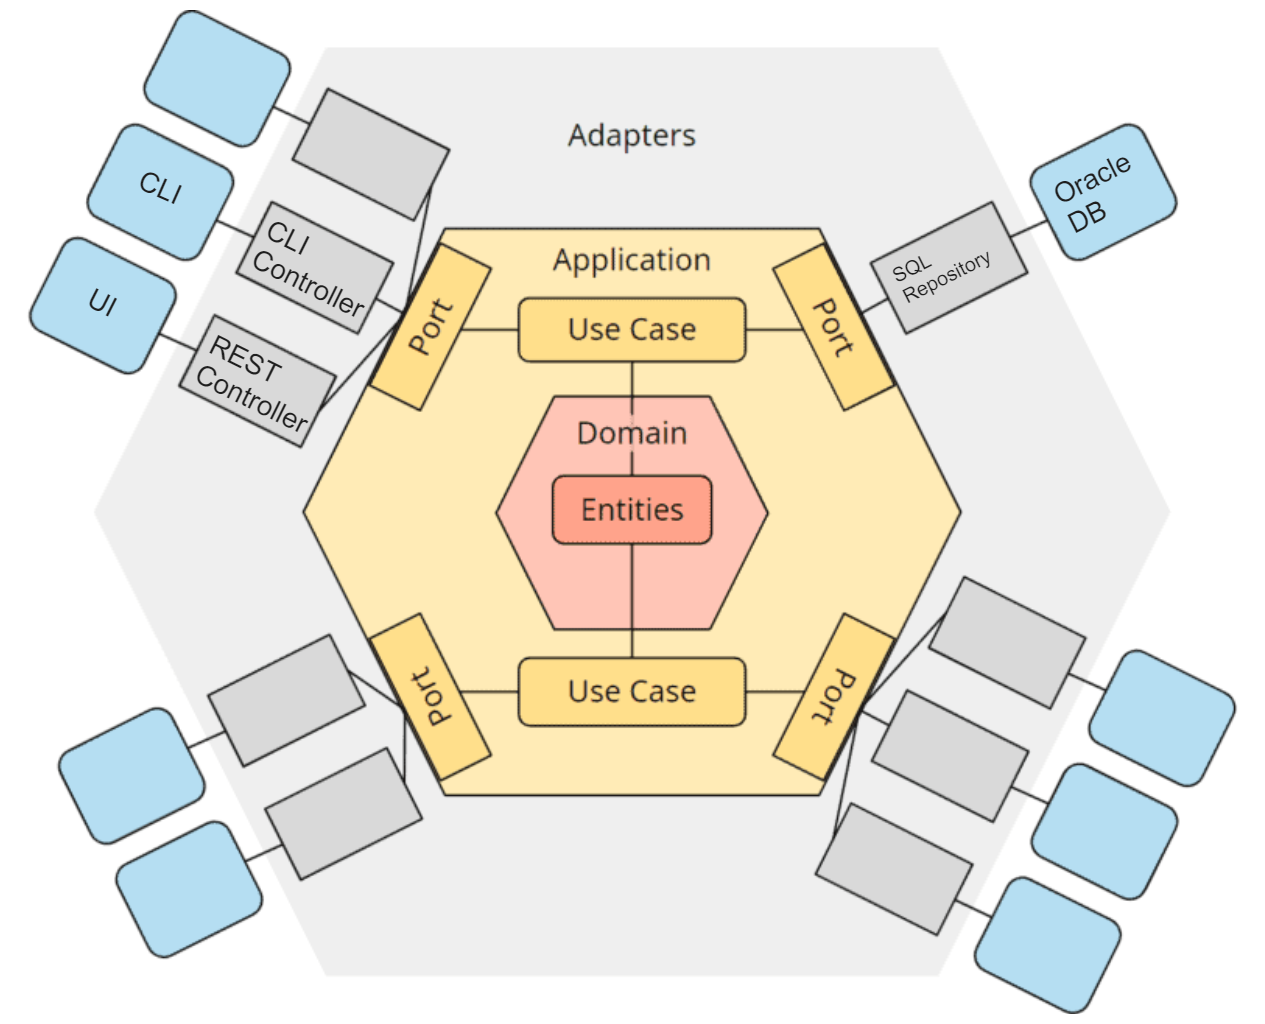
\includegraphics[width=0.8\linewidth]{figuras/hexagonal.png}
    \caption{Hexagonal Architecture visualization from \cite{happycoders2024hexagonal} adapted.}
    \label{fig:hexagonal}
\end{figure}


\section{Frontend architecture}
\paragraph{} Different from FENCE where pages were static and server-side rendered, the team decided to create single page applications (SPAs) that would consume the API endpoints exposed by the backend using FRAPI. A one-page application is a type of web application that interacts with the user by dynamically rewriting the current page rather than loading entire new pages from the server. This approach avoids interruption of the user experience between successive pages, making the application behave more like a desktop application within a web browser \cite{Adobe2023SPAs}.

\paragraph{} In a single-page application, all necessary HTML, JavaScript, and CSS code is either retrieved with a single page load or the appropriate resources are dynamically loaded and added to the page as necessary, usually in response to user actions. The page does not reload at any point in the process, nor does control transfer to another page, although modern web technologies (like HTML5 History API) allow the pages' URL to change without a full page refresh. Single-page applications (SPAs) deliver a fluid user experience by enabling the dynamic updating of webpages. This is achieved through sending requests to the server to fetch data, usually in formats like JSON or XML, and then rendering this data on the client side, which significantly reduces the amount of data transferred between the server and the client, thereby enhancing performance. This client-side rendering approach not only allows for a reduction in the server's workload—since the server is only tasked with sending data in response to requests rather than generating full HTML pages—but also leads to faster server response times and scalability advantages. Reducing the server load is a key advantage for CERN systems due to the geo-distributed user base. SPAs are designed to maintain a continuous user experience by preserving the application's state within the browser, enabling users to experience personalized content and navigate through the application without losing their current state, such as form inputs or scroll position. This stateful interaction, combined with the avoidance of full-page reloads, provides users with a fluid and app-like experience, which is especially advantageous for complex applications that feature rich interactions and workflows.

\paragraph{} Vue.js describes itself in the documentation \cite{VuejsDocumentation} as a progressive JavaScript framework used for building user interfaces chosen for the frontend architecture. It leverages standard web technologies like HTML, CSS, and JavaScript, offering a declarative and component-based programming model that facilitates the development of user interfaces, ranging from simple to complex scenarios. Vue.js is designed to enhance standard HTML with a template syntax that allows developers to declaratively specify HTML output based on JavaScript state, coupled with a reactivity system that automatically updates the DOM in response to state changes.

\paragraph{} The framework's progressive nature means it can be adopted incrementally, fitting various use cases from enhancing static HTML to powering complex Single-Page Applications (SPAs). SPAs benefit significantly from Vue.js due to its efficient update mechanisms and component-based architecture, enabling dynamic content loading and interaction without page reloads. Vue 2 uses the options API for defining component logic. This API uses a descriptive object to define state, methods, and lifecycle hooks. In Glance applications, which require a build step, components are authored using Single-File Components (SFCs). A Single-File Component in Vue.js encapsulates a component's template, logic, and styles within a single file, promoting a cohesive and modular approach to building web applications. Vue.js, coupled with its ecosystem tools such as Vue Router for client-side routing and Vuex for state management, offers a straightforward and well-documented development experience. These characteristics, along with Vue's simplicity, lightweight nature, and growing adoption—especially in comparison to heavier frameworks like React—were pivotal in the decision to utilize Vue.js for the frontend development of the new application as described by Michelly on \cite{michelly}.  

%\paragraph{} The todo list application component presented (based on \cite{vuejs2023sfc}) exemplifies the structure of a Vue.js component built with the Options API. It utilizes the BaseInputText component for the input field, allowing users to type in new todo items. Upon submission, each new item is rendered on the screen using the TodoListItem component, which displays the todo text and provides functionality to remove it from the list. This component could be integrated within a single-page application (SPA) as a route-specific view by leveraging Vue Router, Vue.js's official library for web application routing. Vue Router enables the mapping of different URLs to various components within the SPA, allowing the todo list component to be displayed when a user navigates to a specific URL, for instance, /todos. The router views are rendered in the place of a <router-view> element, and Vue Router handles the intricacies of browser history navigation and URL synchronization. Furthermore, the use of Vue's Slot API within the todo component adds a layer of flexibility, making it highly customizable. For example, by wrapping the BaseInputText with a slot, users of the todo component can replace the default input with their own customized input component or add additional HTML or Vue components around the input area. This could be particularly useful if there's a need to extend the functionality of the input, such as adding date pickers, dropdowns for categories, or tags for the todos. When discussing the Super Search implementation, the flexibility provided by slots will be leveraged to create simple and advanced search interfaces.

\paragraph{}The todo list application component, highlighted in the Vue.js script \ref{lst:vue-script} and template code \ref{lst:vue-template}, demonstrates basic use of Vue.js's Options API, integrating various features that illustrate the component's anatomy. This example is based on a live demo application provided in the Vue official documentation \cite{vuejs2023sfc}.

\paragraph{} Starting with the template structure (Vue.js template code with slot on listing \ref{lst:vue-template}), it defines the HTML markup, binding it to the Vue instance's data or methods (lines 5 to 8 of listing \ref{lst:vue-template}). The greeting message is dynamically rendered based on the computed property \verb|greetingMessage|, showcasing Vue.js's reactive data binding capabilities. The template further introduces a slot around the \verb|BaseInputText| component (Lines 4-10 of listing \ref{lst:vue-template}), enabling custom input content. This use of slots underscores Vue's flexibility and reusability, allowing developers to inject customized content or components into predefined placeholders.

\paragraph{} In the script section of \ref{lst:vue-script}, the code begins importing the \verb|BaseInputText| and \verb|TodoListItem| components (lines 2 and 3 of listing \ref{lst:vue-script}), which are required for inputting new todos and listing them respectively. This exemplifies the component-based architecture of Vue.js, where smaller, reusable components are composed to build more complex components and views. The script delineates props such as \verb|inputPlaceholder| and \verb|emptyListMessage|, which are custom attributes designed for facilitating data transfer from parent to child components. In the component illustrated in listing \ref{lst:vue-script}, the \verb|inputPlaceholder| prop is bound to the \verb|BaseInputText| component's \verb|placeholder| prop. Consequently, modifying the value of \verb|inputPlaceholder| automatically propagates the changes to the \verb|placeholder|.

\paragraph{} The data function (line 14 of listing \ref{lst:vue-script}) declares the local state of the component, including \verb|newTodoText| and \verb|todos|, illustrating the reactive state management in Vue.js. Through methods (lines 20 to 28 of listing \ref{lst:vue-script}) like \verb|addTodo| and \verb|removeTodo|, the state is manipulated, reflecting changes in the UI without direct DOM manipulation, showcasing Vue's declarative rendering capabilities.

\paragraph{}  Computed properties (line 29 of listing \ref{lst:vue-script}), such as \verb|greetingMessage|, dynamically calculate values based on reactive data, offering a cached, efficient way to update the UI based on state changes. Watchers (script \ref{lst:vue-script} line 34) on properties like \verb|todos| provide a mechanism to perform actions in response to state changes.

\paragraph{} Lifecycle hooks (script \ref{lst:vue-script} lines 39 to 44), including \verb|created| and \verb|mounted|, offer insights into the component's lifecycle stages, allowing for initialization tasks and DOM manipulations post-rendering. This demonstrates the control Vue provides over a component's lifecycle, allowing developers to hook into key events.

\paragraph{} Vue also provides tools to define scoped styles, which are applied only to the component defined in the same file as the style. This is shown in the code \ref{lst:vue-style}.

\paragraph{} Finally, an integration with Vue Router would enable this component to be part of a SPA, mapping URLs to views/components and rendering them within a \verb|<router-view>| element, facilitating SPA development with Vue.js. Vue Router's handling of browser history and URL synchronization enhances the SPA navigability and allows users to use the browser's back button. Image \ref{fig:todo-app} illustrates what the component created looks like.


\begin{lstlisting}[language=HTML, caption=Vue.js template code with slot., label=lst:vue-template]
<template>
  <div>
    <h1>{{ greetingMessage }}</h1>
    <slot name="input">
      <BaseInputText 
        v-model="newTodoText"
        :placeholder="inputPlaceholder"
        @keydown.enter="addTodo"
      />
    </slot>
    <ul v-if="todos.length">
      <TodoListItem
        v-for="todo in todos"
        :key="todo.id"
        :todo="todo"
        @remove="removeTodo"
      />
    </ul>
    <p v-else>
      {{ emptyListMessage }}
    </p>
  </div>
</template>
\end{lstlisting}


\begin{lstlisting}[language=javascript, caption=Vue.js script code., label=lst:vue-script]
<script>
import BaseInputText from './BaseInputText.vue'
import TodoListItem from './TodoListItem.vue'

export default {
  components: {
    BaseInputText,
    TodoListItem
  },
  props: {
    inputPlaceholder: String,
    emptyListMessage: String
  },
  data() {
    return {
      newTodoText: '',
      todos: []
    }
  },
  methods: {
    addTodo() {
      this.todos.push({ id: this.nextTodoId++, text: this.newTodoText });
      this.newTodoText = '';
    },
    removeTodo(idToRemove) {
      this.todos = this.todos.filter(todo => todo.id !== idToRemove);
    }
  },
  computed: {
    greetingMessage() {
      return `You have ${this.todos.length} todos`;
    }
  },
  watch: {
    todos(newTodos) {
      console.log('The todo list has changed!', newTodos);
    }
  },
  created() {
    console.log('Component has been created');
  },
  mounted() {
    console.log('Component has been mounted to the DOM');
  }
}
</script>
\end{lstlisting}

\begin{lstlisting}[language=HTML, caption=Vue.js style code., label=lst:vue-style]
<style scoped>
button {
  font-weight: bold;
}
</style>
\end{lstlisting}
\begin{figure}[H]
    \centering
    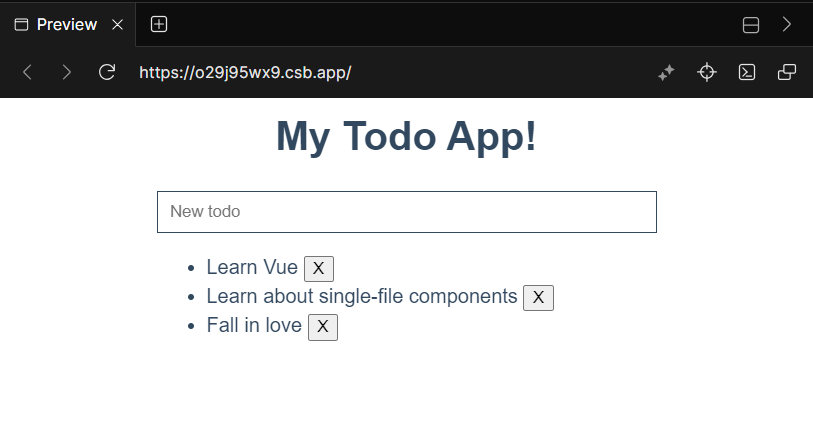
\includegraphics[width=0.8\linewidth]{figuras/todo-app.png}
    \caption{Todo Vue app example.}
    \label{fig:todo-app}
\end{figure}


%\subsection{vuex}

\paragraph{} In the project's early stages, the developers embarked on creating a suite of components that would serve as the foundational building blocks for new systems. This suite encompassed a variety of elements, such as text inputs, tables, and navigation bars, among others. Complementing these components, the team crafted a dedicated plugin to handle user authentication, all of which were consolidated into a JavaScript library named fence-vue. Despite this effort, the developers recognized the existence of numerous established libraries offering similar functionalities, moved by vast and active communities. A notable example is Vuetify—a material design UI framework built atop Vue.js. Vuetify stands out by providing an extensive array of pre-designed, customizable components and directives that expedite the process of creating aesthetically pleasing and responsive web applications. One of the significant benefits of Vuetify is its integration with Figma, a web-based collaborative tool for UI/UX and graphic design that facilitates real-time teamwork. With its Figma components, Vuetify enables developers to swiftly prototype and iterate on interface designs, ensuring a smooth design-to-development workflow and fostering a more agile and collaborative environment. Figure \ref{fig:vuetify} shows some of Vuetify's components on a Figma project. The developers then limited the scope of fence-vue to common plugins and more complex components built on top of Vuetify's base ones.


\begin{figure}[H]
    \centering
    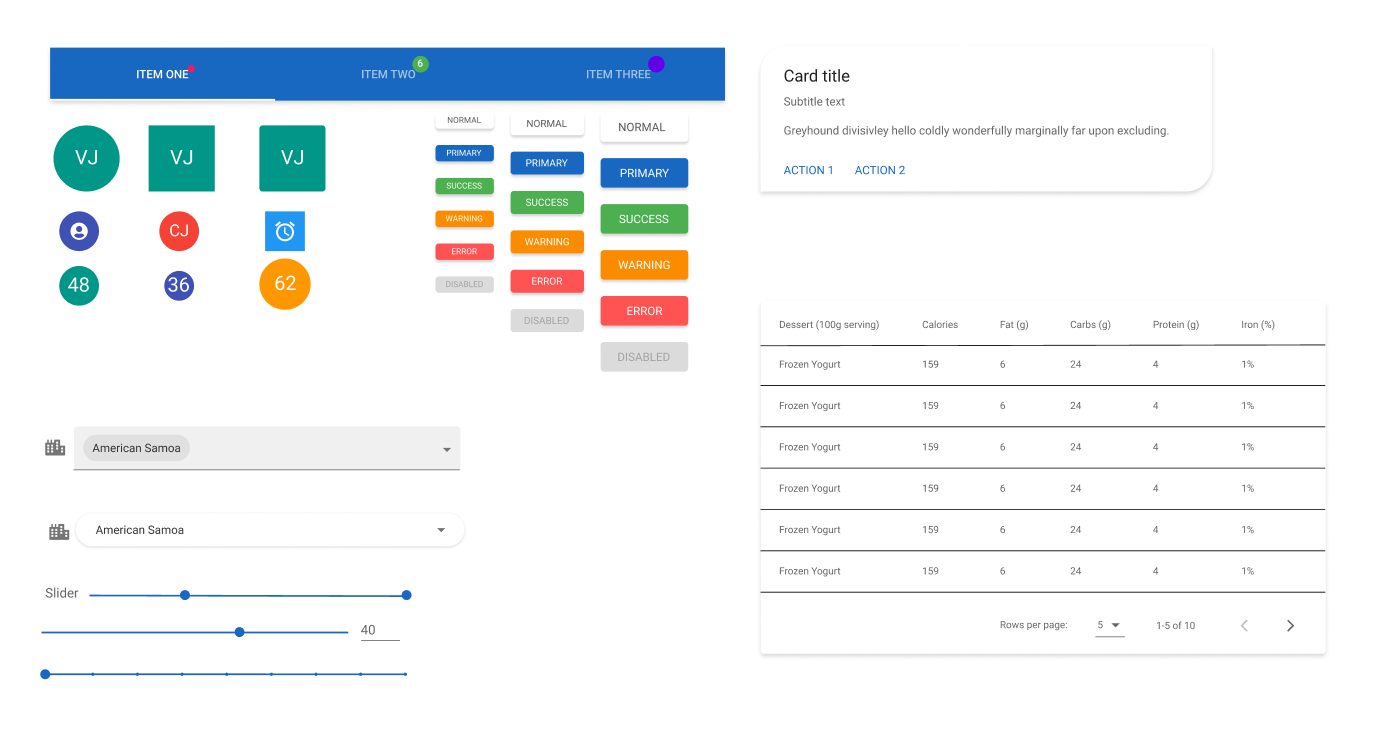
\includegraphics[width=1\linewidth]{figuras/vuetify.png}
    \caption{Some of Vuetify's components shown in Figma.}
    \label{fig:vuetify}
\end{figure}

\section{Authorship Implementation} 

\paragraph{} The Authorship implementation started at the beginning of 2020, following a consensus among stakeholders and developers that the gathered requirements were sufficiently mature. However, the development began during a period when the team was adhering to the Layered Architecture model. This timing resulted in certain inconsistencies within the system's design. Notably, newer features implemented after the initial deployment to production had already transitioned to following the Hexagonal Architecture, leading to a mix of architectural approaches.

\paragraph{} Upon starting a new project, it's necessary to register the new application on the CERN applications portal. This involves registering two separate applications: one for the frontend and another for the API, which is important for creating the needed credentials to safely communicate between the two. After registering the application, the next step is to add a new CERN SSO Registration. When doing this, developers need to keep in mind that: for client applications, they must choose the option ``my application cannot store a client secret safely" to make it a public client, which means only a Client ID will be needed. For APIs, especially if the application needs to talk to secure CERN APIs like the Authz Service API, they might need to select the option that allows generating tokens, useful for tasks such as adding or removing members from a GRoups for APPlications Authorization (GRAPPA) Group. This registration process provides the required credentials (Client ID and Client Secret) for applications to authenticate users through the OAuth 2 protocol.

\paragraph{} E-Groups serve as the foundational system at CERN for granting user access to applications through membership in various groups, integrated within the Single Sign-On (SSO) tokens. Utilized extensively within the organization, E-Groups facilitate authorization in a recursive manner, allowing a single e-group to be associated with multiple other e-groups. The GRAPPA system is introduced as a modern replacement for E-Groups, aiming to address and improve upon the limitations of the previous authorization infrastructure. In the Authorship context, for example, there is a GRAPPA Group for the LHCb Glance Developers. This group is then used to grant the \verb|admin| \textbf{role} to the developers in the application's settings. Roles can be defined on a user basis or based on Grappa groups. Another example of group is the LHCb Secretariat which grants the \verb|secretariat| role in the Membership and Authorship systems.

\paragraph{} The general application folder structure has three main directories:
\dirtree{%
.1 api.
.1 client.
.1 database.
}

The \verb|api| directory houses the entire backend codebase, predominantly comprised of PHP classes. This structure facilitates the separation of concerns by ensuring that all server-side logic and data manipulation tasks are centrally managed. Conversely, the \verb|client| directory is dedicated to the frontend development aspects, encompassing Components, views, and styles to create user interfaces. Additionally, the \verb|database| directory contains SQL migration files, which play an important role in managing database schema changes and ensuring data consistency across different stages of the application's lifecycle.

\subsection{The Authorship Backend}

\paragraph{} FRAPI-based applications tend to have a similar backend structure. Expanding the \verb|api| folder content, the following subfolders can be found:

\dirtree{%
.1 api.
.2 configuration.
.2 routes.
.2 docs.
.2 resources.
.3 notifications.
.3 templates.
.3 queries.
.4 delete.
.4 insert.
.4 select.
.4 update.
.3 schemas.
.2 src.
.3 AuthorsList.
.4 Application.
.5 DeleteAcknowledgement.
.5 DeleteFundingAgency.
.5 GetAcknowledgementTex.
.5 GetAuthorsList.
.5 GetFundingAgencyDetails.
.5 GetGrantDetails.
.5 GetInternationalOrganizationDetails.
.5 RegisterAcknowledgement.
.5 RegisterAuthorsListForPaper.
.5 RegisterFundingAgency.
.5 RegisterGrant.
.5 Subscribers.
.5 UpdateGrant.
.4 Domain.
.5 Event.
.4 Infrastructure.
.4 Cronjob.
.4 Persistence.
.4 Web.
.3 Controllers.
.3 Cronjob.
.3 DTO.
.3 Models.
.3 Persistence.
.3 Notifications.
.3 Repositories.
.3 Services.
.3 tests.
.4 Comparison.
.4 Integration.
}

\paragraph{} Inside the \verb|configuration| folder, it is required to add an \verb|api.json| configuration file. This file includes authentication settings, such as defining which SSO provider will be used by FRAPI and the API public endpoints' paths.

\paragraph{} SSO is an authentication process that allows a user to access multiple applications or systems with one set of credentials, thus eliminating the need to log in separately to each system. SSO can be implemented using various authentication protocols, including SAML (Security Assertion Markup Language), OAuth, and OpenID Connect. At CERN, OAuth 2 was the protocol used provided by Keycloak: an open-source Identity and Access Management solution developed by Red Hat.


\paragraph{} In the \verb|api.json| it is also included the path for the User class, which defines a set of properties required for every authenticated user to record the actions performed by them and perform authorization checks. For the Authorship and the Membership the User class has the following properties: \verb|$id|, \verb|$appointments|, \verb|$primaryEmployment|, and \verb|$cernId|.

\paragraph{} In this file it is also provided the Sentry instance URL in case the application has one. Sentry is an open-source error-tracking software that provides monitoring and fixing of crashes in real time. It enables the detection, understanding, and resolution of issues affecting the user experience through detailed error insights. Sentry facilitates the identification of the specific line of code causing an issue, the conditions under which the error occurred, and its impact on users. This capability assists developers in addressing problems promptly, potentially before users notice them.

\paragraph{} Within the \verb|configuration\routes| directory, each API endpoint is mapped to its corresponding controller method handler. This directory contains a JSON file for each resource, which is read by FRAPI. It subsequently manages the routing of requests to the appropriate controller methods based on this configuration. As shown in the JSON \ref{lst:AuthorsListRoute} line 13, it is possible to provide an array of roles required to access a given resource. If the user tries to access a resource without the correct permission, FRAPI will return a response with HTTP status code 401: unauthorized.

\paragraph{} FRAPI also implements a middleware for JSON schema validation which ensures JSON documents (in the REST API context, the request body) adhere to a predefined structure, defined by a JSON Schema. This includes constraints on data types, properties, and formats. The schema, written in JSON, specifies properties, required fields, value constraints, and array items, among other rules. Validation occurs at runtime, safeguarding against errors and vulnerabilities by verifying data conformity. When the payload received does not pass the schema validation, FRAPI will automatically respond with a 400 Bad Request error indicating a problem with the client's request to the server specifying which fields did not pass the schema validation.

\paragraph{} The \verb|authorization| field (code \ref{lst:AuthorsListRoute} line 8) is used to provide the list of required groups a user must belong to in order to access the given endpoint.

\paragraph{}

\begin{lstlisting}[language=javascript, caption=authors list resource routes., label=lst:AuthorsListRoute]
{
    "type": "controller",
    "class": "\\LHCb\\Membership\\Controllers\\AuthorsListController",
    "paths": {
        "/authors-lists": {
            "GET": {
                "method": "getAllAuthorslistBasicInformation",
                "authorization": ["basic-user"]
            },
            "PATCH": {
                "method": "update",
                "authorization": ["editorial-board-member"],
                "schema": "resources/schemas/authorslist-update.json"
            }
        },
        "/authors-lists/institutes": {
            "GET": {
                "method": "getAllInstitutes",
                "authorization": ["basic-user"]
            }
        }
        ...
\end{lstlisting}

\paragraph{} Inside the \verb|api/docs| folder it is stored the Swagger Documentation to facilitate external systems to connect to the APIs. Swagger, as described on \cite{SwaggerDocs}, is a toolset that supports the OpenAPI Specification (OAS) for developing APIs. It enables the description of the structure of APIs, making it possible for both humans and computers to understand the capabilities of a service without accessing its source code. Swagger facilitates the documentation, client SDK generation, and API testing by providing a specification that can be used to describe APIs. This specification is written in either YAML or JSON format and includes details such as available endpoints, operations, parameters, and responses. Swagger also supports API authentication mechanisms and the description of input and output models for API operations. The Membership API Swagger Docs is shown in Figure \ref{fig:swagger}

\begin{figure}[H]
    \centering
    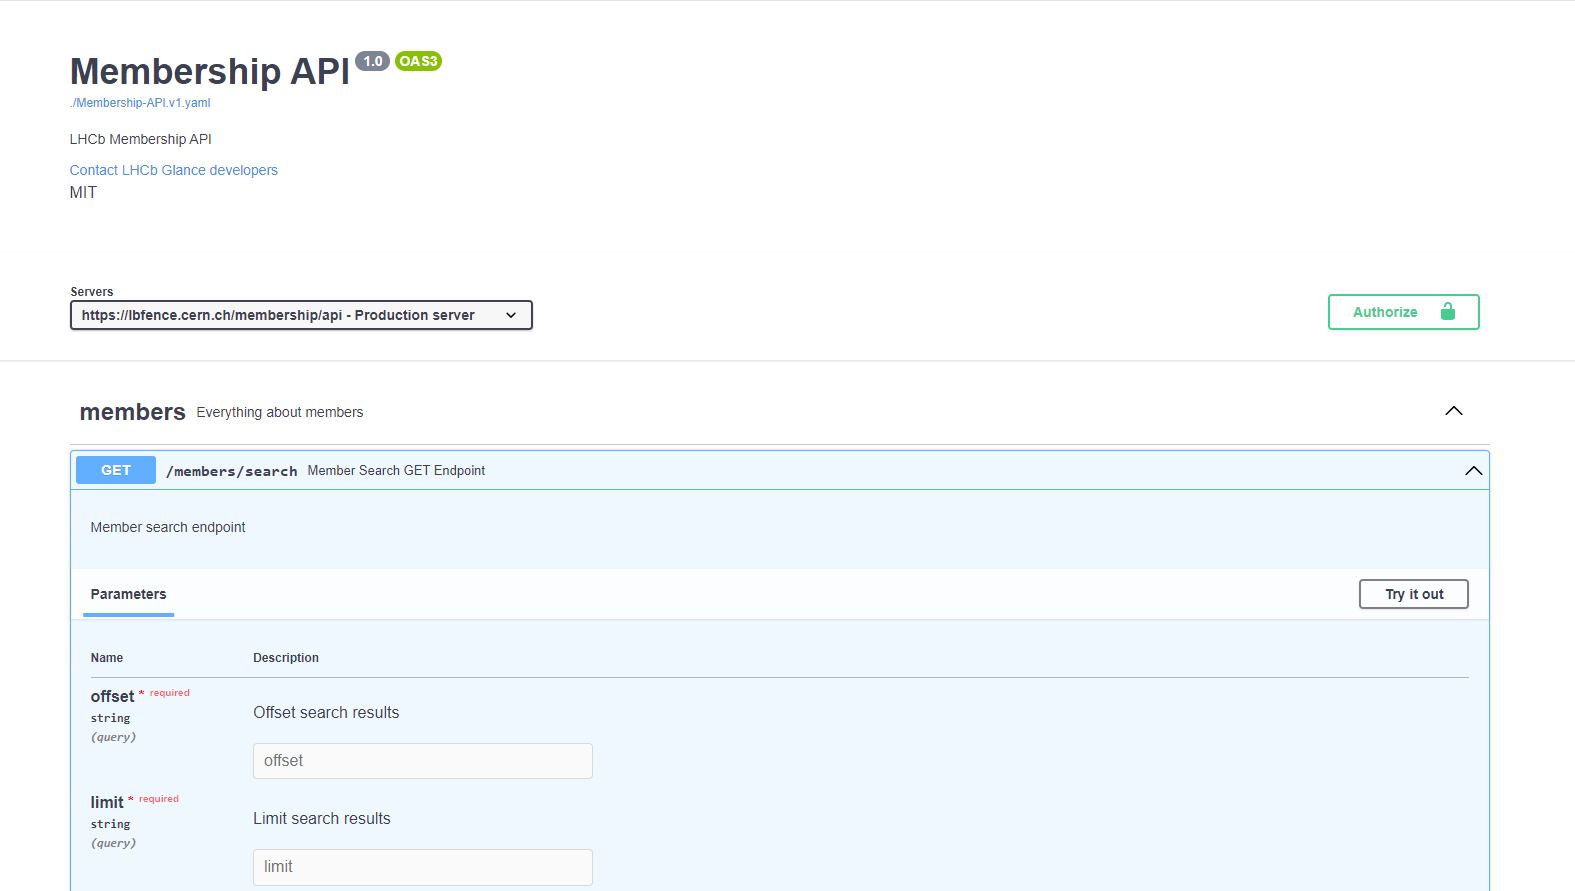
\includegraphics[width=0.8\linewidth]{figuras/swagger.png}
    \caption{API documentation example.}
    \label{fig:swagger}
\end{figure}


\paragraph{} The \verb|api/resources| directory is a repository for various non-PHP class API components. The \verb|api/resources/notifications| directory encompasses JSON configuration files that detail the subject and the corresponding HTML template for notifications. Furthermore, \verb|api/resources/templates| houses both HTML and LaTeX templates—the latter being utilized by PHP classes for generating Authorship .tex files. Additionally, the resources directory contains SQL queries employed by Repositories for database operations such as reading, writing, updating, and deleting data, as well as JSON schemas for validating request structures.

\paragraph{} The \verb|src| directory is where all PHP code within the project lives. As previously explored, the backend implementation adopts two distinct architectural patterns: the layered architecture on the left, and the hexagonal architecture on the right. The fundamental distinction between these two approaches lies in the location and application of business logic within the system's structure. Both approaches share similarities such as the Controller classes which process the request routed to them by FRAPI. They also use the Repository Pattern: a design pattern used to manage data access logic in a centralized location. It acts as an abstraction layer between the domain model (the core business logic of your application) and the persistence layer (the mechanism used to store and retrieve data, like databases or files).

\paragraph{}

\begin{minipage}{.5\textwidth}
\dirtree{% First directory structure
.2 src.
.3 Persistence.
.3 Controllers.
.3 Cronjob.
.3 DTO.
.3 Models.
.3 Repositories.
.3 Services.
}
\end{minipage}%
\begin{minipage}{.5\textwidth}

\dirtree{% Second directory structure (Duplicate of the first for demonstration)
.2 src.
.3 AuthorsList.
.4 Application.
.5 DeleteAcknowledgement.
.5 DeleteFundingAgency.
.5 GetAcknowledgementTex.
.5 GetAuthorsList.
.5 ....
.5 Subscribers.
.4 Domain.
.5 Event.
.4 Infrastructure.
.4 Cronjob.
.4 Persistence.
.4 Web.
.3 Notifications.
.3 Shared.
.4 ....
}
\end{minipage}

\paragraph{} In the Layered Architecture, the \verb|src\Controllers| directory is designated for storing Controller classes. These controllers are responsible for initiating a Data Transfer Object (DTO) when required (specifically for write or update operations) and subsequently invoking a Service class. The Service class implements the core business logic pertinent to a particular domain. The \texttt{src/Services/AuthorsList\-Service.php}, for instance, exposes a series of methods to Controllers, including but not limited to:
\begin{enumerate}
    \item \verb |getAuthorsList|: This method constructs an instance of the \path{src/Models/AuthorsList.php} class, populates it with data regarding authors and institutes, processes all the information (sorts authors, assign indexes), and delivers the assembled list back to the Controller. The Controller then serializes this list for inclusion in the response to a request.
    \item \verb|downloadAuthorsList|: Similar in functionality to \verb|getAuthorsList|, this function also compiles the authors list but differs in its output by generating a downloadable file in a specified format (e.g., PDF or .tex).
    \item \verb|insert|: This method accepts an \verb|AuthorsListInputDTO|, performs validation on it, and, if the data is deemed valid, it proceeds to persist this information through a call to the Repository dependency.
    \item \verb|getNonAuthors|: It invokes the Repository dependency to retrieve a list of members who do not qualify as authors. This functionality is particularly useful for identifying all Members eligible to be considered as exceptions.
\end{enumerate}

\paragraph{} The main issue with this approach is that the Service classes quickly grew large and became hard to maintain. This was partly caused by the fact that the classes inside the Model namespace (\verb|src/Models|) were anemic models which are considered an anti-pattern associated with object-oriented programming, particularly in the context of Domain-Driven Design (DDD) lacking significant or relevant behavior, primarily focusing on holding data with minimal or no business logic encapsulated within it.

\paragraph{} In the Hexagonal Architecture, on the other hand, there are multiple \textbf{Handler}s that process \textbf{Command}s for write operations. Controllers also have direct access to Repository interfaces so that simple operations (such as the \verb|getNonAuthors| use case) don't require a Handler for them. This approach also moves the core business logic to the Domain. In this approach, the \verb|getAuthorsList| use case starts with a request routed to a Controller method, which uses one of its N Handler dependencies, the Handler gathers all the information from the Persistence source with its Repository dependencies and supplies the \verb|\src\AuthorsList\Domain\AuthorsList| class with this information \textbf{for it to process}. Similarly, in the \verb|insert| use case, the Handler will only perform persistence-dependent validations (checking if the provided ID is unique, for example) and most of the business validation is performed in the \verb|\src\AuthorsList\Domain\AuthorsList| constructor.

\paragraph{} The following code excerpts illustrate the difference between the mentioned architectures by giving a general overview of the \verb|downloadAuthorsList| use case, which was first developed using the Layered Architecture and then migrated to the Hexagonal.

\begin{lstlisting}[language=PHP, caption={Layered Architecture Implementation.}, label=lst:layer]
// \src\Controllers\AuthorsListController.php
public function getAuthorsListForGivenPaper(Api $api, $id) {
    $authorsList = $this->authorsListService->getAuthorsList($id);
    $json = json_encode($authorsList->serialized());
    $response = $api->getResponse();
    $response->getBody()->write($json);
    return $response->withHeader("Content-Type", "application/json");
}

// \src\Services\AuthorsListService.php
public function download($id, $extension, $agentId, $date = null) {
    if ($id) {
        $authorsList = $this->getAuthorsList($id);
    } else {
        $authorsList = $this->getAuthorsListForGivenDate($date);
    }
    $data = $authorsList->serialized();
    return AuthorsListFilesHandlerService::download($extension, $data, $agentId);
}

public function getAuthorsList($id) {
    $authorsList = $this->_repository->build($id);
    if ($authorsList->hasPublishedInformation()) {
        return $authorsList;
    }
    return $this->getAuthorsListWithAssignedIndexes($authorsList);
}

private function getAuthorsListWithAssignedIndexes(AuthorsList $authorsList): AuthorsList {
    $authors = $this->getAuthors($authorsList->getReferenceDate(), $authorsList->getId());
    $institutes = $this->getInstitutes($authors, $authorsList->getReferenceDate());
    $institutes = $this->setInstitutesIndexes($institutes, $authorsList->getReferenceDate());
    $authors = $this->setAuthorsIndexes(
        $institutes["institutes-dictionary"], 
        $authors, 
        $authorsList->getReferenceDate()
    );
    $authorsList->setAuthors($authors);
    $exceptions = $authorsList->getExceptionsAuthor();
    if ($exceptions) {
        $exceptions = $this->setExceptionsIndexes(
            $institutes["institutes-dictionary"], 
            $exceptions, 
            $authorsList
        );
        $authorsList->setExceptionsAuthor($exceptions);
    }
    $authorsList->setInstitutes($institutes["sorted-institutes"]);
    return $authorsList;
}
\end{lstlisting}

In a Layered Architecture model, the interaction between the Controller and the Service layer is very close, as the latter encapsulates the majority of the application's business logic. This design paradigm often results in the consolidation of business logic within the Service layer, giving rise to voluminous, monolithic service classes. This complexity is illustrated in code \ref{lst:layer} (lines 11 to 49), where the Service initially determines whether to construct an AuthorsList for a paper or for a specific date (defaulting to the authors for the date). It then retrieves all requisite data from Repositories and processes it. This processing entails assigning indices to Institutes based on predefined rules, associating these indices with the Authors, organizing Authors and Institutes, and finally, transferring this processed data to the \verb|src/Models/AuthorsList.php| class. Rather than functioning as a domain model, this class primarily acts as a data serializer, further highlighting its anemic behavior.

\begin{lstlisting}[language=PHP, caption={Hexagonal Architecture Implementation.}, label=lst:hexagonal]
// \src\AuthorsList\Infrastructure\Web\AuthorsListController.php
public function downloadAuthorsList(Api $api, string $extension, int $id) {
    $agentId = (int) $api->getUser()->getPersonId();
    $authorsList = $this->downloadAuthorsListHandler->handle($id, $extension, $agentId);

    $response = $api->getResponse();
    $response = $response->withHeader("Content-Type", Mime::fromExtension($extension));
    $response = $response->withAddedHeader("Content-Disposition", "attachment");
    $response->getBody()->write($authorsList);

    return $response;
}

// \src\AuthorsList\Application\DownloadAuthorsList\DownloadAuthorsListHandler.php
public function handle(int $authorsListId, string $extension, int $agentId) {
    $authorsList = $this->repository->findAuthorsListById($authorsListId);
    $authorsList->computeAuthorsList();
    return AuthorsListFilesHandlerService::download($extension, $authorsList->serialized(), $agentId);
}

//  \src\AuthorsList\Domain\AuthorsList.php
public function computeAuthorsList(): void {
    $this->computeInstitutesIndexes();
    $this->computeAuthorsIndexes();
    $this->computeExternalAuthorsIndexes();
    $this->sortAllAuthors();
}
\end{lstlisting}

\paragraph{} In the code snippet (\ref{lst:hexagonal}), the distribution of tasks is optimized, facilitating a clearer comprehension of the procedure for assembling the authorship list. Similar to the Layered Architecture approach, the request navigates to the Controller via FRAPI, which now interfaces with various Handlers, such as but not limited to:
\begin{itemize}
    \item \verb|RegisterAuthorsListForPaperHandler|
    \item \verb|UpdateGrantHandler|
    \item \verb|DownloadAuthorsListForGivenDate|
    \item \verb|GetNonAuthors|
    \item \verb|RegisterAcknowledgementHandler|
\end{itemize}
\noindent
Upon receiving a request, the Controller engages the appropriate Handler to coordinate the necessary operations to address the request. As delineated in (\ref{lst:hexagonal}), the Handler employs a Repository to create an instance of the \texttt{AuthorsList} class, supplying it with all pertinent data required for the compilation of the list. This includes all Members eligible for authorship, any Exceptions (Authors added or removed), and a catalog of Institutes. Subsequently, the \texttt{AuthorsList} domain class undertakes the processing of this data, thereby consolidating all expertise related to the list's formation within the Domain. The construction of the list is executed via the \texttt{computeAuthorsList} method, which administers a series of sub-tasks to generate and structure the author roster, their affiliations, and external contributors in accordance with a set of criteria and regulations. The methodology is deconstructed into four phases, as illustrated in line 21 of code (\ref{lst:hexagonal}).

\paragraph{} The first step, performed in the \verb|computeInstitutesIndexes|, method involves assigning indexes to each Institute within the list. These indexes are necessary for organizing Institues in a structured way and for referencing them efficiently in other parts of the authors list computation. The algorithm attributes a numeric index to Official and Affiliated institutes and an alphabetical one to the others. Index attribution follows a hierarchical sorting criterion, prioritizing Country, City, and then Institute Name. This systematic ordering culminates in a structured mapping, where each institute is linked to a unique composite ID—integrating both its Id and classification (External or Regular)—and a corresponding index. This associative dictionary facilitates efficient retrieval and linkage between Institutes and their respective Authors.

\paragraph{} After institutes have been indexed, each Author's index is computed based on their Employments with these Institutes. This is first done for regular LHCb Authors (in \verb|computeAuthorsIndexes|) and later for External Authors (in the \texttt{compute\-External\-Authors\-Indexes} method). Authors may be affiliated with one or more Institutes, and their index reflects this association. The index assignment process involves iterating through each Author, determining their affiliated Institute based on the reference date, and then assigning the Institute's index to them, which is done in constant time by accessing the dictionary previously built. This step is important for organizing authors in a way that reflects their professional or academic affiliations accurately. The same process is performed for External Authors.

\paragraph{} Finally, the \verb|sortAllAuthors| function involves sorting all Authors (both internal and external) according to a predefined set of criteria, which includes the index, the alphabetical order of last names, and the initials in this order of priority. 

\paragraph{} Once the list is compiled, the Handler uses a static class (line 18 of code \ref{lst:hexagonal}) to download the serialized content into a given format (PDF, .tex, for example) and passes the content to the Controller which encapsulates it in the response object exposed to the final user through FRAPI again.

\paragraph{} Domain Classes have the capability to emit events, for instance, when a new Grant is registered, the \verb|src\AuthorsList\Domain\Event\NewGrant.php| event is emitted. These events are monitored by Subscribers, as exemplified by those located in \verb|src\AuthorsList\Application\Subscribers|. Subscribers respond to the events they receive, often by initiating notifications through the \verb|src\Notifications| classes. Employing this pattern, commonly seen in multithreaded languages such as C\#, is also beneficial in PHP to enhance the separation of concerns, delegating specific responsibilities to more specialized namespaces.

\paragraph{} The final Authorship Backend aspect are the Cronjob classes inside \texttt{src\textbackslash Cron\-job}. A cron job is a scheduled task in Unix-based systems used for running scripts or commands at specified times and intervals. It leverages the cron daemon, a background process that runs continuously, checking for scheduled tasks to execute. Cron jobs are commonly used for automating system maintenance, monitoring tasks, and routine backups. The scheduling of a cron job is defined in a cron table (crontab), which specifies the execution time and command to be run. In the Authorship context, cronjobs are used to send notifications when a Grant is about to expire. 


\paragraph{} The authorship generation process is designed to be deterministic, ensuring that identical commands (e.g., \verb|$authorsListId|) consistently produce the same author list. Due to a stringent deadline for project delivery, unit testing was not conducted. Instead, an integration test suite was developed within the \verb|src/Integration| namespace. This suite performs end-to-end testing to verify the responsiveness of all endpoints to simulated requests. Additionally, the \verb|src/tests/Comparison| namespace contains a series of end-to-end tests designed to ensure the stability of the Authors List's content amidst code changes. These tests generate the authorship list in various formats and compare the output against a predefined, accurate version. 

\paragraph{} In contrast to the FENCE applications, which lacked a clear separation of concerns, leading to the necessity of deploying applications on a testing server for manual validation of changes, the current approach allows for backend modifications to be automatically verified. This is achieved by executing the Integration test suite through the GitLab CI/CD (Continuous Integration/Continuous Deployment) tools. GitLab CI/CD provides a framework for automating the testing and deployment processes. It facilitates the execution of predefined test suites upon each commit, ensuring that any code alterations do not break the existing functionality. Figure \ref{fig:pipeline} shows a merge request that passed the integration tests. 

\begin{figure}[H]
    \centering
    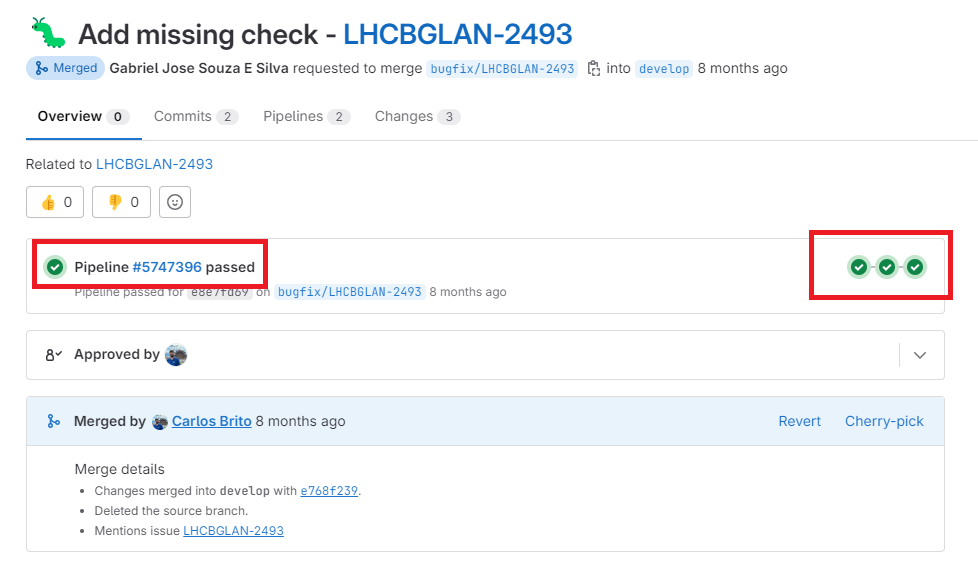
\includegraphics[width=0.8\linewidth]{figuras/tcc_pipeline.png}
    \caption{Gitlab Pipeline passing on Merge Request. The pipeline steps include building the backend API with \texttt{composer install}, building the frontend with \texttt{npm run build}, and running the backend integration test suite.}
    \label{fig:pipeline}
\end{figure}





\subsection{The Authorship frontend}

\paragraph{} The frontend of the Authorship System is housed within the \verb|client| directory. 

\dirtree{%
.1 client.
.2 public.
.2 src.
.3 api.
.3 assets.
.4 css.
.4 images.
.3 components.
.3 mixins.
.3 plugins.
.3 router.
.3 store.
.4 modules.
.3 views.
.4 authorsList.
}

\paragraph{} Within this directory, the \verb|client/public| folder contains the application's entry point HTML file, which is automatically generated by utilizing the Vue Command Line Interface (CLI) via the \verb|vue create| command. The \verb|assets| folder, also located within the \verb|client| directory, stores static assets utilized by the frontend. These assets include CSS style sheets that are applied globally across all components and static images, such as the LHCb collaboration logo and the homepage banner.

\paragraph{} The \verb|components| folder houses the fundamental building blocks of the user interface, akin to the example provided in the todo application illustrated in code \ref{lst:vue-script}. The guiding philosophy for developing components was to resort to custom creation only when the pre-existing components from Vuetify failed to meet specific needs or when it was necessary to combine several Vuetify components to build a more complex one. For instance, Image \ref{fig:tcc_latex_title} showcases a custom component designed to accept a LaTeX expression through its props and render the corresponding text. Conversely, Figure \ref{fig:tcc_loading} depicts a custom component crafted by integrating Vuetify's \verb|VDialog|, which generates the modal window, with Vuetify's \verb|VProgressLinear| to visually signify the loading process. The second one is displayed whenever a user triggers an action and the interface must wait for the response.


\begin{figure}[H]
    \centering
    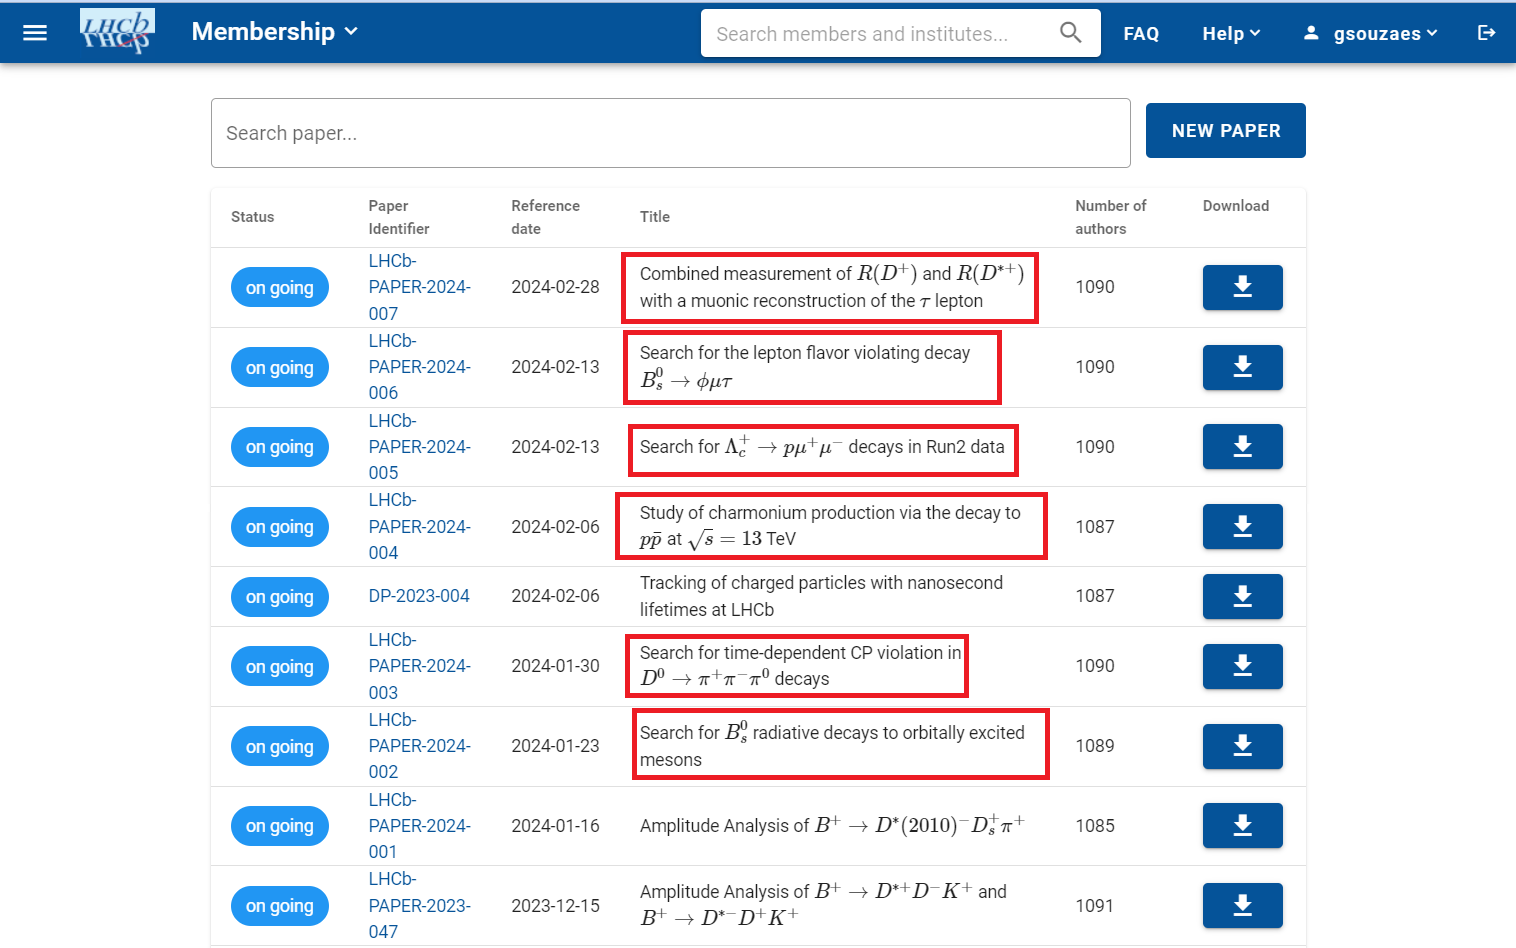
\includegraphics[width=0.9\linewidth]{figuras/tcc_authorship_home.png}
    \caption{\texttt{LatexTitle.vue}: Textual component to process latex code.}
    \label{fig:tcc_latex_title}
\end{figure}


\begin{figure}[H]
    \centering
    
\includegraphics[width=0.5\linewidth]{figuras/tcc_loading.png}
    \caption{\texttt{LoadingModal.vue}: Loading popup component.}
    \label{fig:tcc_loading}
\end{figure}

\paragraph{} Vue Mixins are stored in the \verb|client/mixins| path. A mixin object can contain any component options. When a component uses a mixin, all options in the mixin will be ``mixed" into the component's own options. This approach allows for a form of ``soft" inheritance, enabling component reuse without requiring complex inheritance structures. These scripts can include a wide range of component options such as data, methods, lifecycle hooks (e.g., created, mounted), computed properties, and watchers. When a component uses a mixin that contains a lifecycle hook, the mixin's hook is called before the component's own hook if both are defined. A very used mixin in Glance applications is shown in code \ref{lst:mailto} which injects a method in all components that import it that generates a clickable email link based on a list of emails.

\begin{lstlisting}[language=javascript, caption={Mailto Mixin.}, label=lst:mailto]
export default {
    methods: {
        getMailto(emails) {
            const localMails = !Array.isArray(emails) ? [emails] : emails;
            return `mailto:${localMails.join(',')}`;
        },
    },
};
\end{lstlisting}

\paragraph{} Inside the \verb|client/plugins| folder, the Vuetify dependency is imported. The \verb|client/router| and the \verb|client/views| folders are closely connected. In Vue.js, a view is defined in the same way as a regular SFC: a single file with a template HTML section, a script using the options API, and some custom, scoped styles if necessary. The key difference is that views can be referenced in the router configuration located in \verb|client/router/index.js|, which sets up which view will be rendered according to the typed URL. Because views are the entry points for each interface, they normally handle permissions by hiding/disabling specific components of the interface according to the user's permission. They also call store methods to fetch the necessary information to populate the interface.

\paragraph{} Vuex is a state management pattern and library designed for Vue.js applications that acts as a centralized store for all the components in an application, enforcing rules to ensure that the state can only be mutated predictably, and simplifying information sharing across multiple components.

\paragraph{} In code \ref{lst:vuex_user}, Vuex is utilized to manage user-related data within the Authorslist application. The \verb|stateData| object contains the application's state, including details such as the current user, loading status, collaboration board chair appointment ID, and lists of appointments related to the authors' list manager. This state serves as the single source of truth that can be accessed throughout the application. Getters in Vuex are similar to computed properties for components. They are used to compute derived state based on the store's state and can be used to perform operations like filtering data, calculating values, or even returning a subset of the state. For example, the code \ref{lst:vuex_user}  defines getters to check if the application is loading, retrieve user information, identify user roles and appointments, and determine if a user has administrative permissions or specific roles within the application. Actions in Vuex allow for performing asynchronous operations. They can dispatch mutations, which are synchronous transactions that directly mutate the state. In the example \ref{lst:vuex_user}, the \verb|loadUser| action fetches user data asynchronously and commits mutations to update the state based on the response. This illustrates how actions can handle complex logic, including API calls, and orchestrate multiple mutations or even other actions. Mutations are the correct way to actually change state in a Vuex store. They are synchronous and provide a clear and trackable way to modify the state. The example \ref{lst:vuex_user} includes mutations such as \verb|SET_USER| and \verb|SET_LOADING|, which update the user information and loading status, respectively. Similarly to the store module shown in \ref{lst:vuex_user}, there is another one to handle the Authors List state, which actions to fetch the list, insert exceptions, download the content, and more.

\begin{lstlisting}[language=javascript, caption={Vuex User Store Module.}, label=lst:vuex_user]
/* eslint-disable no-unreachable */
import userApi from '../../api/user';

const stateData = {
    user: null,
    loading: false,
    collaborationBoardChairAppointmentId: 13,
    authorsListManagerAppointments: [
        'Editorial board chairperson',
        'Editorial Board member',
        'Editorial board chairperson deputy',
        'Physics coordinator',
        'Physics coordinator deputy',
    ],
};

const getters = {
    loading: state => state.loading,
    user: state => state.user,
    userRoles(state, localGetters, rootState, rootGetters) {
        const simulatedRole = rootGetters['userSimulation/simulatedRole'];
        if (simulatedRole) {
            return [simulatedRole];
        }
        return state.user.roles;
    },
    userAppointments(state, localGetters, rootState, rootGetters) {
        const simulatedAppointments = rootGetters['userSimulation/simulatedAppointments'];
        if (simulatedAppointments.length > 0) {
            return simulatedAppointments;
        }
        return state.user.appointments;
    },
    userAppointmentsCategoryIds(state, localGetters) {
        return localGetters.userAppointments.map(appointment => appointment.category.id);
    },
    userIsAdmin(state, localGetters) {
        return localGetters.userRoles.includes('admin');
    },
    userIsSecretariat(state, localGetters) {
        return localGetters.userRoles.includes('secretariat');
    },
    userHasPermissionToChangeAuthorsListFlags(state, localGetters, rootState, rootGetters) {
        return localGetters?.user?.id === rootGetters['member/member']?.id
        || localGetters.userIsAdminOrSecretariat;
    },
    userHasPermissionToManagePaper(state, localGetters) {
        if (localGetters.userIsAdmin) return true;
        if (localGetters.userRoles.includes('authors-list-manager')) return true;

        if (!localGetters.userAppointments.length) return false;
        const appointments = localGetters.userAppointments.filter(
            appointment => state.authorsListManagerAppointments.includes(appointment.category.name),
        );
        if (appointments.length) return true;

        return false;
    },
   ...
};

const actions = {
    async loadUser({ commit, dispatch }) {
        let response = localStorage.getItem('membershipGetUser');
        response = response !== null ? JSON.parse(response) : null;

        if (response) {
            commit('SET_USER', response.data);
            dispatch('updateUser');
            return response;
        }

        commit('SET_LOADING', true);
        const userPromise = await userApi.getUser().then((scoppedResponse) => {
            localStorage.setItem('membershipGetUser', JSON.stringify(scoppedResponse));
            commit('SET_USER', scoppedResponse.data);
            commit('SET_LOADING', false);
        });
        return userPromise;
    },
    async updateUser({ commit }) {
        const userPromise = await userApi.getUser().then((response) => {
            commit('SET_USER', response.data);
            localStorage.setItem('membershipGetUser', JSON.stringify(response));
        });
        return userPromise;
    },
};

const mutations = {
    SET_USER(state, user) {
        state.user = user;
        state.user.name = user.fullName;
    },
    SET_LOADING(state, loadingBoolean) {
        state.loading = loadingBoolean;
    },
};

export default {
    namespaced: true,
    state: stateData,
    getters,
    actions,
    mutations,
};
\end{lstlisting}


\subsection{Database} 

\paragraph{} Once the database is created, it is modified through database migrations which are the process of applying changes or updates to a database schema—such as modifying tables, altering columns, creating indexes, or adjusting relationships between tables—as well as changes to the data within the database. The Glance team choose Flyway as the tool to manage database migrations. As described in the documentation \cite{FlywayDocumentation2024}, it is an open-source tool for database migrations that controls the process of applying and managing schema changes across different team environments, ensuring database integrity and consistency as applications evolve. It uses versioned migrations, where each script is tagged with a version number and description, to control the sequence of migration applications. The tool also employs checksums for each migration file to detect any alterations to migrations that have already been applied, thus safeguarding the migration process's integrity. Flyway tracks the state of each migration—whether pending, successful, or failed—within a designated table known as the \verb|schema_history| table, a component for identifying the migrations that have been executed and those still pending. During its operation, Flyway consults this table to determine which migrations need to be applied and proceeds to apply each in the stipulated version order. Should a migration encounter an error, Flyway halts the entire process, allowing for the issue to be resolved before moving forward.

\paragraph{} To maintain a history of data changes the team created the RFC 002, titled ``History Tables Proposal". It is an accepted proposal aiming to standardize the structure of history tables within Glance systems. It outlines several assumptions including schema separation, naming conventions, table and column inclusion, the addition of a history primary key, the exclusion of references to avoid cascade issues, and the incorporation of auditing columns for change tracking (\verb|ACTION|, \verb|AGENT_ID|, \verb|MODIFIED_ON|, \verb|DIFF_COLUMN|, \verb|OLD_VALUE| and \verb|NEW_VALUE|) in the history schema tables, which should be the same as the regular schema plus the additional columns. It also details use cases such as restoring data to a specific point in time, showcasing the practical applications of maintaining history tables for data integrity and auditing. Finally, the document specifies the implementation of triggers to automatically save changes to the history schema. These are created with a Python script that takes as input the \verb|CREATE TABLE| statements for all tables in the regular schema, and outputs a SQL file with all the necessary \verb|CREATE TRIGGER| statements.

\subsection{Functionality Summary}
Figure \ref{fig:tcc_latex_title} displays the Authorship system homepage. From it, users can select a Paper to visualize or manage its AuthorsList. The management page is shown in Figures \ref{fig:manager_paper_view_tcc} and \ref{fig:authorship_exceptions_tcc}, from this page users can add Exceptions (removing or adding Authors), export the list of Authors in different formats and layouts, register Grants and Funding Agencies to be acknowledged on a paper and mark a paper as published to prevent further modifications. The Exceptions navigation tab highlighted in Figure \ref{fig:authorship_exceptions_tcc} displays in red authors removed from the list, in blue Authors who chose to have their affiliation hidden in the list and in green an Author added to the list.

\begin{figure}[H]
    \centering
    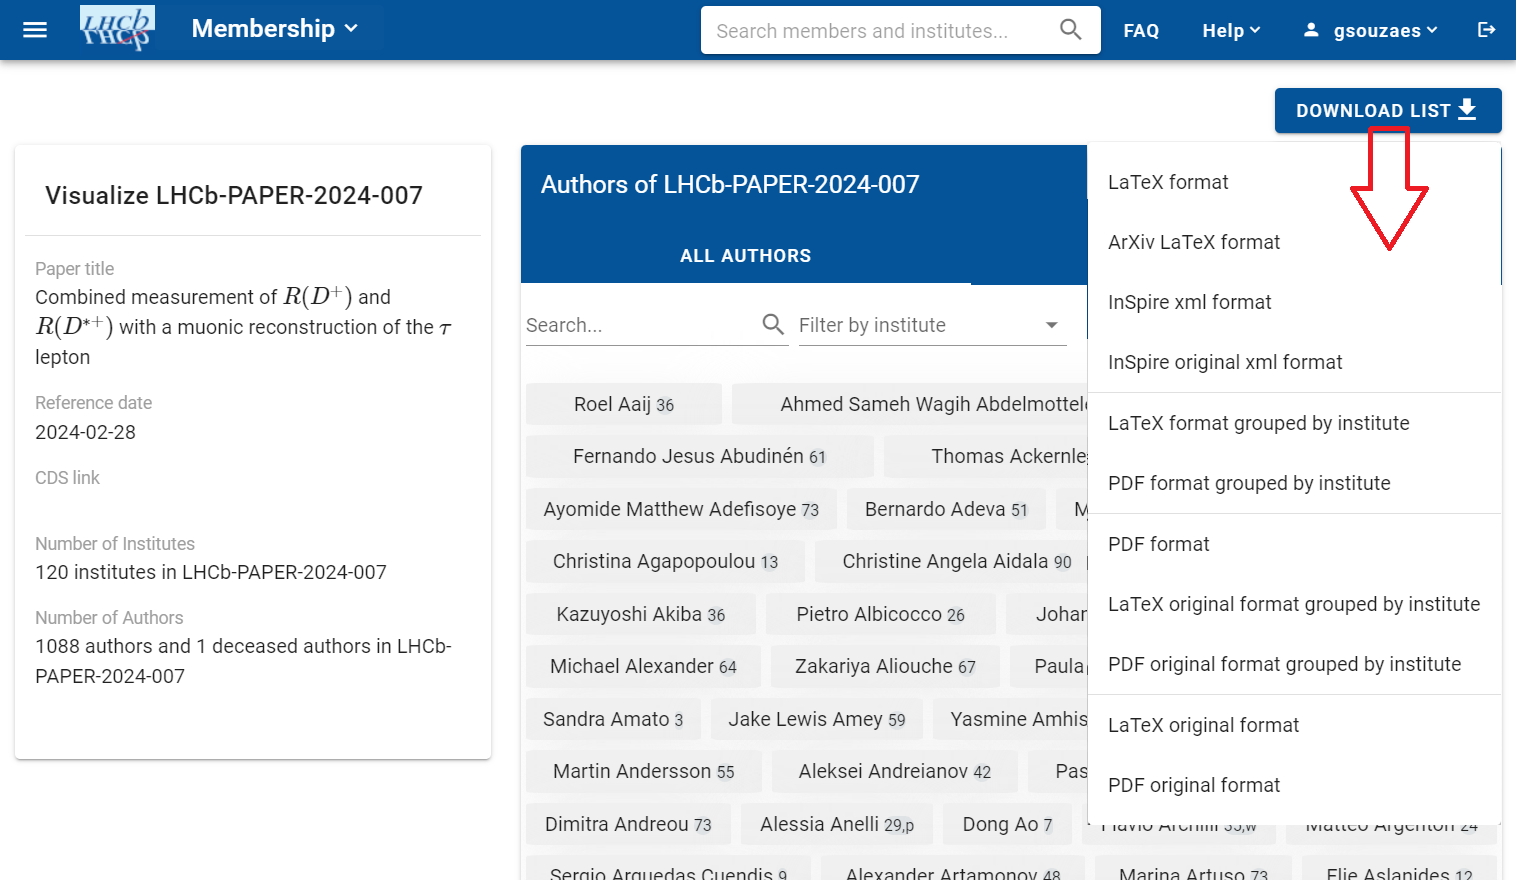
\includegraphics[width=0.8\linewidth]{figuras/manager_paper_view_tcc.png}
    \caption{Vizualize Authors List Page.}
    \label{fig:manager_paper_view_tcc}
\end{figure}

\begin{figure}[H]
    \centering
    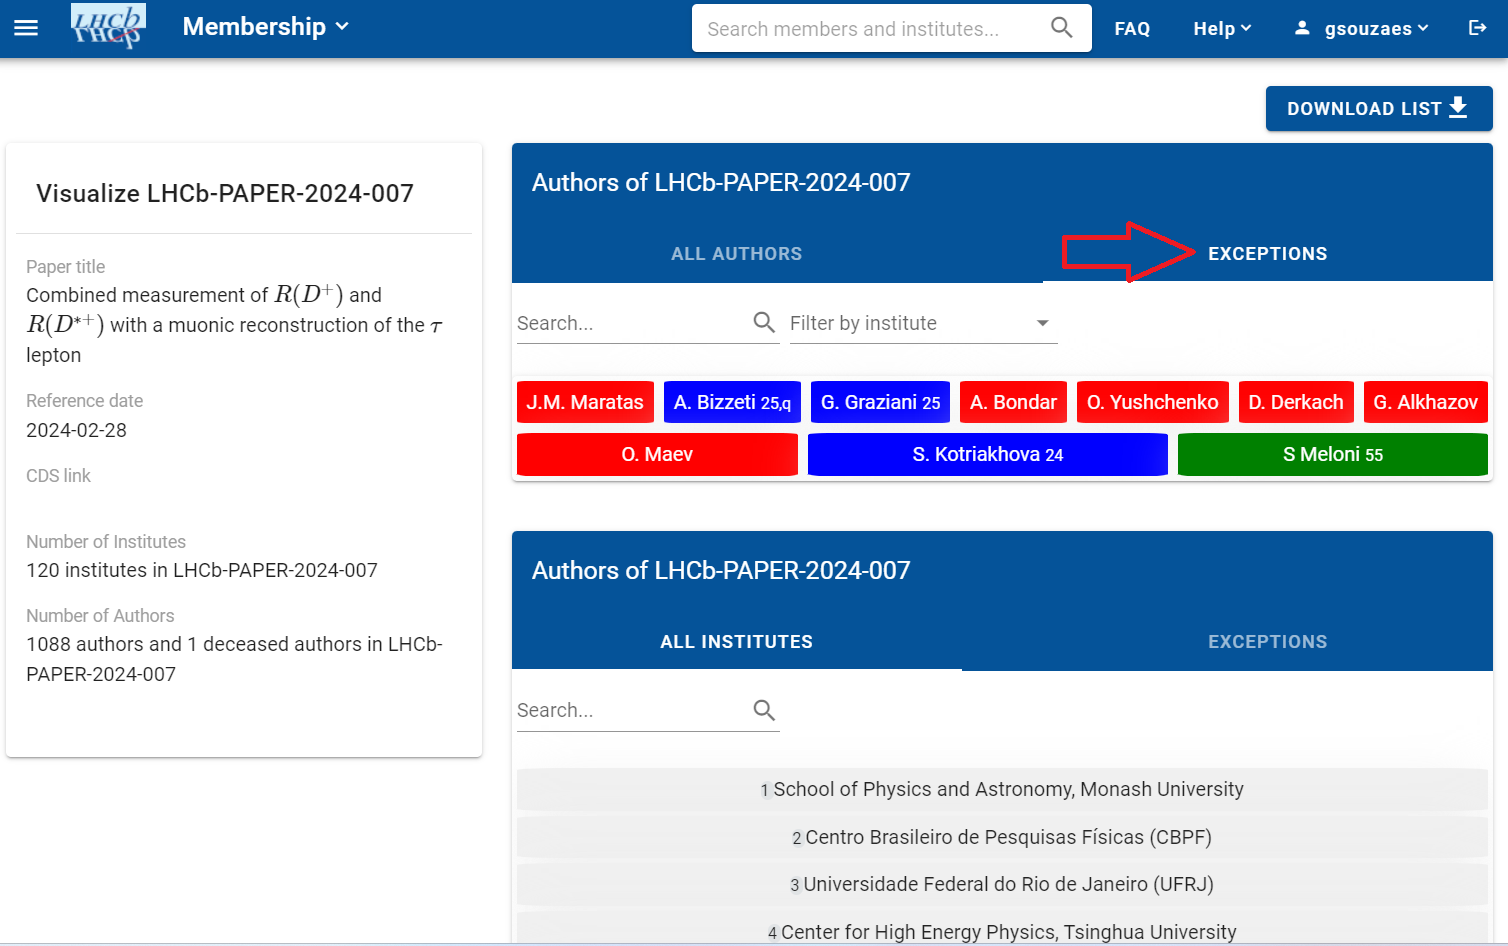
\includegraphics[width=0.8\linewidth]{figuras/authorship_exceptions_tcc.png}
    \caption{Authorship Exceptions tab.}
    \label{fig:authorship_exceptions_tcc}
\end{figure}

The two most used formats are the PDF format and the LaTeX format. This first is publicly available to expose the current list of Authors in the Collaboration and the later is usually embedded by Authors in their Papers. Figure \ref{fig:authorship_formats} displays both formats side by side. This automatic list generation is the core feature of the Authorship system, proving a reliable and standardized way for the entire Collaboration to sign a publication.

\begin{figure}[H]
    \centering
    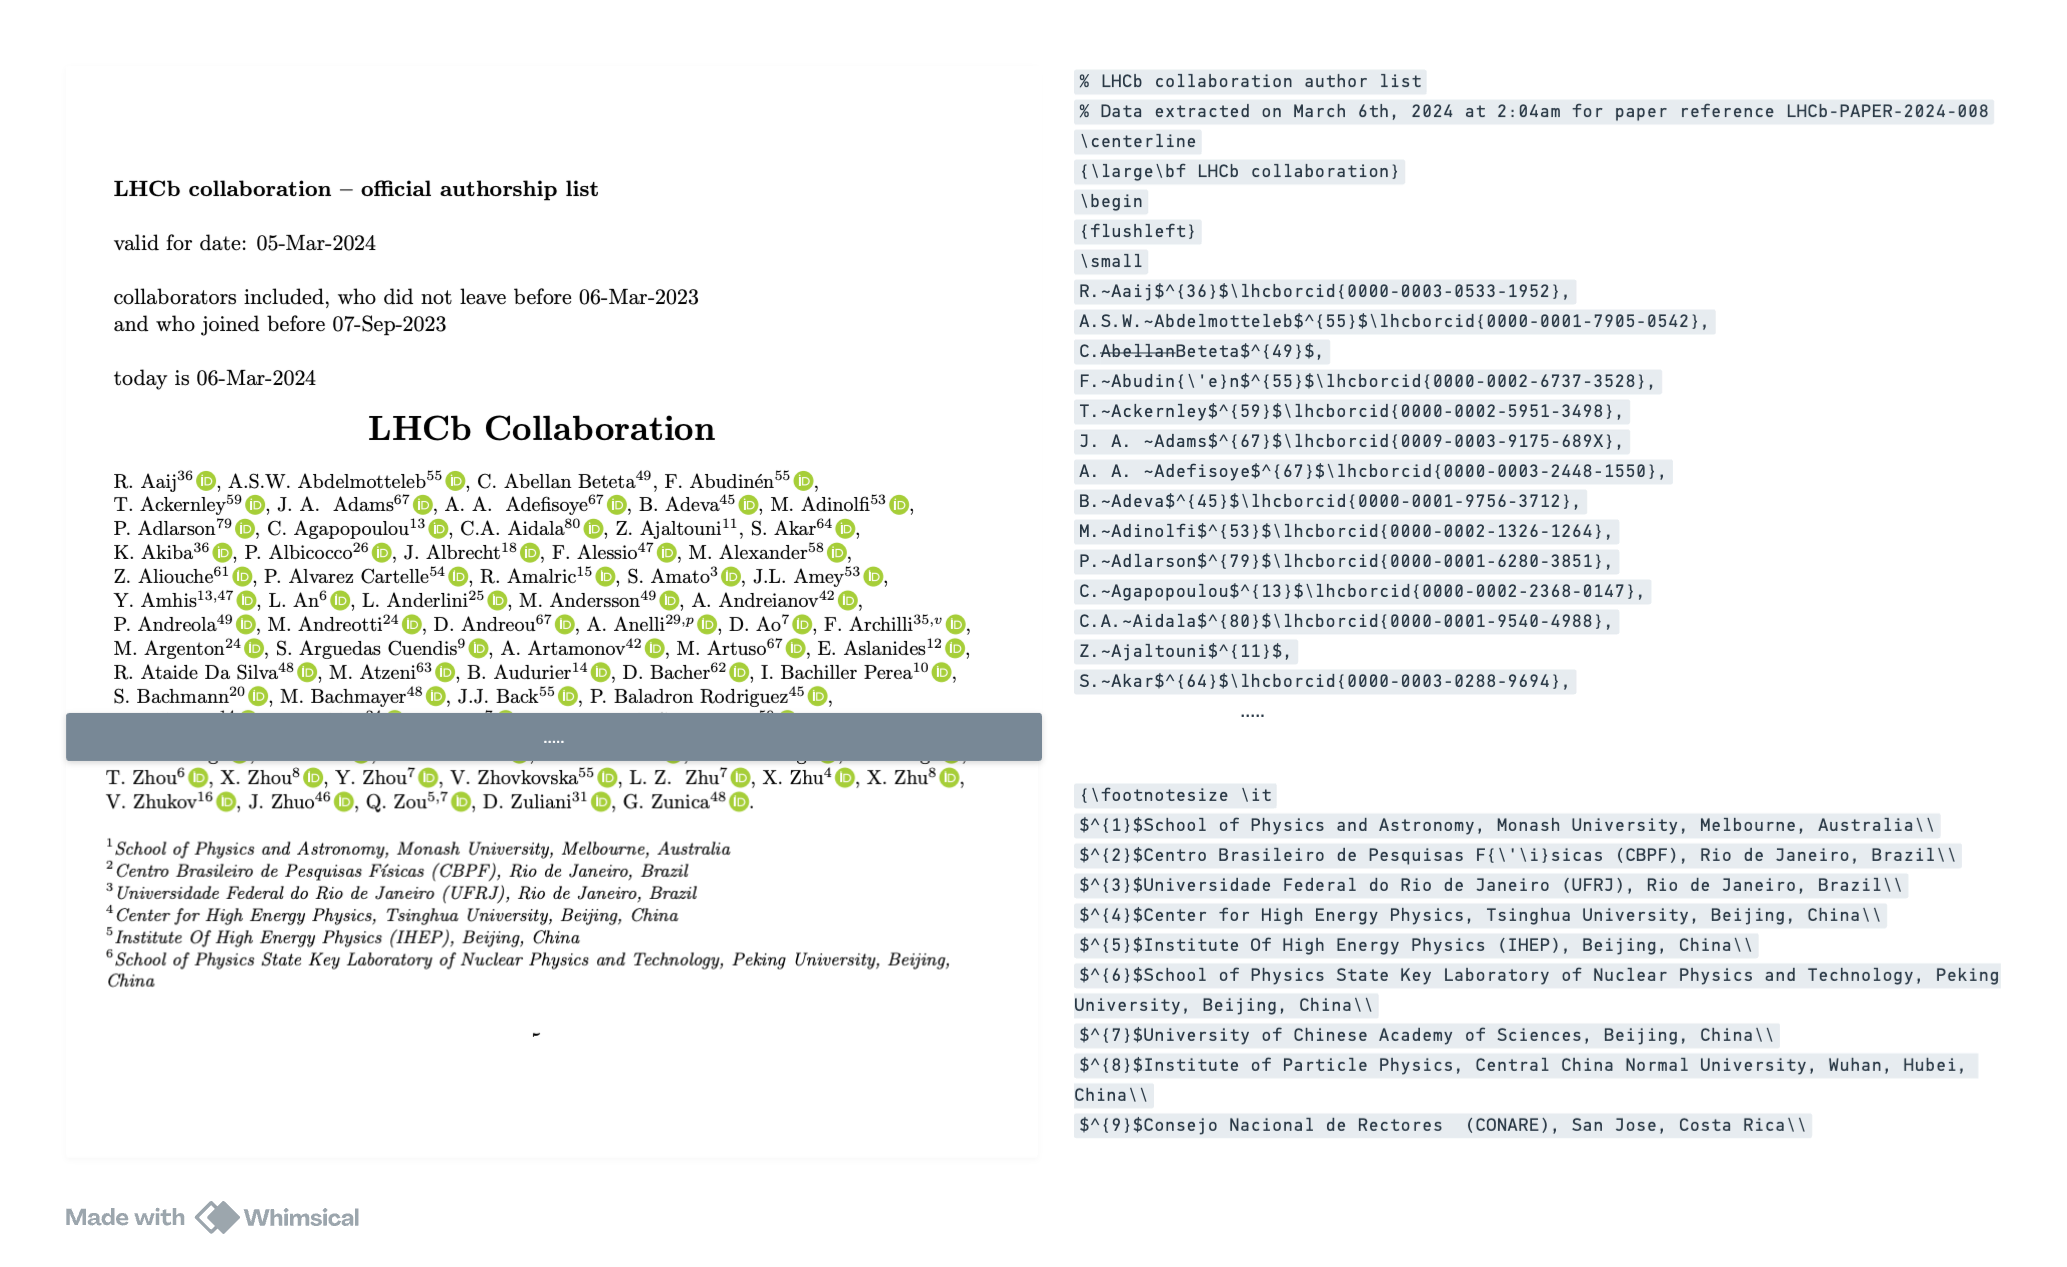
\includegraphics[width=1\linewidth]{figuras/authorship_tcc.png}
    \caption{Authorship generated files.}
    \label{fig:authorship_formats}
\end{figure}


\section{Search Implementation}  
\paragraph{} The Search Library was implemented as two different packages: a backend library for creating the search endpoints and a frontend one to provide the necessary components to build advanced search interfaces.

\subsection{Backend: search-service}

\paragraph{} The backend library is organized similarly to the backend of the Authorship web application. It also follows the Hexagonal Architecture as made explicit by the directory structure, with a Domain including classes with the knowledge to convert themselves to a piece of a SQL query.

\dirtree{%
.1 .
.2 README.md.
.2 composer.json.
.2 configuration-example.json.
.2 src.
.3 Application.
.4 DeleteSearch.
.5 DeleteSearchRepositoryInterface.php.
.4 GetSearchDetails.
.5 SearchViewRepositoryInterface.php.
.4 RunSearchWithFilters.
.5 RunSearchHandler.php.
.5 SearchInputDTO.php.
.4 SaveSearch.
.5 SaveSearchCommand.php.
.3 Domain.
.4 Conjunction.php.
.4 Exception.
.5 InvalidConfiguration.php.
.4 Field.php.
.4 Filter.php.
.4 GroupingMark.php.
.4 Operator.php.
.4 SearchConfiguration.php.
.4 SearchRepositoryInterface.php.
.4 Statement.php.
.4 Value.php.
.3 Filter.
.4 Operator.php.
.4 QueryCompilerToSQL.php.
.4 Statement.php.
.3 Infrastructure.
.4 Persistence.
.5 SqlSearchRepository.php.
.4 Provider.
.5 SearchProvider.php.
.5 SearchProviderFactory.php.
}

\paragraph{} The class \verb|Filter.php|, within the namespace \verb|LHCb\Search\Domain|, is designed for processing search query strings into SQL filter strings. This transformation involves breaking down the query into components suitable for SQL querying.

\paragraph{} The core functionality of this class is the \verb|toSqlString| method. It is responsible for converting the query string into a SQL filter string through multiple steps. Initially, spaces within Fields and Values, encapsulated by double quotes, are encoded by the \verb|encodeFieldAndValueSpaces| method with a custom encoding symbol (\verb|__|) to maintain their integrity throughout processing. Subsequently, the query string is tokenized into individual components based on spaces. Each token is then analyzed to determine its type, such as Field, Operator, Value, Grouping Maker, or Conjunction, and compiled into the corresponding SQL string component. In cases where a token is identified as an Operator, the algorithm verifies the existence of adjacent tokens to confirm a valid Field-Operator-Value sequence, throwing an \verb|InvalidArgumentException| if either is absent. The components are then synthesized into an SQL statement utilizing configuration settings and a \verb|Statement| object. Tokens identified as Grouping Marks or Conjunctions are directly translated to their SQL counterparts. The assembly of these components results in a single string, with spaces previously encoded as \verb|__| being reverted to actual spaces. The process concludes with the SQL string being encapsulated within a WHERE clause, surrounded by parentheses, or returning an empty string if the query yields no result.

\paragraph{} The \verb|encodeFieldAndValueSpaces| is dedicated to encoding spaces within Fields and Values with the special marker (\verb|__|) to differentiate them from delimiter spaces in the query string. This encoding is achieved by scanning the input string character by character, replacing spaces with the custom encoding upon encountering a double quote until its corresponding closing double quote is identified. The outcome is a string devoid of double quotes and with spaces condensed to a singular form.

\paragraph{} The pseudo-code outlined in listing \ref{lst:query} delineates the sequence of transformations applied to a query string input. Notably, the \verb|$customMatch| parameter is employed in intricate scenarios requiring the injection of a custom WHERE clause component. This necessity arises when the relevant data resides in a different table from the one targeted by the query execution. 

\begin{lstlisting}[language=PHP, caption={Transformations to the query string input.}, label=lst:query]
$queryString = "responsibleInstitutes" contain "Universidade de Santiago de Compostela"
...
$queryString = "responsibleInstitutes" contain "Universidade__de__Santiago__de__Compostela"
...
$tokens = ["responsibleInstitutes", "contain", "Universidade__de__Santiago__de__Compostela"]
...
new Statement(
    new Field("RESPONSIBLE_INSTITUTE_NAMES", "string", null),
    new Operator("contain"),
    new Value("Universidade de Santiago de Compostela", "string", null),
    $customMatch
);
...
$sqlWhereClause = "RESPONSIBLE_INSTITUTE_NAMES LIKE '%Universidade de Santiago de Compostela%'"
\end{lstlisting}

\noindent
Once the \verb|$sqlWhereClause| is defined, it is applied to a base query and executed on the search-service-dependent application database. The mapping from the field \verb|responsibleInstitutes| to the column \verb|RESPONSIBLE_INSTITUTE_NAMES| is defined on a JSON configuration file provided to the library by the application using it.


\paragraph{} The frontend search library enables a variety of customizable settings, including reordering and hiding columns, sorting information, changing pagination settings, and more. These customizations are reflected in the Vuex JSON object that represents the interface state. This state can be saved and later retrieved through the use of the \verb|SaveSearchCommand|, which is utilized by the \verb|SearchProvider| to persist the frontend state in the database. The saved states can then be consulted or deleted.

\paragraph{} To expose search endpoints, a dependent application must create a JSON configuration file. This file should include the base query path (listing \ref{lst:search_config}, line 2), the lookup view name, primary key, and the primary key of the entity table. Additionally, the file must contain mappings for each available Search Field. In the mapping settings, it is required to define the properties \texttt{type}, \texttt{column} (the column name in the select query), and \texttt{compatibleOperators}. For datetime fields, specifying the expected format is optional; if unspecified, the system defaults to casting both the column date and the query string input date to the ISO 8601 yyyy-MM-dd'T'HH:mm:ss format \cite{iso8601wikipedia}. The configuration also accommodates complex matches where data is not in the Entity table, necessitating a JOIN to include necessary columns for the WHERE clause. This is addressed by the \texttt{customMatch} option shown in listing \ref{lst:search_config} line 23, enabling developers to inject a custom subquery into the WHERE clause in which the Search Value will be injected replacing the \texttt{\_\_VALUE\_\_} macro. A common use of \texttt{customMatch} is to verify if the main Entity ID exists within a specific linking table.

\begin{lstlisting}[language=json, caption={Search configuration example.}, basicstyle=\tiny, label=lst:search_config]
{
    "query": "resources/queries/select/institute-search.sql",
    "lookup": {
        "lookupTable": "INSTITUTE_LOOKUP_VIEW",
        "lookupTablePK": "ID",
        "mainTablePK": "\"id\""
    },
    "id": {
        "compatibleOperators": ["=", "!="],
        "column": "ID"
    },
    "latexName": {
        "compatibleOperators": ["contain", "not-contain", "=", "!="],
        "colum.n": "LAST_NAME_LATEX"
    },
    "responsiblePersons": {
        "type": "string",
        "compatibleOperators": ["contain", "not-contain", "=", "!="],
        "column": "\"responsiblePersons\"",
        "customMatch": [
            {
                "operator": "contain",
                "match": "\"id\" IN (SELECT INSTITUTE_ID FROM GL_ENTITY_RESPONSIBLE WHERE RESPONSIBLE_ID = __VALUE__)"
            },
            ...
        ]
    },
    "modifiedOn": {
        "type": "date",
        "format": "YYYY-MM-DD",
        "compatibleOperators": [">", "<", ">=", "<=", "="],
        "column": "MODIFIED_ON"
    },
    ...
}
\end{lstlisting}

\paragraph{} The query mentioned in listing \ref{lst:search_config}, line 2, appears in snippet \ref{lst:search_queries}. This snippet also includes the lookup view, which consists of an ID column and a second column that concatenates all columns utilized in the base query.

\begin{lstlisting}[language=SQL, caption={Base Query and Lookup View.}, basicstyle=\tiny, label=lst:search_queries]
-- Base Query
SELECT
ID as "id",
NAME as "name",
LATEX_NAME as "latexName",
RESPONSIBLE_IDS as "responsiblePersons",
INSPIRE_NAME as "inspireName",
ENGLISH_NAME as "englishName",
MNE_CODE as "mnemonicCode",
WEBPAGE as "webpage",
TO_CHAR(MODIFIED_ON, 'yyyy-mm-dd') as "modifiedOn"
...
FROM INSTITUTE_VIEW

-- Lookup view
create view INSTITUTE_LOOKUP_VIEW as
SELECT
    i.ID,
    I.NAME || I.LATEX_NAME || TO_CHAR(I.MODIFIED_ON, 'YYYY-MM-DD')
    || I.RESPONSIBLE_IDS || I.INSPIRE_NAME || I.ENGLISH_NAME || 
    I.MNE_CODE || I.WEBPAGE ... AS lookup
    FROM
        INSTITUTE_VIEW i
\end{lstlisting}

\paragraph{} Finally, the dependent application must define a Controller method that receives the request parameters, instantiates a \verb|SearchInputDTO|, and calls the \verb|runSearch| method, passing the DTO and the path to the search configuration JSON file. The \texttt{SearchInputDTO} accepts the following parameters: \verb|$offset| (used for pagination; for instance, if there is a result set of 200 records and the offset value is 50, the first 50 records will not appear in the response), \verb|$limit| (used to limit the number of records in the response), \verb|$sortByField| (the search field used to sort the results), \texttt{\$sortDesc} (determines if sorting is in ascending or descending order), \verb|$lookupText| (text input used to further filter the results), and \verb|$queryString| (string parsed into the WHERE clause). The search results are always provided in a JSON format consisting of flat objects, as exemplified in the API response shown on listing \ref{lst:search_results}. The \verb|SearchProvider| exposes the concrete implementation of all use cases, and the \verb|SearchProviderFactory|, which takes the database credentials as input, instantiates a \verb|SearchProvider|, resolving all its dependencies


\begin{lstlisting}[language=php, caption={InstituteController's search method.}, basicstyle=\tiny, label=lst:search_controller]
public function search(Api $api) {
    $responseBody = null;
    $input = $api->getRequest()->getParameters();
    $searchParameters = new SearchInputDTO($input);
    try {
        $responseBody = json_encode(
            $this->searchProvider->runSearch(
                $searchParameters,
                __DIR__ . "/../../../../resources/search/institute.json"
            )
        );
    } catch (\InvalidArgumentException $e) {
        $this->throwForbiddenException($e->getMessage());
    }
    $response = $api->getResponse();
    $response->getBody()->write($responseBody);
    return $response->withHeader("content-type", "application/json");
}
\end{lstlisting}

\begin{lstlisting}[language=json, caption={Search output example.}, basicstyle=\tiny, label=lst:search_results]
{
  "results": [
    {
        "id": "2",
        "name": "Universidade Federal  do Rio de Janeiro (UFRJ)",
        "latexName": "Universidade Federal do Rio de Janeiro (UFRJ)",
        "responsiblePersons": "1;2;3",
        "inspireName": "Rio de Janeiro Federal U.",
        "englishName": "Federal University of  Rio de Janeiro (UFRJ)",
        "mnemonicCode": "RIO",
        "webpage": "www.if.ufrj.br",
        ...
        "modifiedOn": "2007-05-11"
    },
    {
        "id": "1",
        "name": "CBPF - Centro Brasileiro de   Pesquisas Fisicas (CBPF)",
        "latexName": "Centro Brasileiro de Pesquisas F{\\'\\i}sicas (CBPF)",
        "responsiblePersons": "4;5;6",
        "inspireName": "Rio de Janeiro, CBPF",
        "englishName": "CBPF -  Brazilian Center for  Physics Research (CBPF)",
        "mnemonicCode": "CBP",
        "webpage": "www.cbpf.br",
        ...
        "modifiedOn": "2007-05-11"
    }
  ],
  "numberOfResults": "4"
}
\end{lstlisting}

\subsection{Search frontend}

\paragraph{} The search frontend components constitute the foundational elements for constructing an advanced search interface. Encapsulated within the \verb|SuperSearch| wrapper, they aim to minimize the boilerplate code required for configuring the interface. An example of an SFC template for the Institute Search interface, utilizing the SuperSearch wrapper, is illustrated in listing \ref{lst:institute_sfc_template}. This component requires a set of obligatory properties, including a \verb|table-title| and the \verb|headers|, which are JSON objects delineating the column names and their corresponding keys in the item list retrieved from the backend. Furthermore, the provision of the \verb|search-function| prop is also mandatory; it assigns the JavaScript function responsible for querying the backend API to fetch the search results. This function receives a \verb|searchParameters| argument, which the search frontend library automatically supplies. These parameters are then used to instantiate the \verb|SearchInputDTO| on the backend. Similar processes apply for the functionalities of saving, loading, and deleting search templates. The \verb|filter-options| specifies the available Search Fields within the interface, while the \verb|user| object is required for performing authorization checks. Additionally, the \verb|router| property is essential for the library to interpret the search parameters derived from the URL query string. In the template (listing \ref{lst:institute_sfc_template}, lines 17-24), the usage of slots API enables developers to customize each column by substituting the default text content with alternatives. In the script portion of the Institute Search SFC (presented on listing  \ref{lst:institute_sfc_script}), the search mixin is incorporated, granting access to the search state—including pagination parameters, the current querystring, and the presently loaded results—and providing methods to execute search operations. These operations encompass generating a new querystring based on user inputs and executing a GET request to the API. For instance, the \verb|getSearchResults| method (imported from the mixin) is invoked within the mounted hook to initiate the loading of an empty search, thereby ensuring that the process of fetching all entities starts immediately upon the user's page access.

\begin{lstlisting}[language=HTML, caption=Institute Search SFC template., label=lst:institute_sfc_template]
<template>
  <VContainer fluid>
      <SuperSearch
          table-title="Institute search"
          :headers="headers"
          :search-function="searchInstitute"
          :filter-options="filterOptions"
          :selectable-rows="false"
          :entity-details-route="'/membership/institute/details/:var_id'"
          :search-type="{id: 4, name: 'Institute search'}"
          :save-search-function="saveSearchFunction()"
          :load-searches-function="loadSearchesFunction()"
          :delete-search-function="deleteSearchFunction()"
          :user="user"
          :router="vueRouter"
      >
          <template v-slot:item.membersStatus="{ item }">
              <VChip
                  :color="membersStatusColor(item.membersStatus)"
                  small
              >
                  {{ item.membersStatus }}
              </VChip>
          </template>
          ...
      </SuperSearch>
  </VContainer>
</template>
\end{lstlisting}

\begin{lstlisting}[language=javascript, caption=Institute Search SFC script., label=lst:institute_sfc_script ]

<script>
import { mapActions, mapMutations, mapGetters } from 'vuex';
...
import searchApi from '../../api/search';

export default {
  name: 'ModelSearch',
  components: { SuperSearch },
  mixins: [searchMixin],
  data() {
      return {
          headers: [
              { text: 'Details', value: 'id', width: 70 },
              { text: 'Name', value: 'name', width: 350 },
              { text: 'Members Status', value: 'membersStatus', width: 70 },
              ...
              { text: 'Collaboration Entry Date', value: 'entryDateString', width: 110 },
              { text: 'Comments', value: 'comments', width: 500 },
          ],
          filterOptions: [
              {
                  name: 'Id', value: 'id', operators: ['equals', 'different from'], type: 'VTextField',
              },
              {
                  name: 'Name', value: 'name', operators: ['contains', 'does not contain', 'equals', 'different from'], type: 'VTextField',
              },
              {
                  name: 'Members Status',
                  value: 'membersStatus',
                  operators: ['equals', 'different from'],
                  type: 'VAutocomplete',
                  items: [{ name: 'Active' }, { name: 'Inactive' }, { name: 'Upcoming' }],
                  optionName: 'name',
                  optionValue: 'name',
              },
              ...
              {
                  name: 'Collaboration Entry Date', value: 'entryDate', operators: ['equals', 'greater or equals', 'less or equals', 'greater than', 'less than', 'different from'], type: 'Date',
              },
              {
                  name: 'Comments', value: 'comments', operators: ['contains', 'does not contain', 'is empty', 'is not empty'], type: 'VTextfield',
              },
          ],
          greybookLink: 'https://greybook.cern.ch/greybook/institute/detail?id=',
          exception: {
              jiraLink: process.env.VUE_APP_JIRA_LINK,
              errorMessage: null,
          },
      };
  },
  computed: {
      ...mapGetters('user', [
          'user',
      ]),
      vueRouter() {
          return this.$router;
      },
  },
  mounted() {
      this.getSearchResults();
  },
  methods: {
      ...mapActions('search', ['getSearchResults']),
      ...mapActions('institute', ['searchInstitute', 'fetchAllInstitutes']),
      ...mapMutations('exception', ['activeException']),
      saveSearchFunction: () => searchApi.saveSearch,
      loadSearchesFunction: () => searchApi.loadSearches,
      deleteSearchFunction: () => searchApi.deleteSearch,
      membersStatusColor(membersStatus) {
          switch (membersStatus) {
              case 'Active':
                  return 'success';
              case 'Inactive':
                  return 'error';
              default:
                  return 'primary';
          }
      },
  },
};

</script>
\end{lstlisting}

\paragraph{} As illustrated in Figure \ref{fig:search_components}, every search component encapsulated within the \verb|SuperSearch| demonstrates the system's modular design. This flexibility allows developers to craft distinct data visualization interfaces, catering to scenarios where an advanced search interface may be unnecessarily complex. Within the Membership system, a specific requirement exists to categorize institutes based on their Participation Type. While the Institute Search page could serve this purpose, a more intuitive solution involves a table accompanied by a dropdown list enumerating all Participation Types. Upon selection, the system dynamically populates the table with Institutes corresponding to the chosen type, as depicted in Figure \ref{fig:simple_search}. This simplification is achieved by replacing the advanced search components via the Slots API and incorporating a select input. The input modification triggers a change in the \verb|searchValue|, leading to the generation of a new query string: 
\verb|"participationStatus" = "active"|

\verb|AND "participationStatusId" = "${this.searchValue}"|. 

\noindent
This query string, along with additional search parameters, is dispatched to the backend API for processing. The API, in turn, retrieves the pertinent data to populate the table with the results.

\begin{figure}[H]
    \centering
    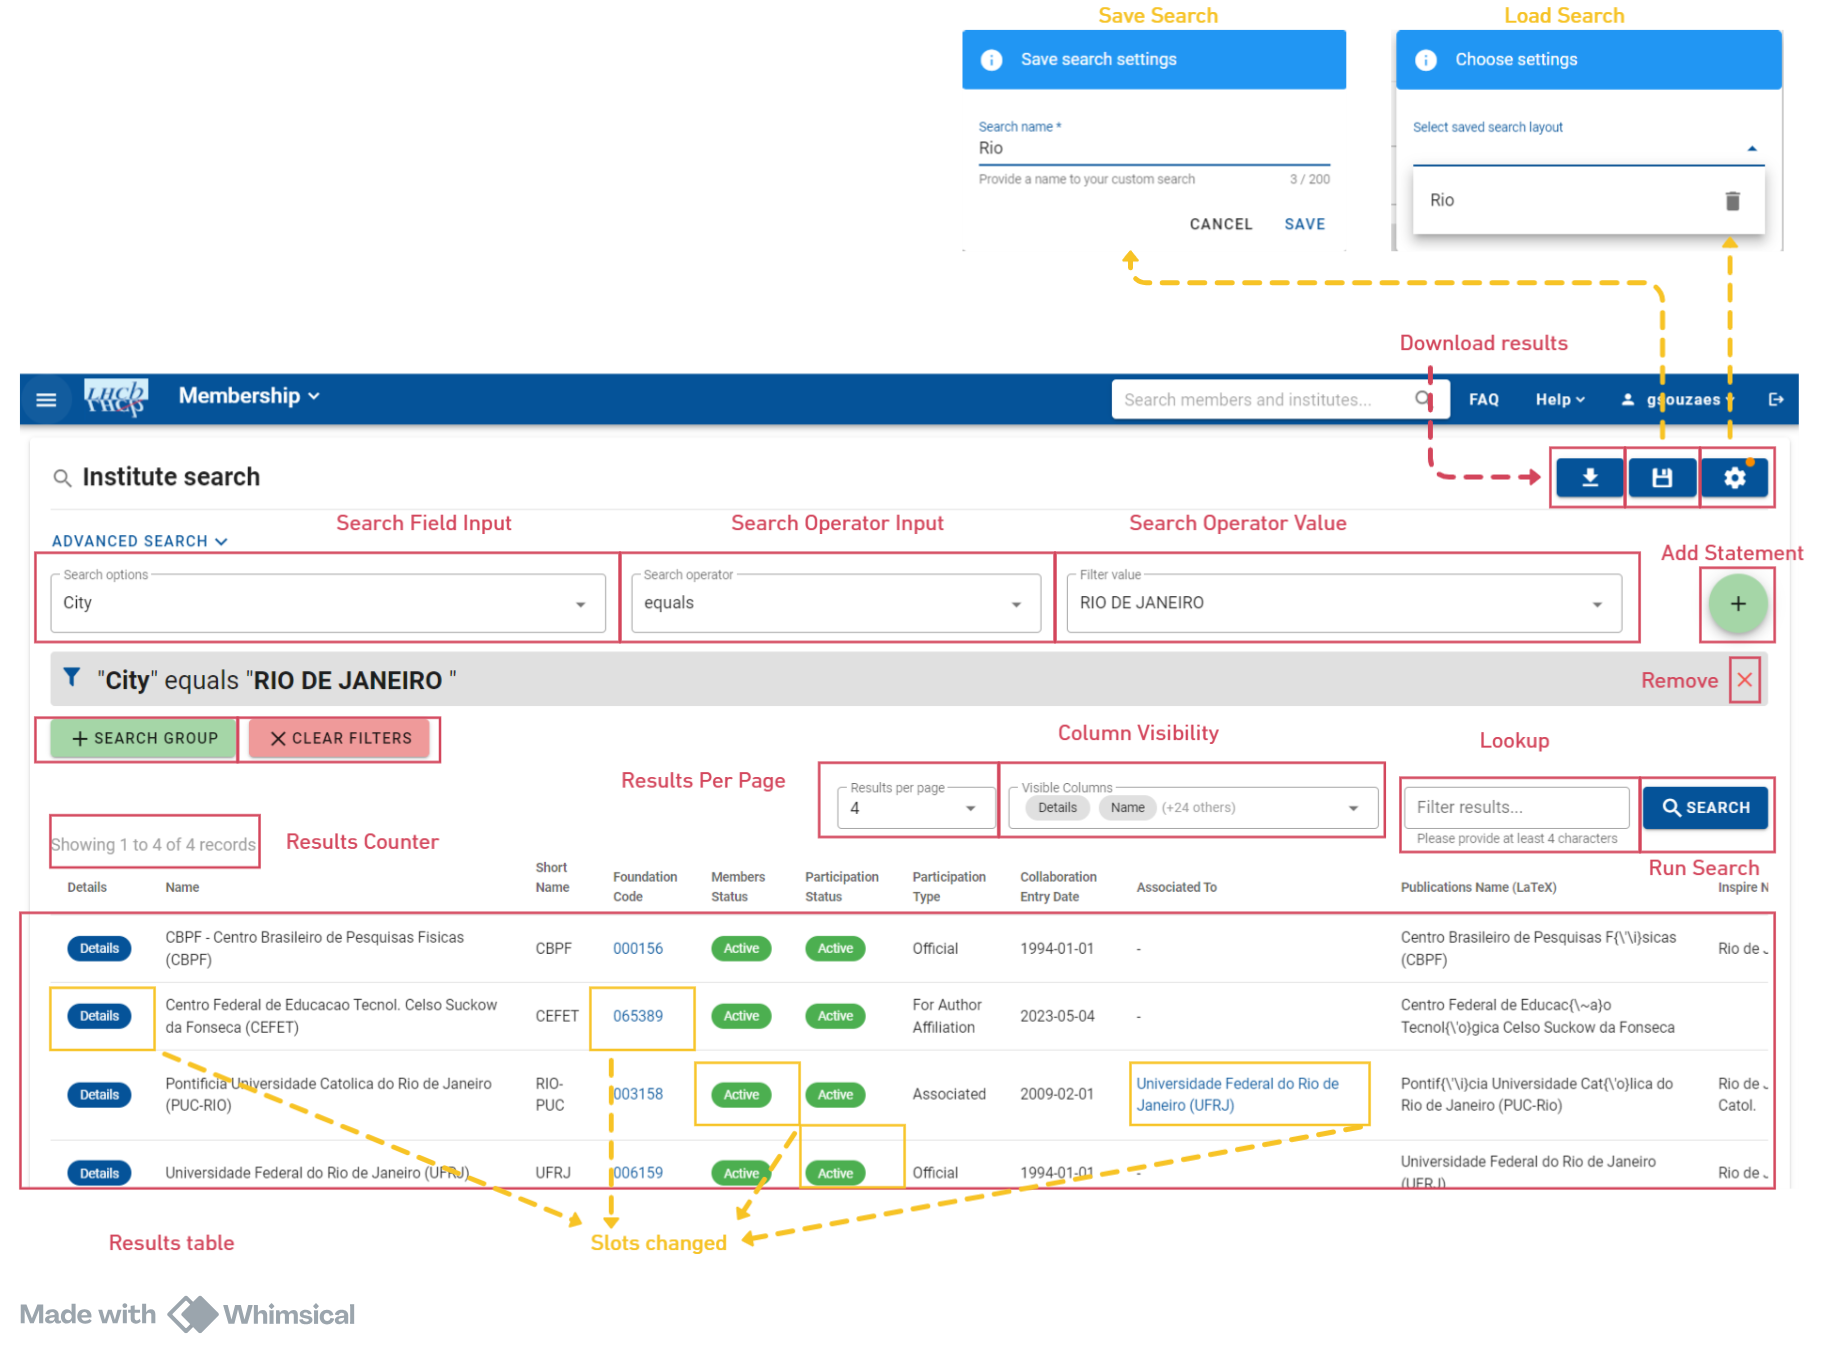
\includegraphics[width=1.0\linewidth]{figuras/search_components_marked.png}
    \caption{Institute Search Components.}
    \label{fig:search_components}
\end{figure}

\begin{figure} [H]
    \centering
    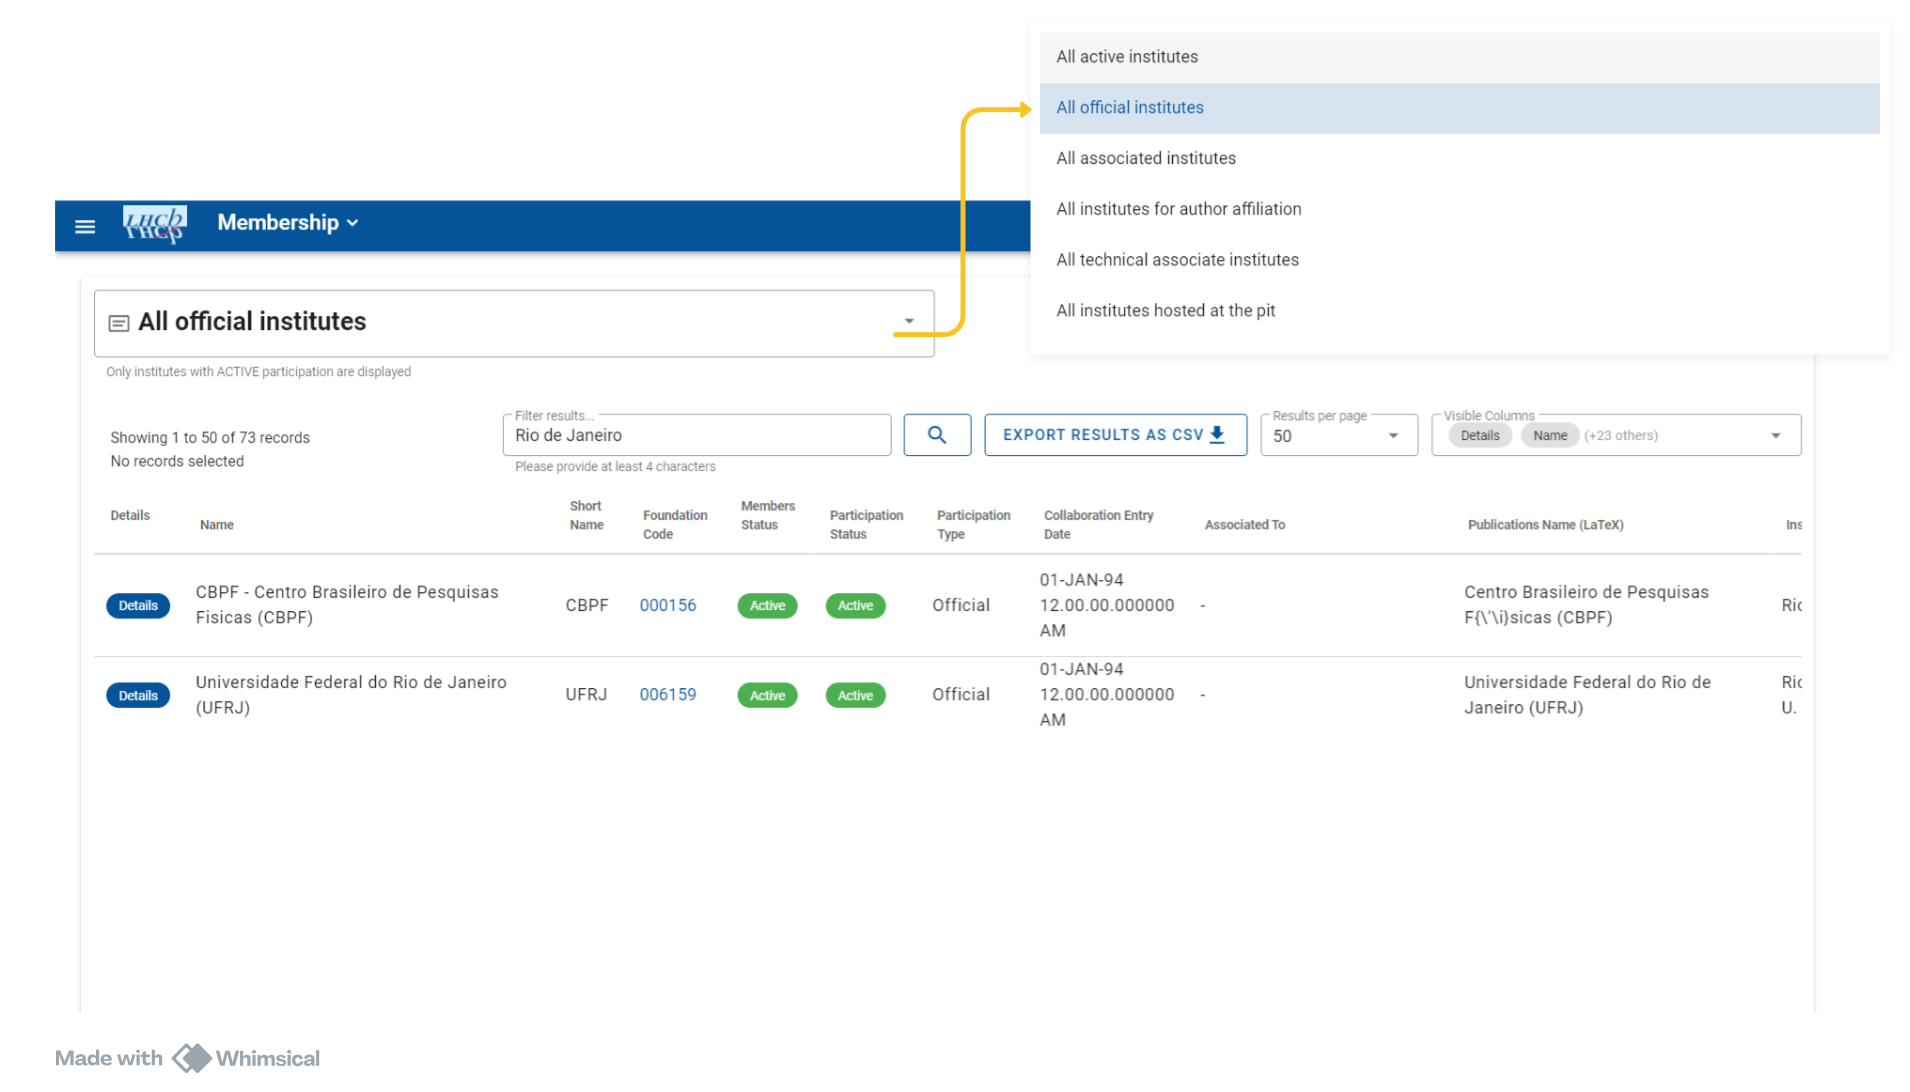
\includegraphics[width=1\linewidth]{figuras/simple_search.png}
    \caption{Simpler search visualization to list all Institutes according to their Participation Type.}
    \label{fig:simple_search}
\end{figure}

\section{Membership Implementation} 

\paragraph{} The implementation of the Membership system occurred within a period when the Hexagonal Architecture was firmly established as the chosen design paradigm for the Glance systems. Consequently, the Membership system does not exhibit a heterogeneous architectural approach similar to that of the Authorship system. The implementation provided the same existing functionalities and mostly improved use cases that benefit from the new Super Search and introduced approval workflows and interfaces with graphs.

\subsection{The Membership Architecture}

\paragraph{} It was established by the team that the Membership system would encompass the Authorship system and proceed to integrate the additional functionalities within the same application, as Authorship inherently falls within the purview of the Membership system's responsibilities. Unlike the singular context termed \verb|Authorship| within the Authorship system, the Membership system encompasses multiple requirements that do not uniformly align within a single domain. Here, the concept of Bounded Context (BC) as described on \cite{fowler2014bounded} significantly enhances the structural organization of the application. Bounded Context strategically addresses the complexities of large models and team coordination by partitioning a system into distinct segments, each characterized by its cohesive domain. This methodology not only facilitates a clearer segmentation of the system's components but also enhances team communication and understanding. Central to DDD is the creation of software that accurately reflects the domain's foundational models, fostering a shared language between developers and domain experts. This shared or Ubiquitous Language ensures consistency within a Bounded Context, while also acknowledging the impracticality of a singular model spanning a vast system. DDD advocates for the division of the system into Bounded Contexts, each with a model that maintains internal consistency yet may diverge from others, particularly concerning common concepts such as Members. An LHCb Member in the \verb|Member| context/namespace contains all the registration information the collaboration stores for its members, including the profile picture, list of Appointments, Employment, and more. A Member in the \verb|Authorship| context, on the other hand, is an Author and only contains the required information for authorship purposes. Communication between Bounded Contexts is done using the Classes from the Application Layer (Handlers and Repository Interfaces) which can have dependencies from Application-layer classes of a different BC. Inside the same BC, dependencies still point inwards (Infrastructure classes depend on Application-layer classes, which depend on Domain classes).


\paragraph{} The Modular Monolith concept is relatively recent in the Software Engineering literature. Ruoyu Su and Xiaozhou Li conducted a literature review on \cite{su2024modular} and defined a Modular Monolith as ``a software architecture pattern that strategically combines the simplicity of a monolithic structure with the advantages of microservices. In this approach, the system is organized into loosely coupled modules, each delineating well-defined boundaries and explicit dependencies on other modules." This definition is similar to the classical Monolith definition because it still envisages the application as a single deployable unit, ensuring simplicity in deployment and operation management (as it is not necessary to ensure compatibility of different service versions such as in microservices). However, it differs in that it emphasizes modularity, loose coupling, and independence within the application's internal structure, promoting ease of development, testing, and potential for scaling specific parts of the application without the need to scale everything. Loose coupling is achieved by defining clear dependencies between the modules through interface contracts. Another major difference between the classical monolithic application and a Modular Monolith is that the latter tends to incentivize code organization based on different Domains instead of class type (Controller, Model, Repository, etc.) as described in Shopify's engineering article \cite{ShopifyModularMonoly}. In the Membership context, each Bounded Context can be seen as an independent module, with its own domain definitions and the dependencies between modules modules occur through the Application layer in module's use cases are exposed. Figure \ref{fig:membership_bc} illustrates the Membership as a Modular Monolith. Each module has its own namespace in the application.

%\paragraph{} As described in Shopify's engineering article \cite{ShopifyModularMonoly}, a modular monolith architecture involves structuring a single codebase into well-defined, independent modules. Each module represents a specific business domain or functionality but is part of the same application and deployment unit. This approach maintains the simplicity of deployment and operational characteristics of a monolith while encapsulating business logic within clear boundaries, similar to microservices. Modular monoliths aim to balance the rapid development and deployment benefits of a monolithic architecture with the flexibility and scalability often associated with microservices. By defining strict boundaries around modules, a modular monolith can prevent the common pitfalls of traditional monolithic applications, such as tight coupling and complexity, making the system more maintainable and scalable within the confines of a single codebase. By introducing Bounded Contexts and decoupling the frontend and backend code, the Membership system was developed as a Modular Monolith. Figure \ref{fig:membership_bc} represents visually some of the Membership BCs.

\begin{figure}[H]
    \centering
    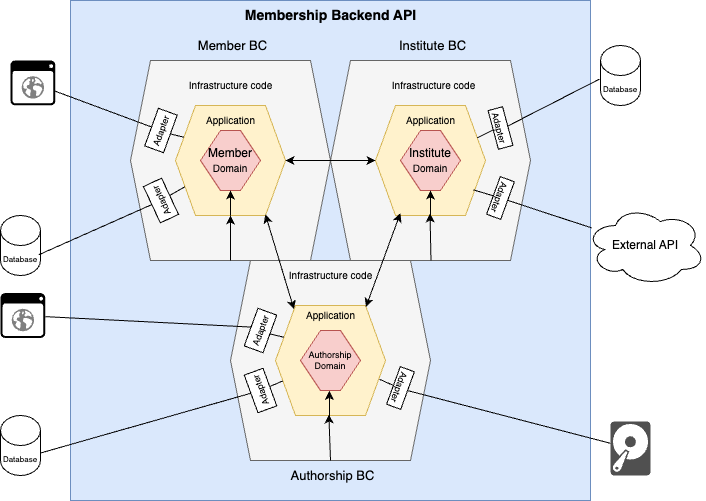
\includegraphics[width=1\linewidth]{figuras/modular_monolith (7).png}
    \caption{Membership Bounded Contexts.}
    \label{fig:membership_bc}
\end{figure}


\subsection{Workflow Tracking}

\paragraph{}Membership Version 2 introduced significant enhancements, notably in the tooling for managing internal processes via an approval workflow. The primary motivation for these developments was the newcomer registration process, as detailed in section \ref{subsec:workflow_project_cap_2}. After conducting a series of interviews with the Secretariat, the process was remodeled, as depicted in Figure \ref{fig:newcomer_wf_refactor}. A key modification is the implementation of a cron job that continually queries CERN's HR internal APIs. This automation detects newcomer registrations at CERN and initiates the LHCb registration process by creating a \verb|NewcomerRegistrationRequest|. This temporary entity encapsulates all information from CERN HR, along with additional details necessary for LHCb registration, and links to the \verb|NewcomerRequestState| entity that tracks the request's current status. The newly introduced workflow has a similar number of actions when compared to the one shown in section \ref{subsec:workflow_project_cap_2}, but its key innovation lies in automating information transfer, thereby reducing manual work. Also, by creating a multi-step approval process, it also reduces the number of incorrect information persisted in the database. In the most common scenario, newcomers submit all required information to CERN HR and provide additional details for LHCb. Assuming the accuracy of this information, the Team Leader approves the request with a simple button press, a procedure also followed by the Secretariat as exemplified in Figure \ref{fig:wf_management_page}. Notifications are automatically dispatched by the system in response to state changes, significantly reducing the volume of emails exchanged among participants. Following the implementation of the newcomer registration workflow, the use of the LHCb PDF registration form was discontinued. Each state change in the approval process required a Handler class (linked to an API endpoint called by an action button in the interface) to update the \verb|NewcomerRequestState| in response to an event (exemplified in listing \ref{lst:handle_wf}). In other words, there was no state transition function to automatically evolve the state based on an event publication. This aspect improves when workflows are modeled as automatons.

\begin{figure}[H]
    \centering
    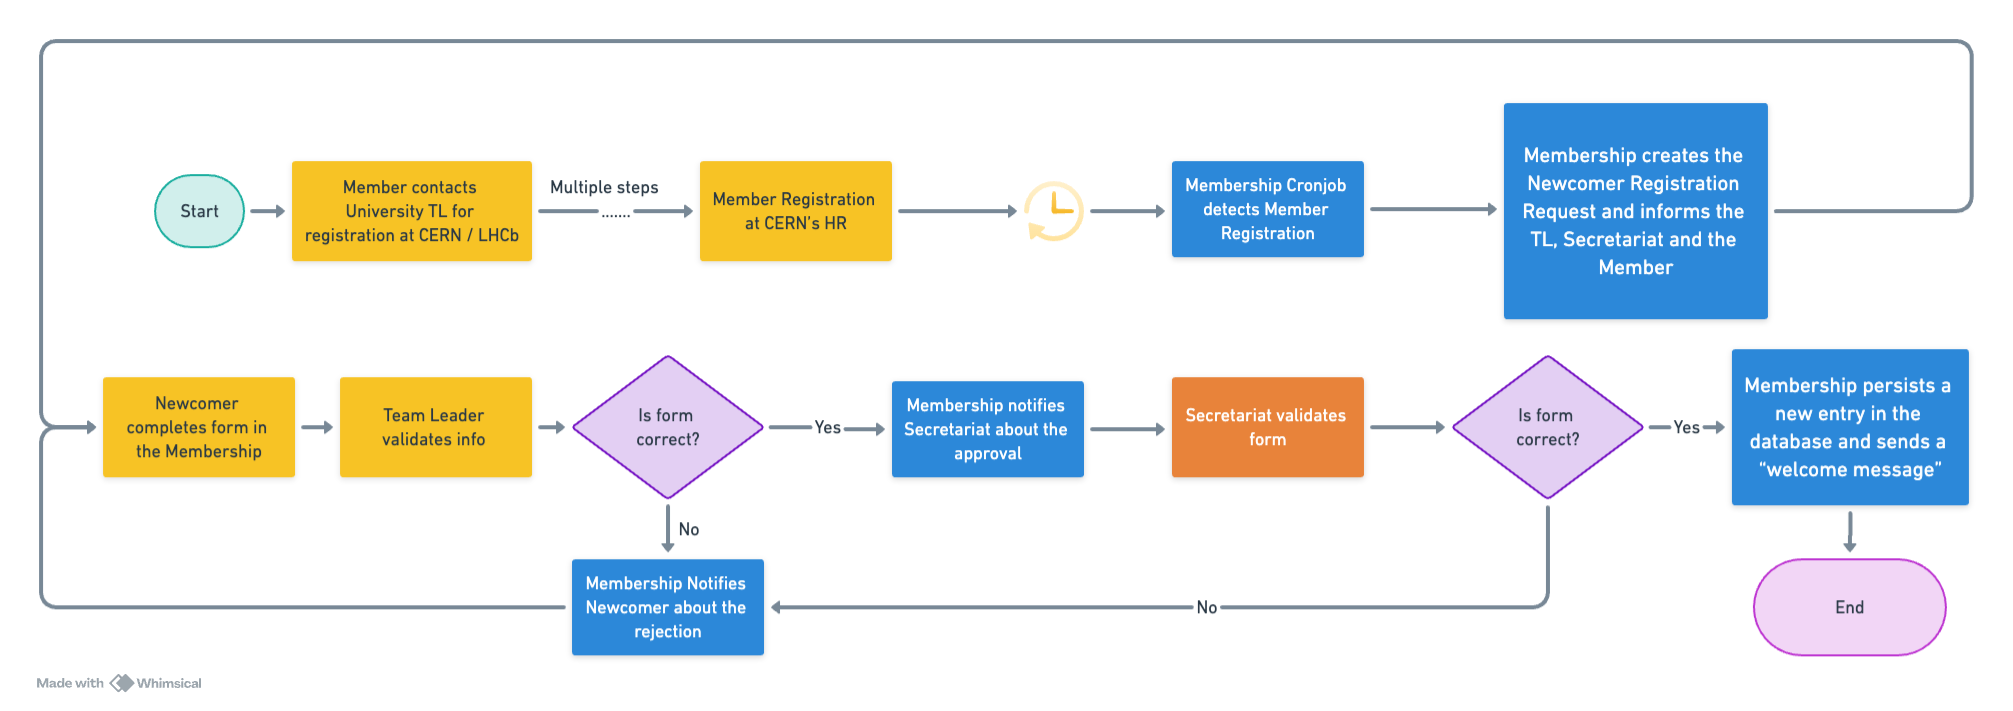
\includegraphics[width=1\linewidth]{figuras/newcomer_wf_refactor_2.png}
    \caption{Newcomer registration workflow refactored.}
    \label{fig:newcomer_wf_refactor}
\end{figure}

\begin{figure}[H]
    \centering
    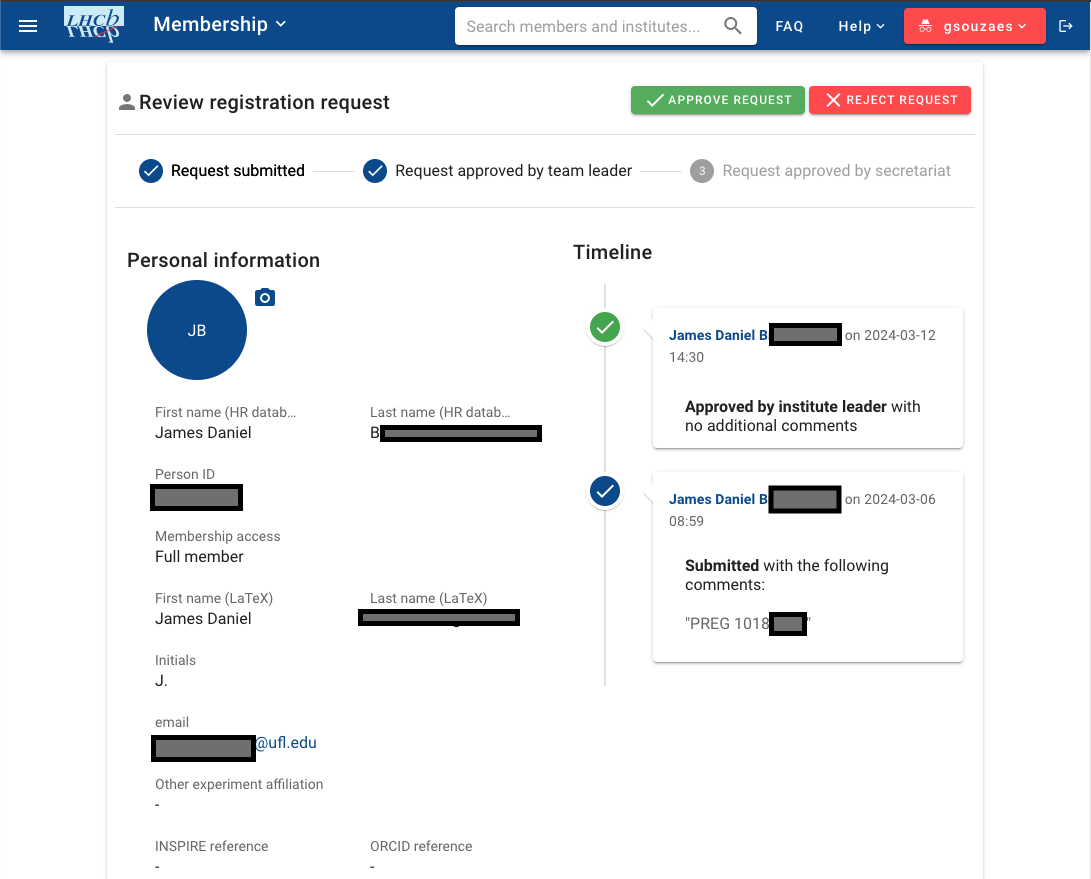
\includegraphics[width=0.65\linewidth]{figuras/wf_management_page.png}
    \caption{Newcomer Request management page pending Secretariat approval.}
    \label{fig:wf_management_page}
\end{figure}

\paragraph{} The release of the Newcomer registration workflow catalyzed the development of additional multi-step approval workflows for Members transitioning to different Institutes, altering Professions, or extending their Employments. Similar to the Newcomer registration process, these workflows were developed with a Command and Handler for each state transition (such as a button pressed on the interface to change a request to ``Rejected"), leading to a phenomenon known as class explosion. This term describes a situation where the number of classes in a system becomes excessively large as a result of attempts to accommodate every possible variation of a problem or requirement through inheritance or the creation of fine-grained classes for every piece of functionality. It was observed that the approval and rejection operations predominantly involved updating the state of the \verb|Request| entity (the possible states are shown in a state transition diagram in Figure \ref{fig:states}), as exemplified in listing \ref{lst:handle_wf}. The way to avoid these unnecessary Handlers is to model the approval workflows as automatons and introduce a state transition function that could be called from a single Handler based on events published by other parts of the system. In practice, this would mean that instead of having one API endpoint for each action button (buttons to approve a request, reject a request, and submit a request) there could be one generic endpoint to post events mapped to a Handler that calls the state transition function passing the event as argument.

\paragraph{} The diagram from Figure \ref{fig:states} can be formalized using the automaton concept already explored. Let $ G=\left(X, \Sigma, f, \Gamma, x_0, X_m\right)$ be the automaton describing the approval process. Then 
$$
X=\{U, V, W, X, Y, Z\}; \Sigma=\{a, b, c, d, e, f, g, h\}
$$
For any state $x \in X$ and event $\sigma \in \Sigma$ :
$$
f(x, \sigma)= \begin{cases}V & \text { if }(x, \sigma)=(U, a) \\ T & \text { if }(x, \sigma)=(U, b) \\ W & \text { if }(x, \sigma)=(V, d) \\ T & \text { if }(x, \sigma)=(V, e) \\ V & \text { if }(x, \sigma)=(W, c) \\ T & \text { if }(x, \sigma)=(W, h) \\ Y & \text { if }(x, \sigma)=(T, f) \\ Z & \text { if }(x, \sigma)=(T, g) \\ T & \text { if }(x, \sigma)=(Y, h) \\ V & \text { if }(x, \sigma)=(Y, c) \\ x & \text { otherwise }\end{cases}
$$
$$
\Gamma(K)=\Sigma \text { for all } K \in X; x_0=U; X_m=\{Z\}
$$

\paragraph{} The same formulation applies to all the different Membership approval workflows currently available involving the Secretariat and Team Leaders. 

\paragraph{} Concurrently with the necessity to reduce the class explosion (evident by the number of classes in the directory structure in \ref{dirTree}) and the implementation of a new system for managing LHCb publication approvals, a pressing need emerged for an enhanced workflow tracking solution. This solution should effectively manage a complex graph scenario where the user specifies \textbf{two states and a sequence of events required for transitioning between these states}. The existing challenge is that previously demonstrated graphs (such as in Figure \ref{fig:states}) typically feature a single event linking two states. The proposed solution, therefore, must accommodate more intricate interactions handling multiple events within state transitions.

\begin{lstlisting}[language=php, caption={Example of handle method to deal with the press of the approve button by the TL (Team Leader).}, basicstyle=\tiny, label=lst:handle_wf]
public function handle(ApproveNewEmploymentRequestCommand $command): int
    {
        $newEmploymentRequest = $this->workflowReadRepository
            ->findNewEmploymentRequest($command->memberId());
        $instituteLeadersIds = $this->workflowReadRepository->findInstituteLeaderIds($newEmploymentRequest->instituteId());

        $newEmploymentRequest->addState(
            new WorkflowState(
                $this->workflowRepository->findNextNewEmploymentRequestStateId(),
                WorkflowState::APPROVED_BY_INSTITUTE_LEADER,
                $command->comments(),
                $command->agentId()
            ),
            $command->memberId(),
            $instituteLeadersIds
        );

        $this->workflowRepository->insertStates($newEmploymentRequest, $command->agentId());
        $this->eventDispatcher->dispatchAll($newEmploymentRequest->releaseEvents());
        return $newEmploymentRequest->id();
    }
}
\end{lstlisting}


\noindent % Prevent indentation at the beginning of the environment
\begin{minipage}{.55\linewidth}
\label{dirTree}
\dirtree{% Your directory tree structure
.1 Application.
.2 ApproveChangeInstituteRequest.
.2 ApproveChangeProfessionRequest.
.2 ApproveNewEmploymentRequest.
.2 ApproveNewcomerRequest.
.2 .....
.2 GetChangeInstituteRequestDetails.
.2 GetChangeProfessionRequestDetails.
.2 .....
.2 GetNewEmploymentRequestDetails.
.2 GetNewcomerRequestDetails.
.2 ....
.2 RejectChangeInstituteRequest.
.2 RejectChangeProfessionRequest.
.2 RejectNewEmploymentRequest.
.2 RejectNewcomerRequest.
.2 SubmitChangeInstituteRequest.
.2 SubmitChangeProfessionRequest.
.2 SubmitNewEmploymentRequest.
.2 SubmitNewcomerRequest.
}
\end{minipage}%
\hfill
\begin{minipage}{.5\linewidth}
\begin{figure}[H]
    \centering
    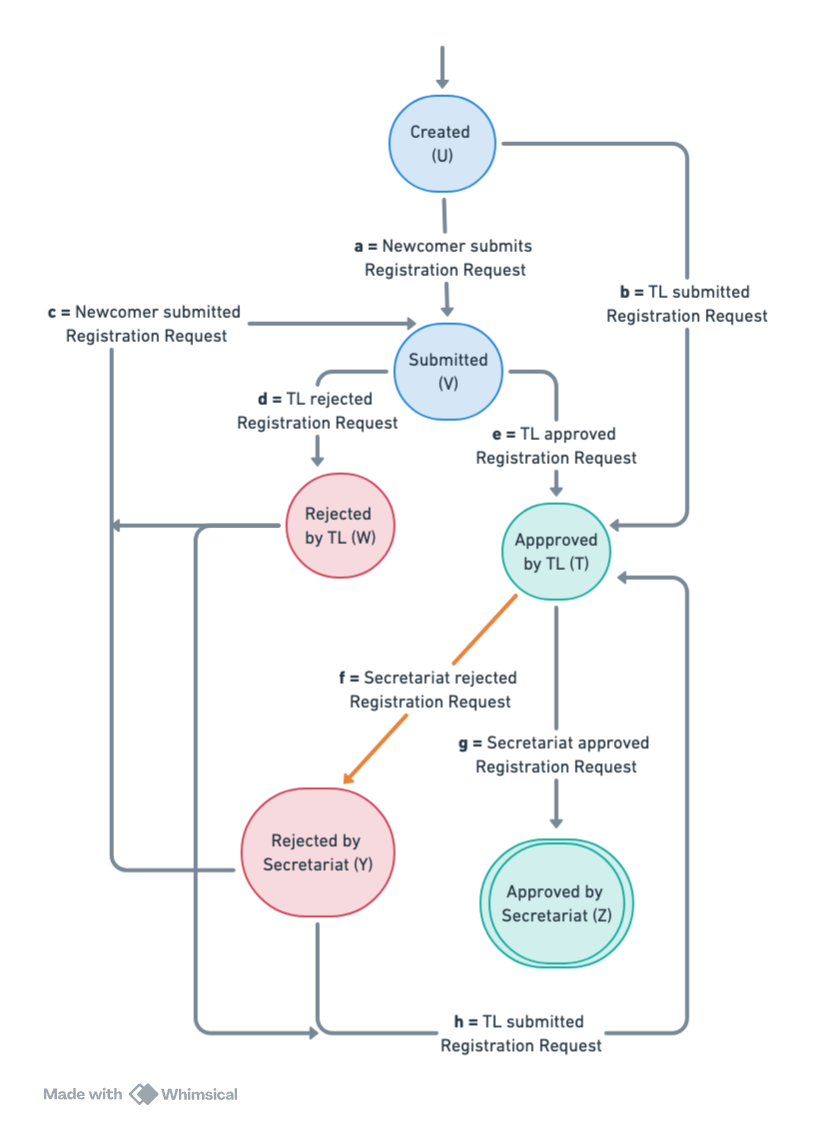
\includegraphics[width=1\linewidth]{figuras/approval_graph.png}
    \caption{Newcomer registration request graph.}
    \label{fig:states}
\end{figure}
\end{minipage}



\paragraph{} To address class explosion and minimize boilerplate code in state transitions, a new generic Workflow BC was developed. This was also inspired by the LHCb Analysis Lifecycle Management System (ALCM), which is designed around the concept of using graph theory to track the evolution and state transitions of various types of documents published by LHCb through their review procedures. The requirement for multiple events between transitions comes from ALCM, where a document usually goes to the next stage in the review process based on multiple approvals (events).

\paragraph{} In this scenario, the review stage/status is not represented as a state in a directed graph because changes are controlled by a \textbf{list} of specific events. To address this, a generic Workflow engine is introduced to manage the lifecycle of an entity. The process begins with the creation of a new Workflow class, which accepts an array of Transitions in its constructor. Each Transition consists of an initial State, a target State, an array of Events that occur in relation to the tracked entity, and an array of Conditions (analogous to events) required for a State change from the current to the target. Figure \ref{fig:abc_graph} exemplifies the registration of a Workflow with 3 States ($A$, $B$ and $C$). The instantiation of a new Workflow class is done is listing \ref{lst:figure_wf}. Transitioning from $A$ to $B$ requires the events $x$, $y$ and $z$. From $B$ to $C$ only $m$ and $n$. The automaton that describes this Workflow is $ G=(X, \Sigma, f, \Gamma, x_0, X_m)$ where
$$
X=\{A, A_1, A_2, A_3, A_4, A_5, A_6, B, B_1, B_2, C\}; \Sigma=\{x, y, z, m, n\}
$$

\noindent
Let $n_{i j}$ be the number of Conditions between State $i$ and State $j$. The number of intermediate states for each pair $(i, j)$ is $2^{n_{i j}}-2$. This indicates that the number of intermediate states grows exponentially with the number of events, emphasizing the need to register states only on demand, as demonstrated in the \verb|handleNewEvent| method in listing \ref{lst:InnerStatesGraph}.


\paragraph{} For this reason, this Workflow engine is designed in a way that intermediate states are abstracted from the user and handled internally, being only necessary to provide the initial and final States (the Stages). In the present work, a State registered by the user is also referred to as a Stage, these are the meaningful States to the final application user which must be displayed on the interface. When registering a new Workflow, the marked State will always be the current Stage in Transition without target Stage. The class shown in listing \ref{lst:InnerStatesGraph} does the processes of evolving the intermediate states and is used by the Transition class \verb|isFulfilled| method, shown in listing \ref{lst:isFulfilled}, to determine if all the Transition Conditions were satisfied. 

\paragraph{} This approach allows for the registration of all relevant \verb|State|s and \verb|Transition|s through which an Entity can progress, as exemplified in listing \ref{lst:figure_wf}.

\begin{figure} [H]
    \centering
    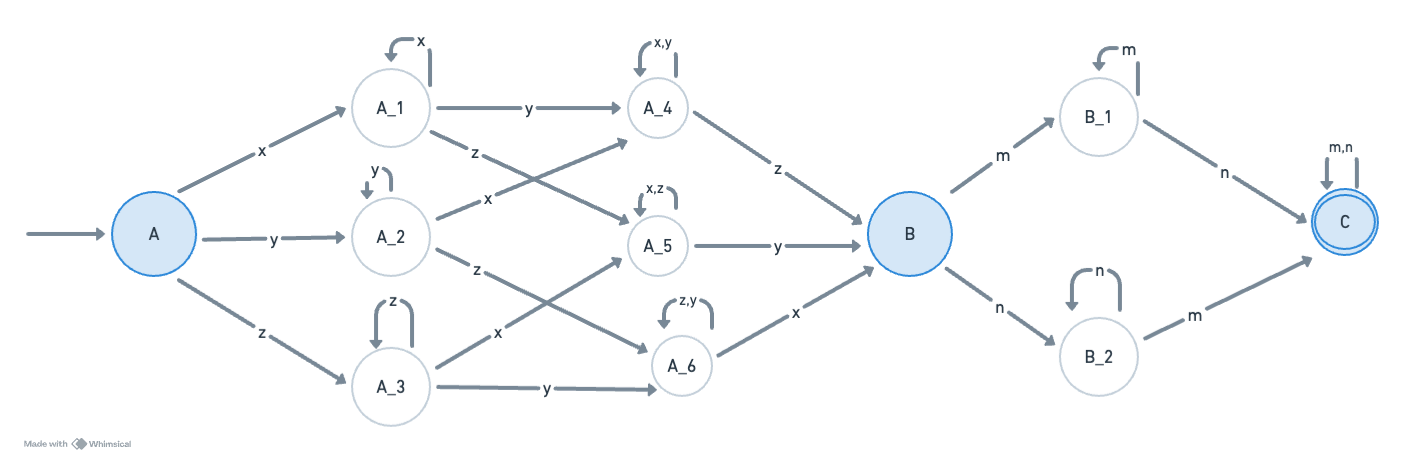
\includegraphics[width=1\linewidth]{figuras/abc_graph.png}
    \caption{Graph for three Stages $A$, $B$, and $C$. To go from $A$ to $B$, events $x$, $y$, and $z$ must occur. To go from $B$ to $C$, events $m$ and $n$ must occur. $A$, $B$, and $C$ are provided by the user and the remaining States are dynamically generated.}
    \label{fig:abc_graph}
\end{figure}

\begin{lstlisting}[language=php, caption={Workflow registration for a Figure document to be approved by the EB.}, basicstyle=\tiny, label=lst:figure_wf]
$workflow = new Workflow(
            $event->entityId(),
            FigureStage::DRAFTING,
            [
                new Transition(
                    FigureStage::DRAFTING, //current stage //A
                    FigureStage::TO_BE_REVIEWED, //next stage //B
                    [Condition::create(FigureReadyForReview::ACTION_ID, null)], //analogous to x, y, z
                    [],
                ),
                ...
                new Transition(
                    FigureStage::TO_BE_REVIEWED, // B
                    FigureStage::APPROVED, // C
                    [Condition::create(FigureApproved::ACTION_ID, null)], //analogous to m,n
                    [],
                ),
                new Transition(FigureStage::APPROVED, null, [], [],),
            ]
        );
        $this->repository->registerWorkflow($workflow, $event->agentId());
\end{lstlisting}


\begin{lstlisting}[language=php, caption={Class that handles intermediate states.}, basicstyle=\tiny, label=lst:InnerStatesGraph]
class InnerStatesGraph {
    private $states = [];
    private $events = [];
    private string $currentState;
    private string $finalState;

    public function __construct(string $initialStateName, string $finalStateName) {
        $this->currentState = $initialStateName;
        $this->finalState = $finalStateName;
        $this->states[$initialStateName] = [];
    }

    public static function fromTransition(Transition $transition): self {
        $graph = new self($transition->currentStageId(), $transition->targetStageId());
        foreach ($transition->entryConditions() as $condition) {
            $graph->addEvent($condition->actionId() . "-" . $condition->memberId());
        }
        return $graph;
    }

    public function addEvent(string $eventKey): void {
        $this->events[$eventKey] = $eventKey;
    }

    public function handleNewEvent(ActionPerformed $action): void {
        $eventKey = $action->actionId();
        if (!in_array($eventKey, $this->events)) {
            $eventKey = $eventKey . "-" . $action->agentId();
        }
        if (!in_array($eventKey, $this->events)) {
            return;
        }
        if ($this->currentState === $this->finalState) {
            return;
        }
        $currentEvents = $this->states[$this->currentState] ?? [];
        
        if (!in_array($eventKey, $currentEvents)) {
            $currentEvents[] = $eventKey;
            sort($currentEvents);
            $newStateName = implode(",", $currentEvents);
            $this->states[$newStateName] = $currentEvents;
            $this->currentState = $newStateName;
        }

        if ($this->isFinal($currentEvents)) {
            $this->currentState = $this->finalState;
        }
    }
    private function isFinal($eventsReceived): bool {
        return count($eventsReceived) === count($this->events);
    }
    public function getCurrentState() {
        return $this->currentState;
    }
\end{lstlisting}

\begin{lstlisting}[language=php, caption={Transition class isFulfilled method.}, basicstyle=\tiny, label=lst:isFulfilled]
public function isFulfilled(): bool
    {
        $graph = InnerStatesGraph::fromTransition($this);
        foreach ($this->performedActions as $action) {
            $graph->handleNewEvent($action);
        }
        return $graph->getCurrentState() == $this->targetStageId;
    }
\end{lstlisting}


%todo: talk about using the theory to validate automaton registration
%todo maybe display the code 

\paragraph{} The Workflow class implements a check to prevent the registration of lifecycles with locks. This means that if $G$ is an automaton that describes the entity lifecycle, then $\overline{L_m(G)}=L(G)$, otherwise there are locks. To perform this validation, it is not necessary to analyze any intermediate states, as those are internally handled by the system in a way that locks will not arise. To exemplify this validation, a higher-level view of the graph from Figure \ref{fig:abc_graph} is displayed in Figure \ref{fig:abc_graph_simple}. In this case the automaton $ G=(X, \Sigma, f, \Gamma, x_0, X_m)$ with
$$
X=\{A, B, C\}; \Sigma=\{v, k\}
$$
\noindent
In the given example, a visual inspection suffices to ascertain that the automaton exhibits nonblocking behavior. The \verb|HighLevelStatesGraph| class, referenced in listing \ref{lst:HighLevelStatesGraph}, computationally confirms this by identifying all viable paths originating from the initial State. The class checks the \text{no-lock condition:} \(\overline{L_m(G)}=L(G)\) by executing the following steps: First, it uses the method \verb|findAllPaths($startState)| to generate all possible paths from the initial State, which represent the generated language \(L(G)\). It then filters these paths using \verb|filterPathsEndingAtFinalState($paths)| to retain only those paths that lead to the final (marked) State, representing the marked language \(L_m(G)\). Next, the class verifies whether every path in the generated language \(L(G)\) can reach the marked State. This is done in the \verb|isNonblocking()| method, which checks if all paths found in \(L(G)\) are also present in the filtered paths leading to the final State. If there exists any path in \(L(G)\) that cannot be extended to reach the marked State, the method returns \verb|false|, indicating that \(\overline{L_m(G)} \neq L(G)\), and thus, there are locks in the system. If all paths can reach the marked State, the method returns \verb|true|, confirming \(\overline{L_m(G)} = L(G)\) and indicating a nonblocking system.



\paragraph{} This class functionality is used in the Workflow class constructor, which leverages it to validate the sequence of transitions. If a transition sequence is detected that does not comply with the nonblocking condition, the constructor raises an exception, thereby preventing the creation of a workflow that could potentially lead to a deadlock or an incomplete process execution.

\begin{figure} [H]
    \centering
    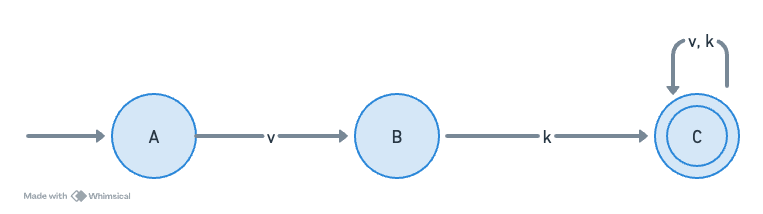
\includegraphics[width=1\linewidth]{figuras/abc_graph_simple.png}
    \caption{Graph for three Stages $A$, $B$, and $C$.}
    \label{fig:abc_graph_simple}
\end{figure}

\paragraph{} The Workflow BC provides a \verb|SaveAction| subscriber that can be invoked whenever an Event occurs to advance the State in the Entity workflow graph. \textbf{This subscriber acts as the State transition function of the system, updating the State according to an Event received.} The lifecycle will evolve through the intermediate States until all Conditions are met and a Transition from a State to a Stage occurs, indicating that the Entity State has moved to the next Stage (target State registered by the user). Through the \verb|SaveAction| subscriber, the application backend is equipped with a singular Application Use Case to post a generic Event.

\paragraph{} For Membership, this means that instead of having a unique Handler/Command pair for changing the entity State (as illustrated in listing \ref{lst:handle_wf}), a generic \verb|PostEventHandler| could be utilized for all approvals and rejections, solving the class explosion problem. This Handler would emit an Event that is captured by the \verb|SaveAction| invokable class (shown in listing \ref{lst:saveAction}). If a Transition is fulfilled (such as when the Secretariat rejects a Newcomer Request, moving it from the State \textbf{``Approved by TL"} to \textbf{``Rejected by Secretariat"} as the \textbf{``Secretariat Rejects Request"} Condition in the Transition from \textbf{``Approved by TL"} to \textbf{``Rejected by Secretariat"} is satisfied by the \textbf{``Secretariat Rejected Request"} Event. This Transaction is marked in orange in Figure \ref{fig:states}) a new Transition Fulfilled Event is dispatched. This can be monitored to, for instance, trigger a notification.

\begin{lstlisting}[language=php, caption={Workflow registration for a Figure document to be approved by the EB.}, basicstyle=\tiny, label=lst:saveAction]
final class SaveAction
{
    private $repository;
    private $eventDispatcher;
    ...
    public function __invoke(ActionPerformed $event): void
    {
        $workflow = $this->repository->findWorkflow($event->entityId());
        $workflow->recordPerformedAction($event);
        $this->repository->savePerformedAction(
            $event->entityId(),
            $event->actionId(),
            $event->agentId(),
            $event->comments()
        );

        if ($workflow->currentTransitionFulfilled()) {
            $workflow->proceed();
            $this->repository->updateWorkflowStage(
                $workflow->entityId(),
                $workflow->currentStageId(),
                $event->agentId()
            );
        }
        $this->eventDispatcher->dispatchAll($workflow->releaseEvents());
    }
}
\end{lstlisting}

\begin{lstlisting}[language=php, caption={Class to prevent blocking states.}, basicstyle=\tiny, label=lst:HighLevelStatesGraph]
class HighLevelStatesGraph {
    private $transitions = [];
    private $states = [];
    private $initialState;
    private $finalState;

    public static function fromTransitions(array $transitions, $initialState): self {
        $graph = new self($initialState);
        foreach ($transitions as $t) {
            $graph->addTransition($t->currentStageId(), $t->targetStageId());
        }
        return $graph;
    }

    public function __construct($initialState) {
        $this->initialState = $initialState;
    }

    public function addTransition($from, $to): void {
        $this->states[$from] = true;
        if ($to === null) {
            $this->finalState = $from;
        } else {
            $this->transitions[$from][] = $to;
            $this->states[$to] = true;
        }
    }

    public function isNonblocking(): bool {
        $allPaths = $this->findAllPaths($this->initialState);
        $pathsToFinal = $this->filterPathsEndingAtFinalState($allPaths);
        foreach ($allPaths as $path) {
            if (!in_array($path, $pathsToFinal)) {
                return false;
            }
        }
        return true;
    }

    public function isLocked(): bool {
        return !$this->isNonblocking();
    }

    private function findAllPaths($startState): array {
        $allPaths = [];
        $this->explorePaths($startState, [], $allPaths);
        return $allPaths;
    }

    private function explorePaths($current, $visited, &$paths, $path = ''): void {
        if (isset($visited[$current])) {
            return;
        }
        $visited[$current] = true;
        $path .= $path ? "->" . $current : $current;

        if (empty($this->transitions[$current])) {
            $paths[] = $path;
        } else {
            foreach ($this->transitions[$current] as $next) {
                $this->explorePaths($next, $visited, $paths, $path);
            }
        }
        $visited[$current] = false;
    }

    private function filterPathsEndingAtFinalState($paths): array {
        return array_filter($paths, function($path) {
            return strpos($path, $this->finalState) !== false;
        });
    }
}
\end{lstlisting}


\subsection{Features}
\paragraph{}The Membership system primarily manages the core data entities through profile pages. On a Member's profile page, LHCb Members, the Secretariat, and Team Leaders have the capability to view and update personal information. This includes changes to their publication name, profile picture, and initiating modifications to their Employment details such as Profession, Employment period, or Institute affiliation. Additionally, the system supports various other updates pertinent to a member's profile. Figure \ref{fig:member_profile} illustrates a Member's profile within the system.

\begin{figure} [H]
    \centering
    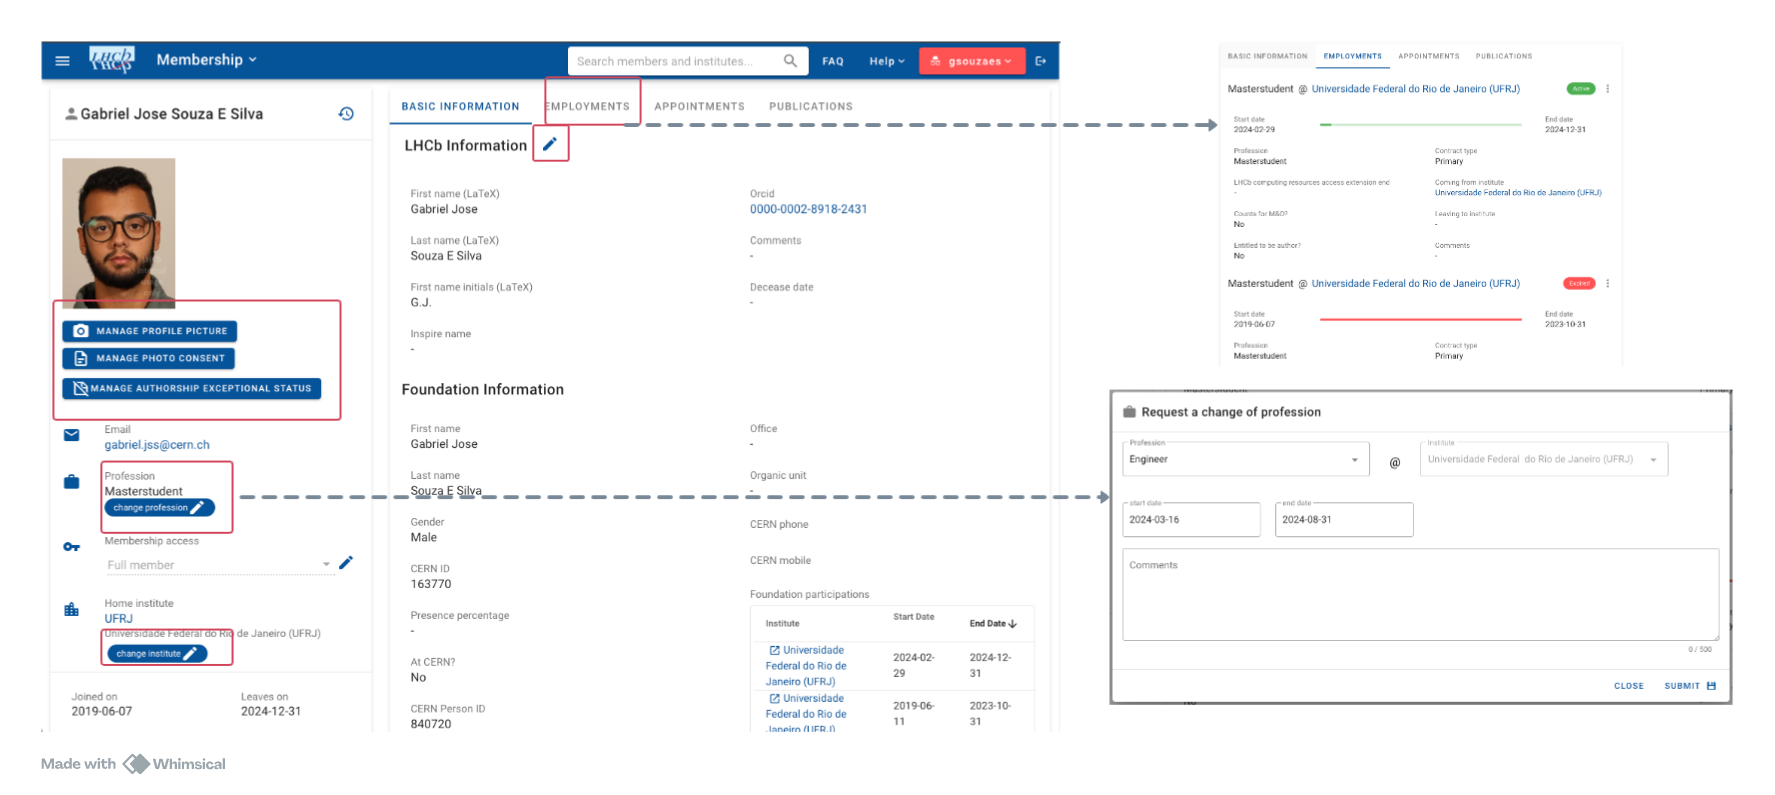
\includegraphics[width=1\linewidth]{figuras/profile.png}
    \caption{Membership Member profile.}
    \label{fig:member_profile}
\end{figure}

\paragraph{} The Institute profile page is primarily utilized by Team Leaders and Resource Coordinators for financial oversight, particularly regarding M\&O data. To facilitate access to M\&O information, an export feature is available, enabling the download of a CSV file that encapsulates the data presented on the interface. This functionality, among other user-centric enhancements, significantly augments the system's usability. Implementing such customizations within the Fence framework would be notably labor-intensive, as they extend beyond the basic capabilities of Fence's configuration files. Conversely, with Vue, developers have the flexibility to enrich components, for instance, by adding an export button using the Slots API. This adaptability also extends to the incorporation of complex data visualizations like the graphs visible in Figure \ref{fig:mb_institute_profile}, made feasible through the revamped architecture. Furthermore, the Institute profile page offers functionalities for editing an Institute's registration details and managing its Participations, with Figure \ref{fig:mb_institute_profile} illustrating the profile of the UFRJ Institute within the LHCb experiment.

\begin{figure} [H]
    \centering
    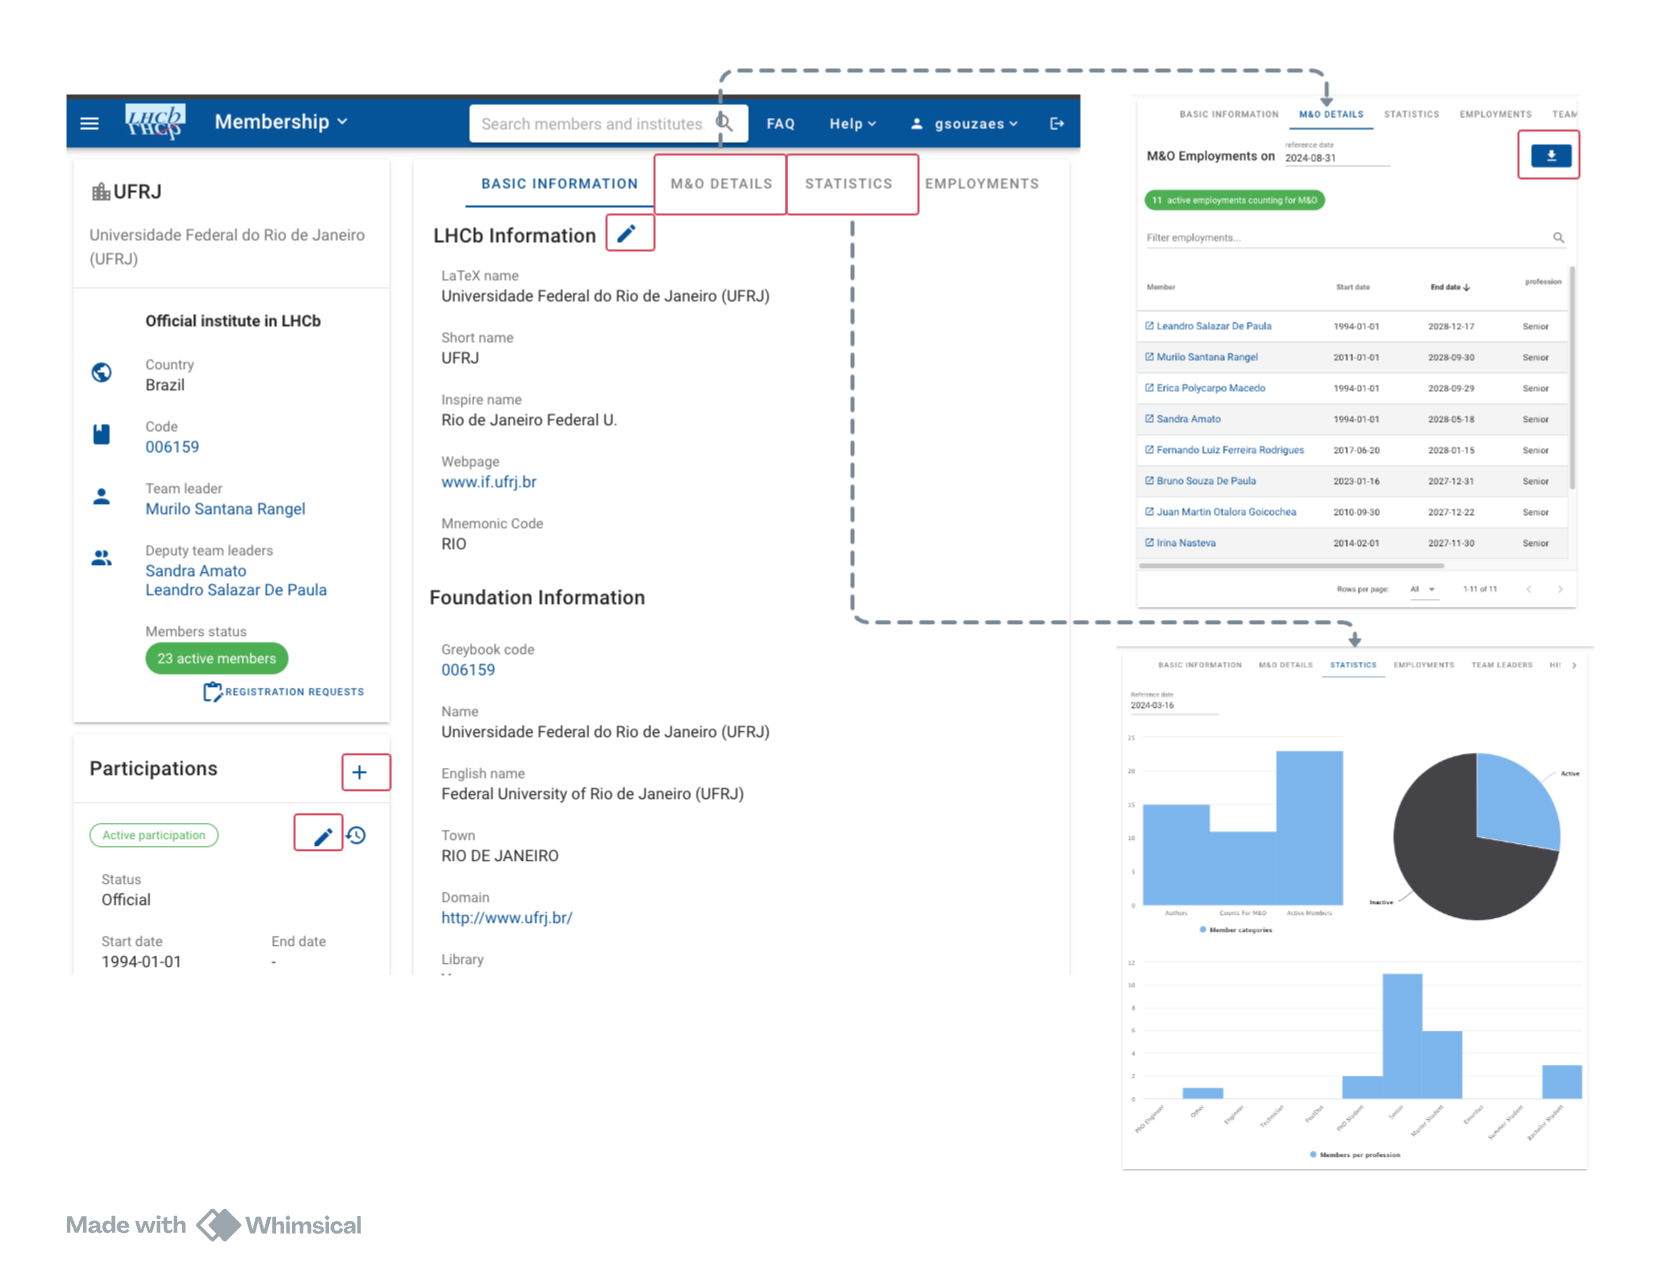
\includegraphics[width=1\linewidth]{figuras/mb_institute_profile.png}
    \caption{UFRJ Institute profile.}
    \label{fig:mb_institute_profile}
\end{figure}

\paragraph{} While Figure \ref{fig:wf_management_page} introduces the interfaces for workflow management, additional interfaces facilitate the management of all available workflows. Specifically, the management page for the Change Profession Workflow is shown in Figure \ref{fig:change_profession_wf}. Through this interface, Team Leaders and the Secretariat can review the list of all active processes. Analogous interfaces are available for managing the Change Institute Workflow, as well as the New Employment and Extend Employment Workflows, streamlining the oversight and administration of these processes.

\begin{figure} [H]
    \centering
    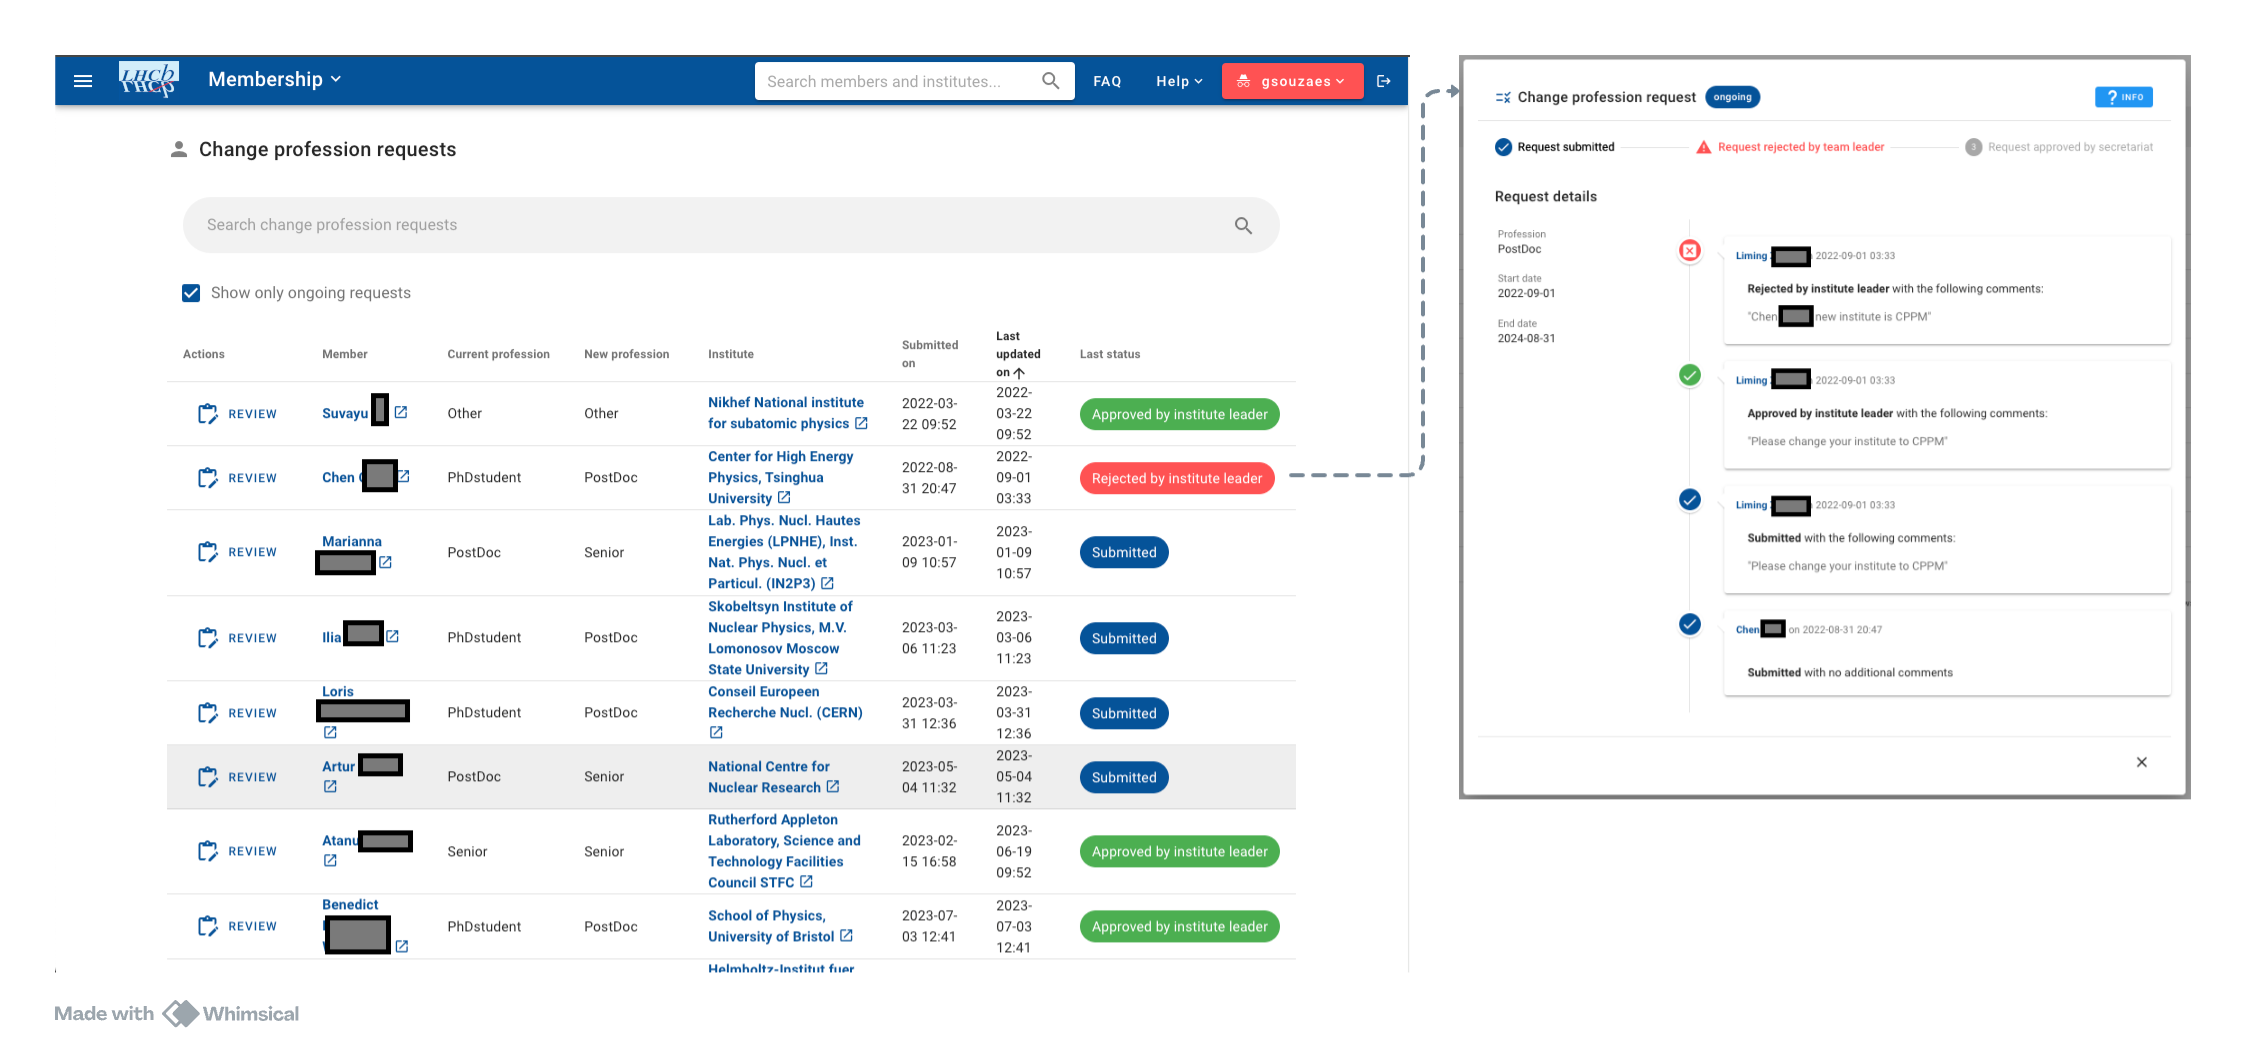
\includegraphics[width=1\linewidth]{figuras/change_profession_wf.png}
    \caption{Change Profession Request being reviewed.}
    \label{fig:change_profession_wf}
\end{figure}

\paragraph{} Graphs were introduced in the Vue-based version of the Membership system, as illustrated in Figure \ref{fig:mb_institute_profile}. These visualizations are also featured on public pages, for example, the Collaboration Map, which displays the number of LHCb participants, as depicted in Figure \ref{fig:collaboration_map}. Additionally, the Glance team collaborated with the ECGD (LHCb's Early Career, Gender \& Diversity Office) to generate graphs that analyze the gender distribution within LHCb, shown in Figure \ref{fig:gender}.

\begin{figure} [H]
    \centering
    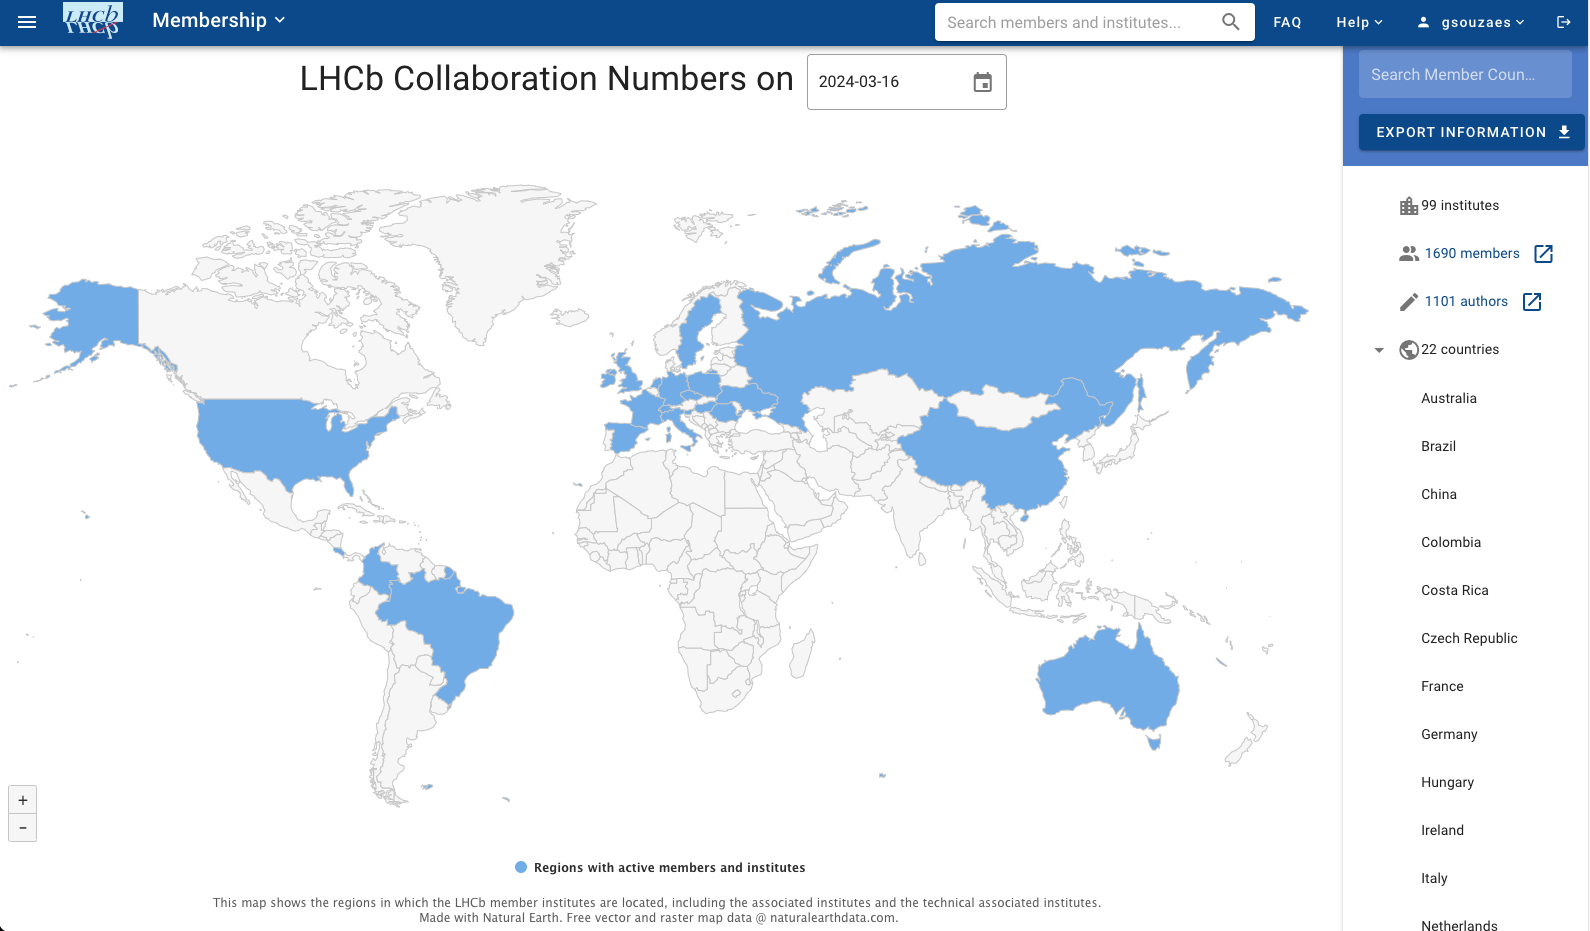
\includegraphics[width=1\linewidth]{figuras/collaboration_map.png}
    \caption{Countries that participate in the LHCb experiment.}
    \label{fig:collaboration_map}
\end{figure}


\begin{figure} [H]
    \centering
    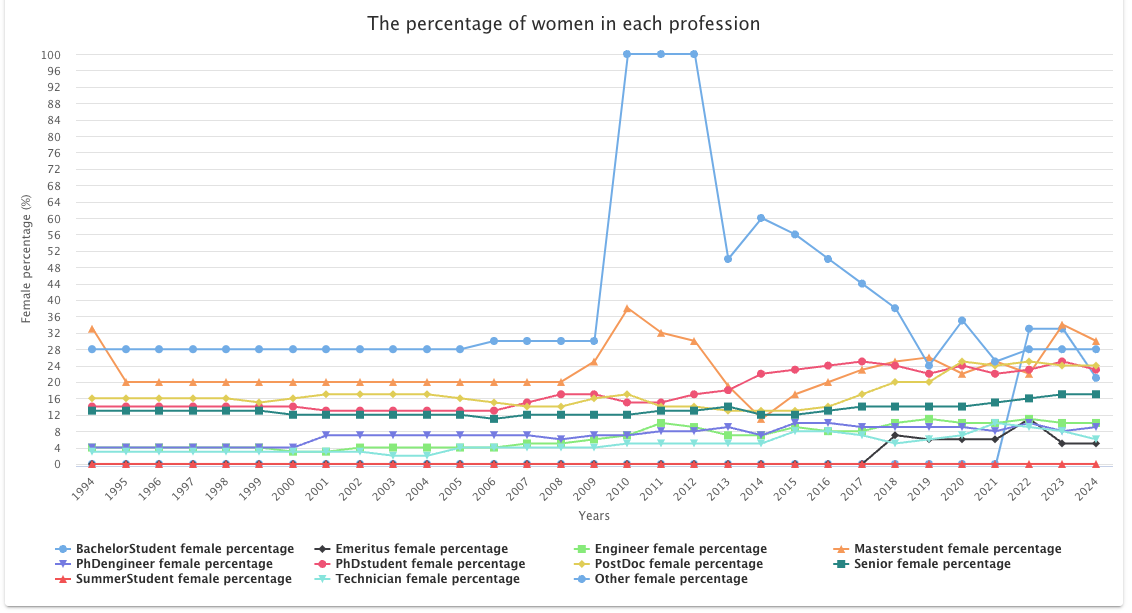
\includegraphics[width=1\linewidth]{figuras/gender.png}
    \caption{\textbf{Not real} (mocked) gender distribution data presented in the Membership.}
    \label{fig:gender}
\end{figure}

\paragraph{} Search interfaces for Appointments, Members, Institutes, and Employments facilitate data retrieval for the system's primary entities. Figure \ref{fig:homepage} illustrates the system's Homepage, which indexes all available views. From this central hub, users can navigate to specific search interfaces and access their Member and Institute profiles.

\begin{figure} [H]
    \centering
    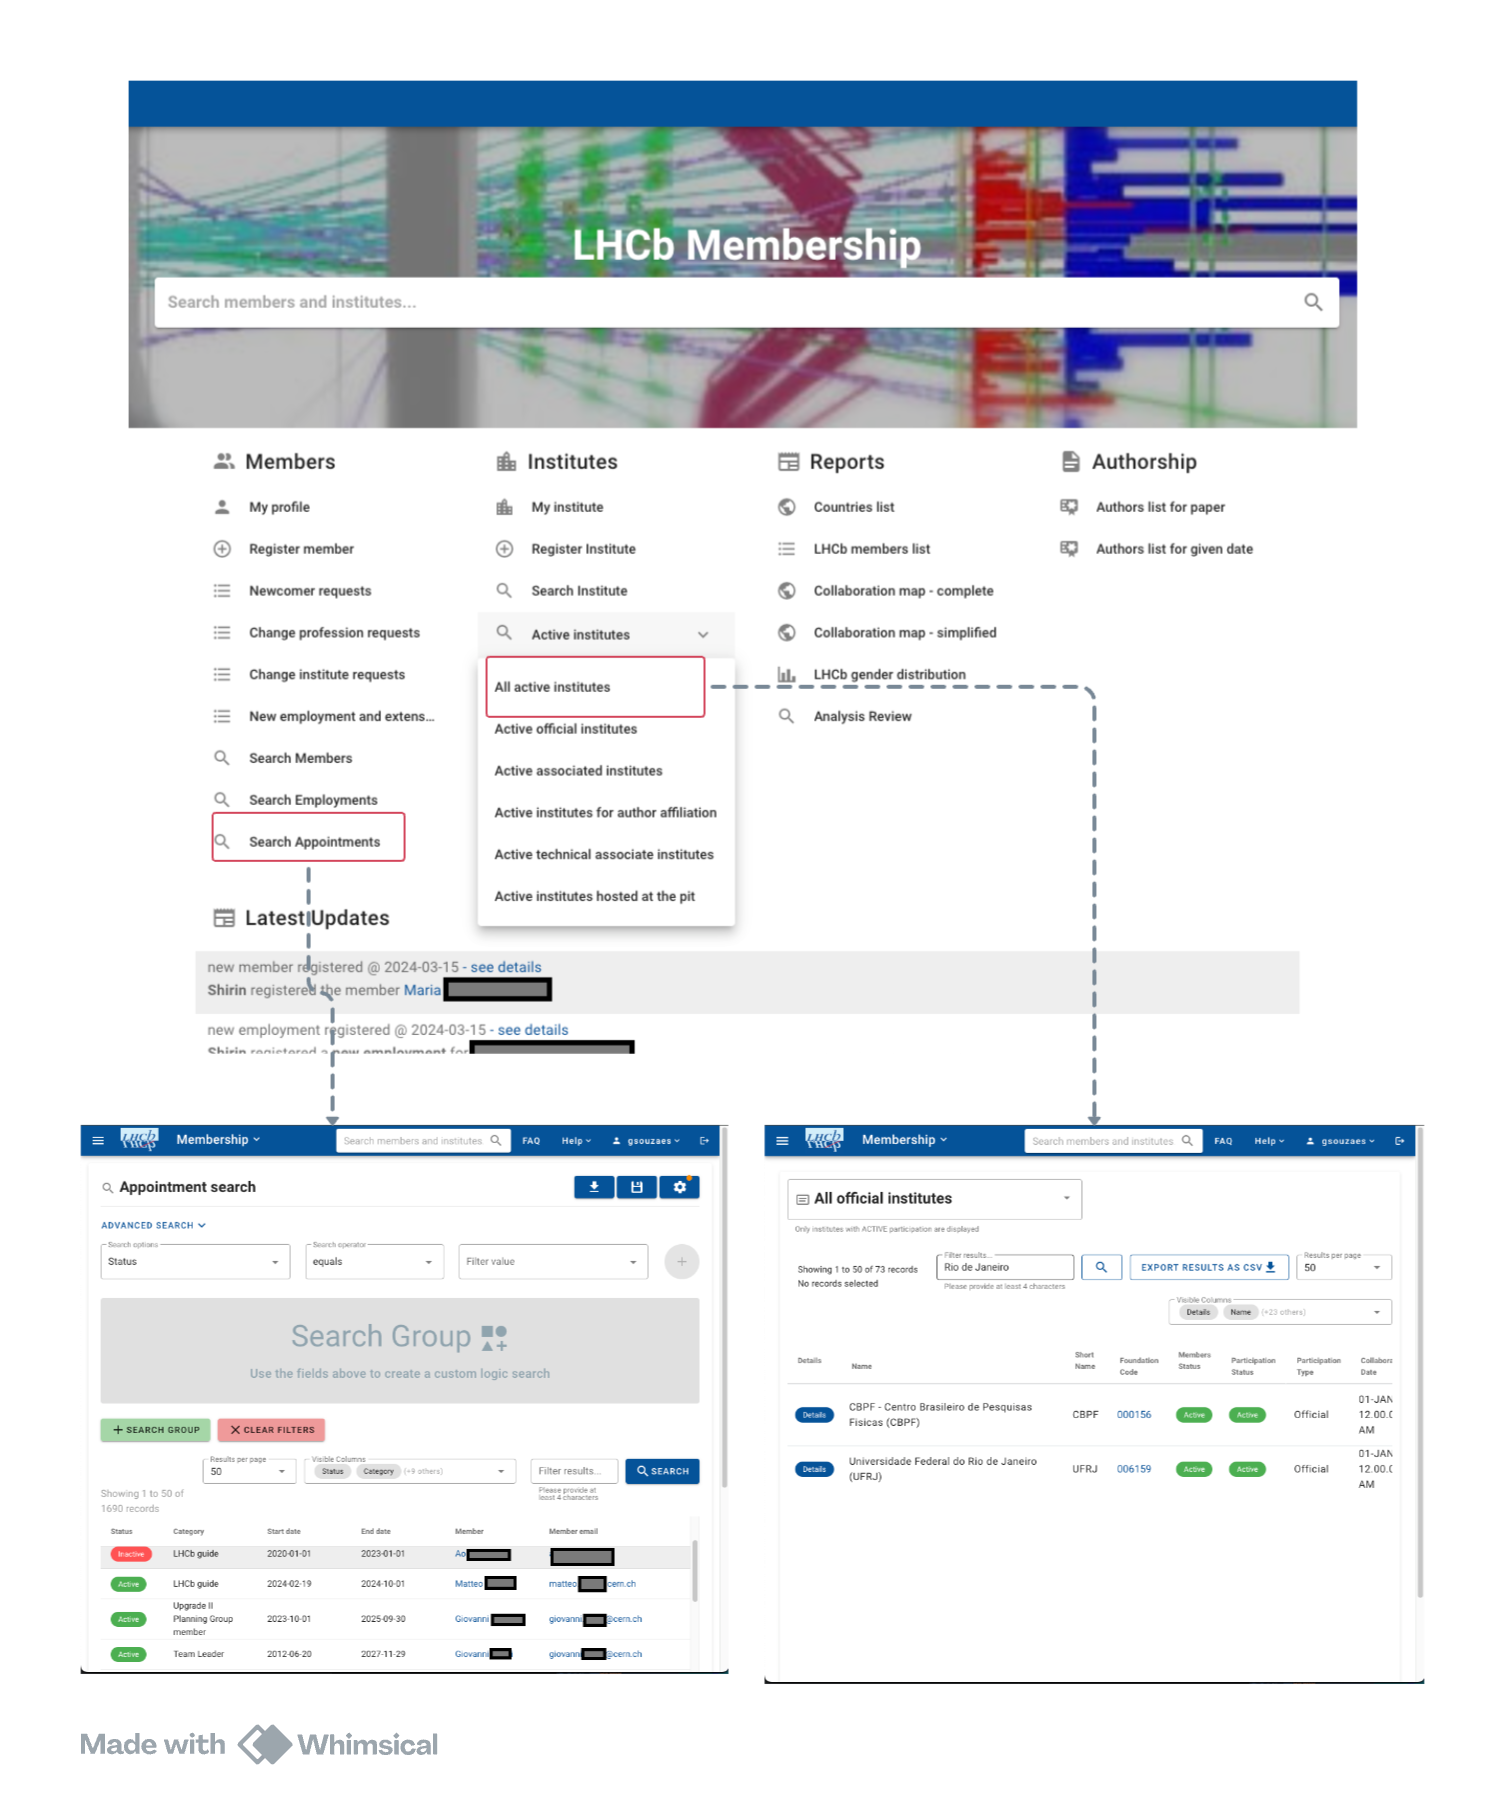
\includegraphics[width=1\linewidth]{figuras/homepage.png}
    \caption{LHCb Membership homepage and search interfaces.}
    \label{fig:homepage}
\end{figure}


\paragraph{} Data reports, including reminders for necessary actions, are dispatched via email through code in the Infrastructure Layer. This layer utilizes the same Application Layer Repository interfaces that the web Controller employs to display information in HTTP response bodies. A frequently dispatched email report highlights potential discrepancies between the Membership database and CERN's HR database, as depicted in Figure \ref{fig:email_report}. This inconsistencies report is sent to the Secretariat every Monday, enabling them to address and resolve them.

\begin{figure} [H]
    \centering
    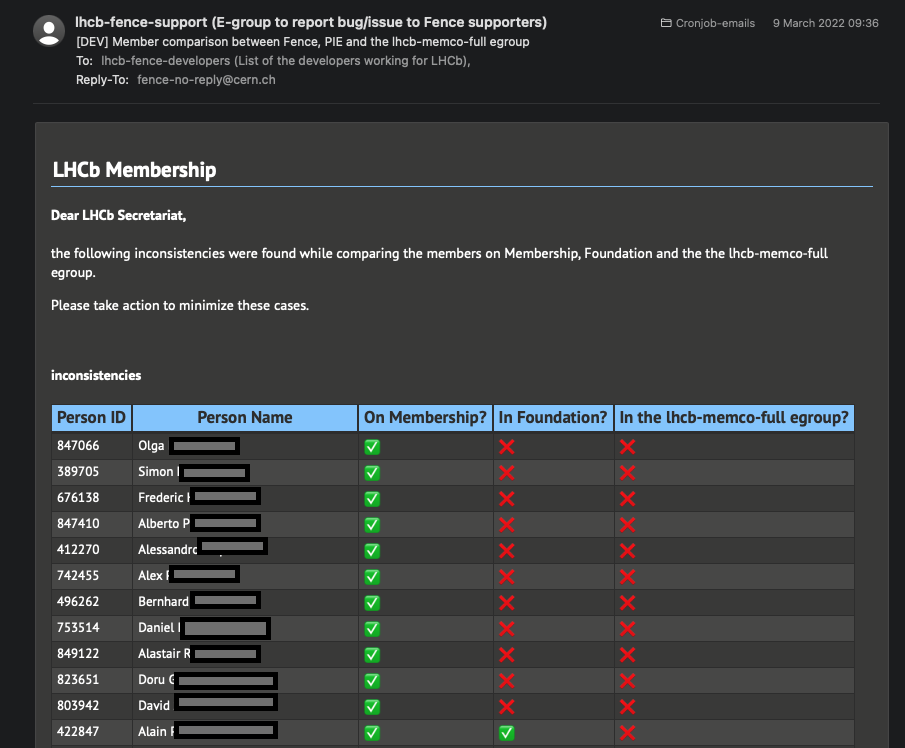
\includegraphics[width=0.8\linewidth]{figuras/email_report.png}
    \caption{Membership inconsistencies report sent weekly via email.}
    \label{fig:email_report}
\end{figure}

% ---------------------------------------------------------------
% Chapter 4 - Resultados
% ---------------------------------------------------------------
\chapter{Results}
\label{cap4}
\paragraph{} This chapter aims to identify evidence that the new architectural pattern has improved team productivity and enabled the system to offer functionalities that were not possible with the Fence version. To establish a timeline of events for correlation with the presented data: the Authorship system was deployed in March 2020; following its success, the LHCb Equipment Management System version 2 was released in September 2020; and the Membership Version 2 was released in May 2021.

\section{Cummulative flow chart}
\paragraph{}A Cumulative Flow Diagram (CFD) is a visual tool in Jira Software that tracks the status of project issues over time, providing a dynamic representation of workflow progress. It organizes work items into various statuses (done, blocked, to do, in progress, and in validation), plotted against time on the x-axis and the number of issues on the y-axis, with each area of the chart color-coded to represent different workflow statuses. This diagram is used for identifying workflow bottlenecks by revealing any segments that widen over time, indicating an accumulation of issues. An increase in ``Done" items, such as observed in Figure \ref{fig:cfc_jira} around the release date of the new Authorship and LBEMS systems, on a CFD generally signifies positive developments in project progress and team performance. This trend may indicate enhanced productivity as the team completes tasks more efficiently. It also suggests an effective workflow management strategy, timely meeting of deadlines, and successful issue resolution.

\begin{figure}[H]
    \centering
    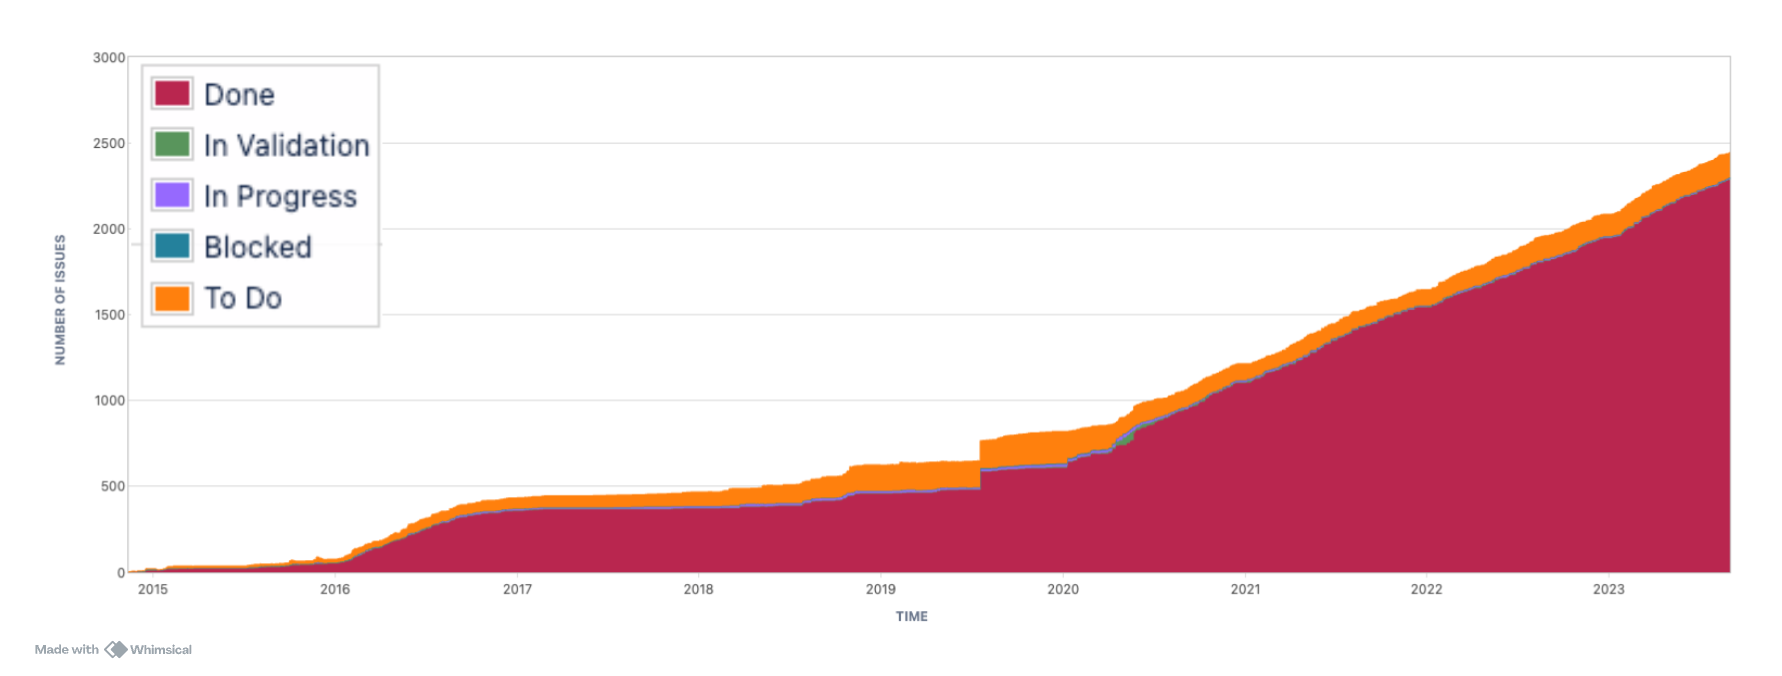
\includegraphics[width=1\linewidth]{figuras/cfd_subtitle.png}
    \caption{CFD graph extracted from Glance's Jira board.}
    \label{fig:cfc_jira}
\end{figure}

\section{Solved versus created report}
\paragraph{} The ``Solved vs.Created" report in Jira is a tool for tracking the rate at which issues are resolved compared to how many are created within a project over a specific period. This report shown in Figure \ref{fig:number_of_issues} plots two lines on a graph: one representing the number of issues created and the other the number of issues solved over time. An upward trend in the ``Solved" line relative to the ``Created" line in this report indicates positive project health and team efficiency. It suggests that the team is effectively addressing and resolving issues faster than new ones are being reported, contributing to the project's forward momentum. Consistently solving more issues than are created can lead to increased stakeholder confidence, as it demonstrates the team's capacity to handle challenges and maintain control over the project's scope. In Figure \ref{fig:number_of_issues} it is possible to notice an inflection point around the Authorship and LBEMS release dates, indicating performance gains by using the new architecture.

\begin{figure}[H]
    \centering
    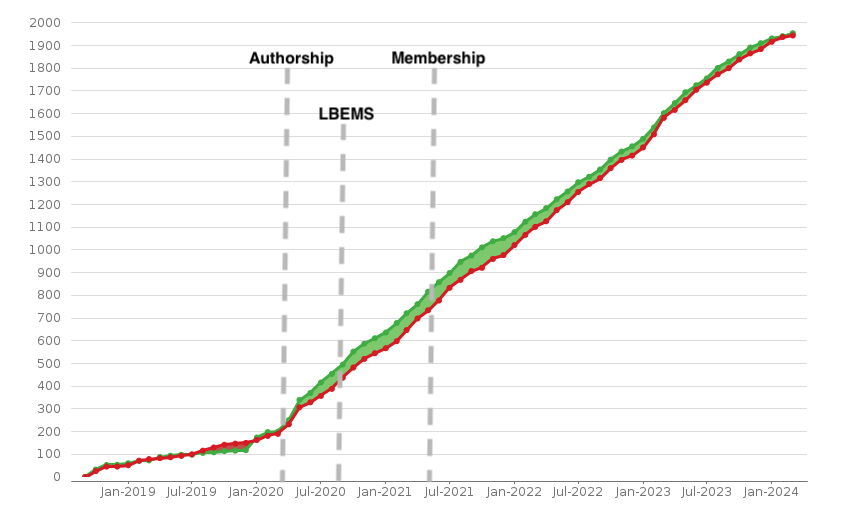
\includegraphics[width=0.7\linewidth]{figuras/number_of_issues_2.png}
    \caption{Solved vs. Created issues in the LHCb Glanace systems.}
    \label{fig:number_of_issues}
\end{figure}

\paragraph{} A pie chart displaying the distribution of issue types within a Jira Software project provides a visual breakdown of where the team's efforts are being allocated, categorizing issues into types such as stories, bugs, tasks, etc. An increase in the percentage of story issues and a decrease in the percentage of bug issues, as depicted in Figure \ref{fig:pie_jira}, can offer observations into the project's current phase and overall health. The shift towards a higher proportion of story issues as observed in Figure \ref{fig:pie_jira} might suggest that the project is in a phase of active development or feature expansion, with the team focusing more on adding new functionalities or enhancements. On the other hand, a decrease in the percentage of bug issues could signal improvements in the quality of the codebase or the effectiveness of the project's quality assurance processes.

\begin{figure} [H]
    \centering
    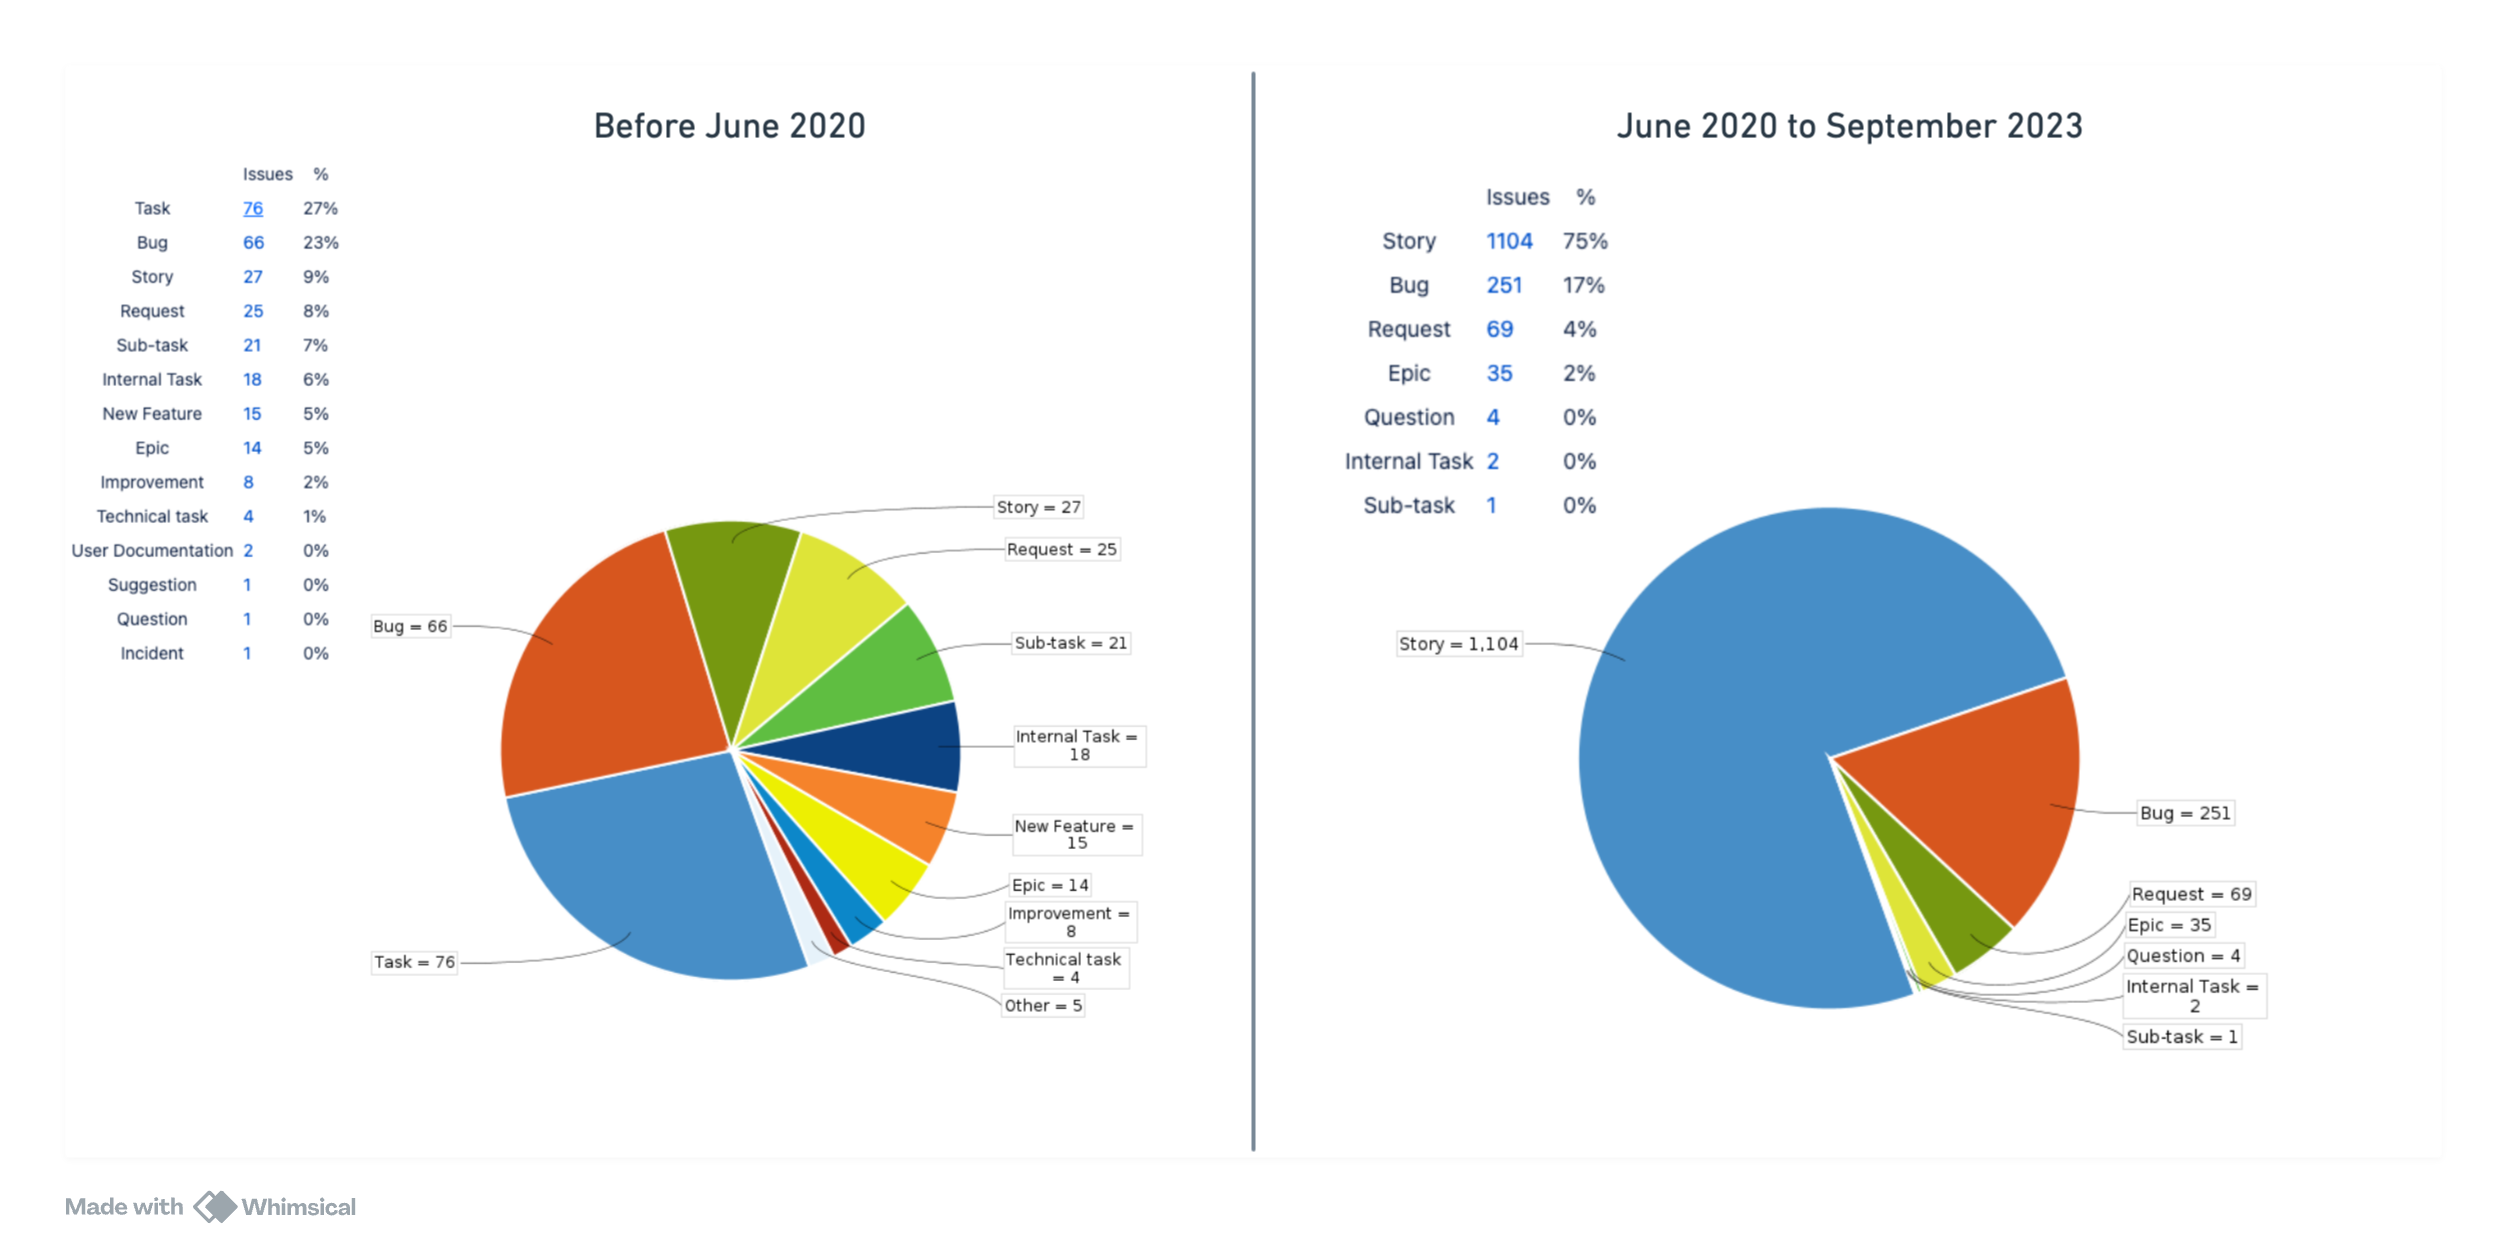
\includegraphics[width=1\linewidth]{figuras/pie_jira_2.png}
    \caption{Issues according to their type.}
    \label{fig:pie_jira}
\end{figure}






\section{Test coverage}
\paragraph{} In the version of the Membership system powered by Fence, automated testing was absent. With the introduction of a decoupled architecture in the subsequent iteration, automated integration testing was established to verify the stability of API endpoints against code alterations. Integration of these tests with Gitlab CI ensures that merge requests are only approved subsequent to the successful completion of all tests. This strategy, prioritizing integration tests, was influenced by the observation that modifications to the database and persistence layers were predominantly responsible for breaking changes. The distribution of test cases across different classes is illustrated in Table \ref{table:test_classes_and_numbers}.



\begin{longtable}{|p{0.5\textwidth}|p{0.4\textwidth}|}
\caption{Test Classes and Number of Tests}\label{table:test_classes_and_numbers}\\
\hline
\textbf{Test Class} & \textbf{Number of Tests} \\ \hline
\endfirsthead

\multicolumn{2}{c}%
{{\bfseries \tablename\ \thetable{} -- continued from previous page}} \\
\hline
\textbf{Test Class} & \textbf{Number of Tests} \\
\hline
\endhead

\hline
\endlastfoot

AppointmentTest.php & 12 \\
AuthorsListTest.php & 7 \\
CountryTest.php & 6 \\
EmploymentTest.php & 15 \\
GrantTest.php & 8 \\
InstituteTest.php & 11 \\
MemberTest.php & 14 \\
NewcomerTest.php & 10 \\
ParticipationTest.php & 4 \\
ReportTest.php & 3 \\
WorkflowTest.php & 27 \\
\end{longtable}



\section{Adoption by external systems}
\paragraph{} Two other web applications at CERN rely on Member information: the Speakers Bureau system, which assigns members to available talks and workshops, and the LHCb Shift system, which allocates members to shifts in the LHCb detector control room to assist in the 24/7 monitoring of the detector's operation. Prior to Membership Version 2, extracting data automatically from the Membership system was feasible only via direct database access, potentially violating OC11 regulations. Consequently, these systems would often maintain their internal lists of Members and Institutes, resorting to manual synchronization with the Membership database—the authoritative source for this data.

\paragraph{} The launch of Membership Version 2, which now offers a REST API, has significantly streamlined the process for related systems at CERN. These systems no longer require maintaining internal databases; instead, they directly access Member and Institute information via specific API endpoints. They can internalize this data through if needed and employ a polling mechanism to periodically refresh the information. To encourage and simplify integration, the Glance team developed a basic Python SDK (software development kit), recognizing that both applications are Python-based. This SDK abstracts the authentication and API call process, allowing for straightforward data retrieval through the \verb|search_member| method with the necessary search parameters. Listing \ref{lst:mb_sdk} showcases the \verb|search_member| function being used to find a specific member based on their CERN identifier. Listing \ref{lst:mb_sdk_implement} displays the \verb|search_member| method implementation, utilizing the \verb|get_api_access_token| function, also provided by the SDK, to retrieve the bearer token required for communicating with the Membership API.

\begin{lstlisting}[language=python, caption=Membership Python SDK usage., label=lst:mb_sdk]
from search_members import search_members

print(search_members(
    offset = 0,
    limit = 10,
    queryString = '"personId" =  "840720"'
    )
)

\end{lstlisting}

\begin{lstlisting}[language=python, caption=Membership SDK implementation., label=lst:mb_sdk_implement]
def search_members(offset, limit, queryString):
    load_dotenv()
    target_client_id = os.getenv('TARGET_CLIENT_ID')
    client_id = os.getenv('CLIENT_ID')
    client_secret = os.getenv('CLIENT_SECRET')
    api_base_url = os.getenv('API_BASE_URL')

    try:
        api_token = get_api_access_token(client_id, client_secret, target_client_id)
    except Exception as e:
        raise(Exception('Token exchange failed. Please check the user and the application credentials'))

    queryString = urllib.parse.quote_plus(queryString)
    url=f'{api_base_url}/members/search?offset={offset}&limit={limit}&queryString={queryString}'
    headers = {'Authorization': f'Bearer {api_token}'}
    #In case you need to use a proxy, uncomment both the following line and also the one on the request. You also need to set your proxy address and port
    #proxies = {"https": "http://127.0.0.1:54321"}

    try:
        response = requests.get(
            url,
            headers=headers,
            verify=False,
            #proxies=proxies
        )
    except Exception as e:
        print(e)
        raise(Exception('API call failed. Please check the API endpoint'))
    return response.json()
\end{lstlisting}




%\section{User experience survey}
%\subsubsection{Features}
%Whether or not the new version includes more useful features when compared to the old version

%\subsubsection{Look and Feel / Performance}
%How do you prefer the current look and feel when compared to the old one?

%\subsubsection{Stability}
%How often do you encounter unexpected behaviors when compared to the previous version? 

\section{Acknowledgements}

\paragraph{} A noteworthy and subjective outcome was the marked improvement in user satisfaction with the newly implemented systems. By employing Domain-Driven Design, developers were able to create features more closely aligned with real-life processes rather than generic, contextless CRUD operations. This enhancement in functionality received recognition in significant collaboration meetings, as illustrated in Figure \ref{fig:reconhecimentos}, underscoring the Glance team's growing significance at CERN and affirming the efficacy of the new architecture.

\begin{figure}[H]
    \centering
    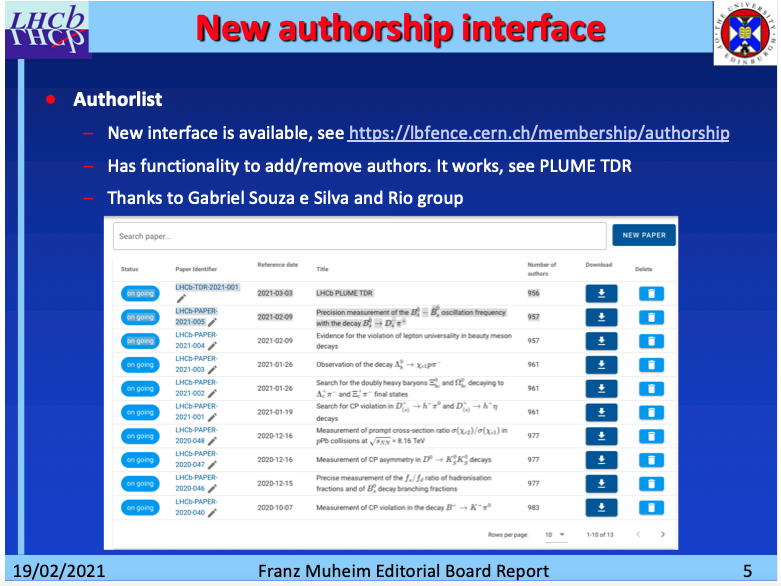
\includegraphics[width=1\linewidth]{figuras/reconhecimentos.png}
    \caption{Acknowledgement.}
    \label{fig:reconhecimentos}
\end{figure}





% ---------------------------------------------------------------
% Chapter 5 - Conclusão
% ---------------------------------------------------------------
\chapter{Conclusion}
\label{cap5}
\paragraph{} CERN provides a distinctive environment for teams to experiment, adapt, and advance technologies and processes. In this setting, the Glance team successfully overhauled the Membership system with a new architectural design. This initiative aimed to enhance system usability and incorporate previously unavailable features, stemming from the constraints of the Fence-based architecture. By re-evaluating Membership and Authorship requirements, it became evident that the system could be better tailored to support real-world processes. This realization underscored the need to transition to a technology sufficiently flexible to allow integrating the requested new functionalities. The development of the Authorship system, serving as a proof of concept for the Hexagonal Architecture with a decoupled backend API and frontend, allowed the team to standardize the Hexagonal Architectural pattern. This pattern not only established a standard approach for software development but also maintained the flexibility and modularity necessary for implementing complex and unique features such as the Search Library, implemented to fulfill the gap left by the Fence Super Search, unblocking the Membership refactor project. Following the establishment of the technology stack, Membership System Version 2 was launched by mid-2021. Subsequent to its release, two additional systems were developed using the same architectural principles, further validating the new architecture's robustness.

\paragraph{} Even though the new architecture facilitated the integration of novel features and yielded quantifiable productivity enhancements, areas for further improvement exist. The adoption of the Slim Framework 4 coupled with the application-specific middlewares in place of FRAPI could potentially boost performance. This transition would enable applications dependent on FRAPI, such as the Membership system, to perform configurations directly within the code rather than utilizing JSON configuration files, thereby avoiding file-read operations. This also gives developers the freedom to only install the middlewares that are actually going to be used by their applications. A great effort to remove FRAPI's CERN-specific middlewares to standalone bundles, particularly those managing authentication and authorization, is currently a priority for the Glance team allowing applications to combine these middlewares with the Slim Framework without FRAPI. Another aspect of possible enhancement on the backend is the implementation of more caching solutions. Given the frequent querying of numerous entities throughout the day, in-memory caching could significantly speed up common searches. CERN's proprietary server infrastructure offers developers a wide array of hosting options, further facilitating these improvements. On the frontend, transitioning the script section of Vue's SFCs from JavaScript to TypeScript would also be beneficial. TypeScript offers advantages over JavaScript, including static typing, class-based object-oriented programming, and compile-time error checking, which collectively enhance code reliability and maintainability. Another proposed enhancement involves refining the search interfaces to intuitively deduce the Search Field based on user input. For instance, if a user begins typing ``10/01...'', the system could automatically recommend date-related Search Fields, thereby streamlining the user interface from three inputs to a single, more intuitive input. This modification aligns with overarching principles advocating for simplified user interfaces. Lastly, upgrading from Vue 2 to Vue 3 would facilitate the adoption of the new Composition API, which provides a more flexible and modular approach to composing component logic. This upgrade would leverage the Composition API's advantages, including improved TypeScript support, enhanced reusability, and better code organization, thereby elevating the frontend development experience.



% ---------------------------------------------------------------
% Bibliografia
% ---------------------------------------------------------------
\normalsize
\cleardoublepage
\addcontentsline{toc}{chapter}{Bibliografia}
\bibliographystyle{coppe}
\bibliography{biblio}

% ---------------------------------------------------------------
% Apêndices 
% ---------------------------------------------------------------
   %\appendix
   % ---------------------------------------------------------------
   % Apêndice A
   % ---------------------------------------------------------------
   %\chapter{O que é um apêndice}
   %\label{ApendiceA}
   %\paragraph{}Elemento que consiste em um texto ou documento elaborado pelo autor, com o intuito de complementar sua argumentação, sem prejuízo do trabalho. São identificados por letras maiúsculas consecutivas e pelos respectivos títulos.
   % ---------------------------------------------------------------
   % Apêndice B
   % ---------------------------------------------------------------
   %\chapter{Encadernação do Projeto de Graduação}
   %\label{ApendiceB}
   %\begin{figure}
\begin{center}
\parbox[htb]{13.0cm}
  {
  \begin{center}
  
\includegraphics[scale=1.0]{Capa_do_Projeto_Final.eps}
  \caption[\small{Encadernação do projeto de graduação.}]{\label{FigPFC} \small{Encadernação do projeto de graduação.}}
  \end{center}
  }
\end{center}
\end{figure}
   % ---------------------------------------------------------------
   % Apêndice C
   % ---------------------------------------------------------------
\chapter{Stakeholder feedback}
\label{ApendiceC}
\paragraph{} Gloria Corti, a Senior Physicist at CERN, worked closely with the author to define the requirements for the Membership system and other systems used for radiological protection. Her feedback on the author's participation in the LHCb collaboration is attached below.

\begin{quote}
``Gabriel's work has been exceptionally good. He was very proactive and looked for solutions, taking into account constraints and possible outcomes and investigating all related aspects of a problem. He was always very conscientious and very careful to verify his work fulfilled the requirements given by the stakeholders. The work he did for the LHCb membership and the equipment management is highly valuable and eased administrative tasks of the LHCb secretariat and Radiation Protection Experts. We use the Glance systems almost daily. He put the basis of a modular, very powerful super-search and workflow management that we are exploiting in other new systems we are putting in place. He did it in a general way such that they can also be used by other experiments. In addition, he did so in the very difficult time of Covid, with the constraints it caused. Gabriel was also very good with transmitting his knowledge to the new students that joined him in LHCb and the other students working on Glance in the other experiments. For me, Gabriel was one of the best students we had, careful, thoughtful, and he became extremely competent in the two years he spent with us."
\end{quote}
   

\backmatter

\end{document}
